%% Documentation for RexxXML

%  The contents of this file are subject to the Mozilla Public License
%  Version 1.1 (the "License"); you may not use this file except in
%  compliance with the License. You may obtain a copy of the License at
%  http://www.mozilla.org/MPL/

%  Software distributed under the License is distributed on an "AS IS"
%  basis, WITHOUT WARRANTY OF ANY KIND, either express or implied. See the
%  License for the specific language governing rights and limitations
%  under the License.

%  The Original Code is RexxXML.

%  The Initial Developer of the Original Code is Patrick TJ McPhee.
%  Portions created by Patrick McPhee are Copyright � 2003
%  Patrick TJ McPhee. All Rights Reserved.

%  Contributors:

% $Header: C:/ptjm/rexx/rexxxml/RCS/rexxxml.tex 1.21 2003/10/31 16:10:46 ptjm Rel $


\documentclass[twoside]{report}

% twoside option adds extra margin for binding, but this does not
% work well for on-line viewing. It ought to be handled by the dvi
% or pdf processor.
\advance\oddsidemargin by \evensidemargin
\advance\oddsidemargin by -1in
\divide\oddsidemargin by 2
\evensidemargin=\oddsidemargin

% the pages are too short -- the goal here is not to have a lot of blank
% paper
\advance\textheight by 5\baselineskip
\advance\textwidth by 1in


% if run through pdftex, use ps fonts and turn on hyperlinking
\ifx\pdfoutput\undefined
 \def\rarrow{\ensuremath{\to}}
 \usepackage{hyperref}
\else
 \usepackage[pdftex,pdfborder=0 0 0]{hyperref}
 % uncomment for older hyperref (or update your hyperref!)
 % \def\pdfBorderAttrs{/Border [0 0 0]}%
 \def\_{\textunderscore\penalty\hyphenpenalty}
 \usepackage[T1]{fontenc}
 \usepackage{times}
 \usepackage{mathptm}

 \makeatletter
 \def\verbatim@font{\normalfont\ttfamily\small}
 \makeatother

 \font\symbol=psyr
 \def\rarrow{{\symbol\char174}}
 \pdfinfo { /Title (RexxXML Usage and Reference)
  /Author (Patrick TJ McPhee)
  /Subject (RexxXML User Guide)
  /Keywords (rexx,Regina,XML,XPath,XSLT)
  /Version (1.0.0)
  /Copyright (Copyright 2003, Patrick TJ McPhee)
 }
 \hypersetup{
  pdfstartview=FitH
  }
\fi

\lefthyphenmin=2
\righthyphenmin=3
\hyphenation{which-ever xml-Nodeset-Item at-tri-bute xml-Ver-sion xml-Add-Element
 xml-Node-set-Item xml-Node-Ptr}

\usepackage{array}
\usepackage{longtable}
\usepackage{makeidx}
\usepackage[pdftex]{graphicx}

% for function names -- normal font, put on parens, with a tick
% of space between them to keep them from flowing together
\def\fn#1{#1(\,)}

% for XML tags -- normal font, with left and right angle brackets
% (which have a steeper incline than greater/less-than)
\def\tag#1{$\langle$#1$\rangle$}

\makeindex

\newtoks\rcmsg

\begin{document}

\pagestyle{empty}

\null\vfill

\begin{center}

{\LARGE RexxXML Usage and Reference}

\vspace{18pt}

{\large Patrick TJ McPhee (ptjm@interlog.com)

\vspace{9pt}

Version 1.0.0

\vspace{9pt}

31 October 2003
}

\vfill


\includegraphics[width={6cm}]{tree}
\end{center}

\cleardoublepage

\pagenumbering{roman}
\pagestyle{headings}

\tableofcontents

\cleardoublepage

\pagenumbering{arabic}

\chapter{Introduction}

The RexxXML library provides a Rexx interface to data represented using HTML or
any XML dialect. The intent is to allow XML data to be processed in a
straight-forward manner within a Rexx program, and to allow Rexx to be
used from within certain XML-based applications.

Rexx is a programming language which was designed to be learned and used
easily by non-professional programmers. It is meant to make it easy to
write programs, at the expense of complicating the language
implementation. Its main characteristics are the absence of program
structure, isolation from machine limitations, integration with application
environments, and a set of built-in
functions which is useful for a wide array of data processing applications.

HTML is an SGML application which was designed for on-line
presentation of technical reports, and which is firmly entrenched as the
primary data representation on the world-wide web. XML is an SGML
application profile which was intended to allow greater freedom in marking
up web content, and which has gained some currency as a data exchange
protocol. It was specifically designed to simplify parsing (as compared
to the full generality of SGML) at the expense of complicating data
generation. Most document-generation-friendly features of SGML have been dropped,
even those which don't make parsing more complex.
In that sense, XML could be considered the anti-Rexx.
SGML\index{standards!ISO SGML} is an ISO standard language for defining document mark-up.

RexxXML's XML processing is provided by the Gnome project's libxml and
libxslt, both written by Daniel Veillard.
RexxXML does not attempt to provide a full interface to those
libraries, and it may provide less flexibility at the expense of greater
simplicity.  Books and other reference material about those packages can
still be helpful in using RexxXML.

This guide is both an introduction to XML processing using RexxXML and a
complete reference to the library. The reader is not expected to be familiar
with Rexx or XML syntax~-- I include a brief introduction to both, as
well as the XML-related technologies, XPath and XSLT~-- but additional
reference materials are needed to write effective programs.

\section{Installation}

The RexxXML package includes pre-compiled binaries for Win32
% and OS/2
platforms
and source code which should compile on those platforms and most Unix systems.
It does not include libxml, libxslt, or a Rexx interpreter.

The distribution also does not include an installation program. The
general installation instructions are to copy the appropriate library
file to an appropriate directory. From this package, only rexxxml.dll
(or, on Unix, librexxxml.so) is required to use the library,
and applications using it can be distributed with only this file.
The documentation file, rexxxml.pdf, should also be distributed if
end users are expected to write macros using these functions.

More specific instructions for each
platform follow.

\subsection{Win32}

If you don't have a Rexx interpreter, I suggest obtaining
\href{http://regina-rexx.sf.net}{Regina
Rexx}\footnote{http://regina-rexx.sf.net}.\index{getting!Rexx}\index{Rexx!getting} There are
several other interpreters available for win32 platforms. See
the\index{Rexx!Language Association}
\href{http://www.rexxla.org}{Rexx Language Association}\footnote{http://www.rexxla.org}
web site for details. Note that the port of Regina which was included
with the Windows NT resource kit is not suitable for use with libraries
such as RexxXML.

You must obtain libxml and libxslt from the
\href{http://xmlsoft.org}{libxml}\footnote{http://xmlsoft.org}\index{getting!libxml}\index{libxml!getting}
and
\href{http://xmlsoft.org/XSLT}{libxslt}\footnote{http://xmlsoft.org/XSLT}\index{getting!libxslt}\index{libxslt!getting}
web pages. My recommendation is to get the pre-compiled windows binaries
which are available from a link on those pages. RexxXML may or may not work with
binaries obtained from other sources. If you want to, for instance,
add Rexx support to an application which uses a non-standard build of
libxml, you may need to rebuild either RexxXML or the application.

There are two pre-compiled libraries in the distribution file. If you
use Regina, the appropriate file is RexxXML/win32/rexxxml.dll. If you
use any other interpreter, the appropriate file is
RexxXML/rexxtrans/rexxxml.dll, and you need to obtain RexxTrans from
\href{http://rexxtrans.sf.net}{its web site}\footnote{http://rexxtrans.sf.net}.

To install the pre-compiled library, copy the appropriate version
of rexxxml.dll to either a directory in your program search path or the directory
containing the Rexx executable.

See section \ref{sec:compiling} for information about compiling the
library from source code.

\subsection{OS/2}

I apologise that the OS/2 port has not been completed as of the initial
release of the library. I couldn't find libxslt at Hobbes, and the libxml
there is fairly old. I'll release it once I track down or build
OS/2 ports for these libraries.\index{to do!OS2/ port}

%The pre-compiled library RexxXML/os2/rexxxml.dll will work with either
%Classic or Object Rexx, probably on any 32-bit version of OS/2. It
%requires the EMX run-time environment, libxml, and libxslt, all of which
%are available from the \href{ftp://hobbes.nmsu.edu}{Hobbes FTP site}\footnote{ftp://hobbes.nmsu.edu}.

%Copy rexxxml.dll to a directory in your LIBPATH, and it should be ready
%to go.

\subsection{Unix}

The distribution does not include a configuration script, but it includes
make files which have been known to work using the stock vendor compiler
on several Unix systems. If you have one of those systems, link the
appropriate make file to the name `Makefile' and build the `dist'
target. For instance, on Solaris:
\begin{verbatim}
ln Makefile.sun Makefile
make dist
\end{verbatim}

On most platforms, this builds a shared library called librexxutil.so.
On HP-UX, the file is called librexxutil.sl, and on AIX, it's called
librexxutil.a. The path to this library can be set in three ways:

Most Unix systems allow a shared library search path to be embedded
into program files. If you build Regina (or your Rexx-enabled
application) such that this path is set to include a directory
such as /opt/regina/lib or /usr/local/lib, you can install
RexxXML by copying the shared library to this directory (see section
\ref{sec:compiling} for more information). If this is not possible,
you need to either set an environment variable or change the way
the system searches for shared libraries.

Unix systems typically use a different path for shared libraries than
they do for program files. The name of the environment variable used
for the shared library path is not standardised, however most systems
use LD\_LIBRARY\_PATH. Notable exceptions are AIX (LIBPATH) and
HP-UX (SHLIB\_PATH for 32-bit executables, LD\_LIBRARY\_PATH for
64-bit executables). To install RexxXML, add an appropriate directory
to the shared library path and copy the shared
library to that directory.

Finally, some systems provide a utility (often called ldconfig) which
can be used either to set the standard search path for shared libraries,
or to provide a database of shared libraries. On such a system, RexxXML
can be installed by copying the shared library to an appropriate
directory and using this utility to add it to the search database.
You'll need to consult your system documentation for more information.

\subsection{Notes on compiling}

\label{sec:compiling}\index{compiling}I provide make files for the
stock vendor compilers on several Unix systems. On Windows, I provide
make files for visual c++ (Makefile.nt) and the MinGW port of gcc
(Makefile.mingw).
%On OS/2, I provide a make file for the EMX port of gcc (Makefile.emx).
The Unix make files set platform-specific
variables and then load Makefile.inc, which contains the rules
for building the libraries. The win32
% and OS/2
make files contain all the
rules for building the library with their respective compilers.
I find it convenient to either link or copy the platform-specific
make file to the name Makefile.

The supplied make files expect libxml2 and libxslt to be installed
in the default location under /usr/local on Unix systems. You will
almost certainly have to edit the win32 make files to specify
the location of the include and library files.
Some parts of libxml and libxslt are optional (for instance,
schema support doesn't have to be compiled in). In this version
of RexxXML, compilation will fail if a required optional part of
libxml is not available. I will handle this better in a future
release. You may also have compile or link failures if you use
an older version of libxml or libxslt. The solution is to move
to the current versions of these libraries.

By default, the library is built with optimisation disabled and
debugging symbols included. This is convenient for library
development, however you'll get better performance
if you build the dist target (with the command `make dist').

To port the library to a new platform or to a new compiler on a
platform for which a make file exists, it should be sufficient to copy
an existing make file and change some of these variables. On Unix, to
change the compiler for an existing platform, it should be sufficient to
redefine PCFLAGS and POPT. If the new compiler is gcc, the values
can be taken from Makefile.bsd. The intent of each variable is indicated in
the table:

\goodbreak

\begin{longtable}{llp{9.5cm}}
\it Variable&\it Specific to&\it Purpose\\
\endhead
PDEBUG&Compiler&Flags in addition to -g required for creating programs
which can be examined in the debugger. This is relevant only if you
want to create a debug build;\\
POPT&Compiler&Flags which cause optimisation to be performed by the
compiler. At least -O should be used for all production code, in
my opinion;\\
PCFLAGS&Compiler&Compiler flags which should be set for both debug
and optimised compilation. This should include a flag for generating
relocatable (sometimes called position-independent) code;\\
PLDFLAGS&System&Flags for ld. This must include something
to cause ld to create a shared library, and a -L flag to give the
location of the libxml and libxslt libraries. On most platforms, it is
not necessary to link to the Rexx shared library, but you may
require special ld flags to ignore unresolved symbols;\\
PLIBS&System&Libraries required to resolve symbols used
in the library. This does not generally have to include the Rexx shared
library, since the Rexx interpreter will usually be running before
the library is loaded, but it must include -lxml and -lxslt, as
well as any libraries required by those libraries on your platform;\\
REXX\_INCLUDE&System&Compiler include flag to include rexxsaa.h
(defaults to --I/usr/local/include);\\
XML\_INCLUDE&System&Compiler include flag to include libxml/xmlVersion.h,
libxslt/xslt.h, {\it et al}
(defaults to -I/usr/local/include/libxml2);\\
XML\_LIBDIR&System&Flags to cause ld to find libxml2.a and libxslt.a
(defaults to -L/usr/local/lib).\\
\end{longtable}

The win32 make files have a different set of make variables. Due to the
nature of the win32 development environment, the distinction between
platform-specific and compiler-specific values doesn't exist.

\begin{longtable}{lp{12cm}}
\it Variable&\it Purpose\\
\endhead
DEBUG&Flags required for creating programs
which can be examined in the debugger. This is relevant only if you want
to create a debug build;\\
POPT&Flags which cause optimisation to be performed by the
compiler;\\
PCFLAGS&Compiler flags which should be set for both debug
and optimised compilation. This may include flags for creating relocatable code;\\
PLDFLAGS&Flags for linking. This must include something
to cause ld to create a DLL. The NT make files use the
compiler to link;\\
REXX\_INCLUDE&Compiler flag to set the directory containing rexxsaa.h;\\
REXX\_LIB&Full path to the Rexx library;\\
XML\_INCLUDE&Compiler flag to set the directory containing rexxsaa.h;\\
XML\_LIB&Either empty or a compiler flag to set the path to the
XML libraries;\\
PLIBS&Either a full path to the XML libraries or flags to include the
appropriate libraries, depending on the compiler.\\
\end{longtable}

\section{Reporting bugs}

I would like RexxXML to be useful and reliable. There will
always be room for improvement, and I appreciate hearing about problems.

If you do find a bug, an error in the documentation, or you simply have
a suggestion for improving the distribution, please send me details 
at ptjm@interlog.com. It's useful to know the operating system you're
using, the Rexx interpreter and its version, and the version of RexxXML,
and to have a set of steps for reproducing the bug. The example below
shows how to retrieve the interpreter and library version information:

\begin{verbatim}
/* report useful version information */
parse version ver
say 'Interpreter:' ver

call rxfuncadd 'xmlversion', 'rexxxml', 'xmlversion'
say 'RexxXML:' xmlversion()
\end{verbatim}

\section{Using RxFuncAdd}

RexxXML\label{sec:rxfuncadd} provides two entry points: xmlLoadFuncs\index{xmlLoadFuncs}
and xmlVersion\index{xmlVersion}.
xmlLoadFuncs must be loaded
using RxFuncAdd\index{RxFuncAdd}, and then invoked to register the rest
of the functions with the Rexx interpreter and initialise libxml and
libxslt.
RxFuncAdd takes three arguments~-- the name of the function as it will
be used in the Rexx program, the name of the library from which to load
the function, and the name of the function as it appears in the library.

RxFuncAdd returns 0 on success, or 1 on failure. Regina has a function
called RxFuncErrMsg\index{RxFuncErrMsg} which can give useful information about the reason
for a load failure. A few common reasons for failure are:

\index{RxFuncAdd!reasons for failure}Re-registration: RxFuncAdd will fail if
the Rexx function name (the first argument) duplicates a previously-registered
function. This sometimes happens with IBM's interpreter because functions
remain registered after a program finishes running, unless they are explicitly
dropped. You can test for this condition using RxFuncQuery;

Path issues: the library is called rexxxml.dll on Win32
% and OS/2
platforms,
librexxxml.a on AIX, librexxxml.sl on HP-UX, and librexxxml.so on
other Unix platforms. On Win32, this file needs to be in the path, or
in the directory containing the Rexx interpreter. On 
%OS/2 and 
AIX, it needs
to be in a directory listed in LIBPATH. On most other Unix systems, it
needs to be in a directory listed in LD\_LIBRARY\_PATH. Some systems
have an ldconfig utility which allows you to forego setting any environment
variables;

Case sensitivity: on some platforms, with some Rexx interpreters,
the case of the last two arguments to RxFuncAdd must match the
case of the library name as it appears in the filesystem and
the case of the function name as it appears in the library.
Try loading `xmlloadfuncs' rather than `xmlLoadFuncs',
and `rexxxml' rather than `RexxXML'. Regina allows you to omit the `lib'
prefix and any suffix. Other interpreters may require the full file name
to be included in the second argument;

Windows 95: early releases of windows 95 did not include msvcrt.dll, the
C run-time library used by RexxXML. This library is sometimes installed
with applications software. It can also be obtained through service packs,
or from the Microsoft web site;

%OS/2: the pre-built version of RexxXML requires the EMX run-time
%environment. This can be obtained from the Hobbes archive;

libxml, libxslt: you must have libxml and libxslt installed in the
appropriate locations. These are available through the
\href{http://xmlsoft.org}{libxml} web page;

Rexx.exe: Regina includes two executables, one called `rexx', and
the other called `regina'. The difference is that `rexx' includes the Rexx
interpreter as part of the executable, while `regina' loads the interpreter
from a shared library. RxFuncAdd works only with the `regina' version of
the interpreter (the `rexx' version is slightly faster, though). Other
interpreters typically have one executable called rexx.exe, which works
as you'd expect.

\section{Licensing}

RexxXML is distributed free of charge in the hopes that it will be
useful, but without any warranty. This version is distributed under the terms of the Mozilla
Public License. The precise details of the licence are found in the file
MPL-1.1.txt in the distribution.

If you use the library purely as distributed by me, then you can
cheerfully ignore the licensing. If you modify the source code or
adopt portions of it in your own programs or libraries, you should be
aware of and fulfil your obligations under the licence.

Although there are no obligations or restrictions related to use of the
library, I would prefer that you do not use RexxXML in applications
which cause injury or hardship to others. Also, if you derive a
significant monetary benefit from the use of RexxXML, please share a
portion with someone less fortunate. I'm always pleased to receive
good wishes, but Daniel Veillard and his contributers are responsible
for the bulk of the work.

\chapter{The Rexx Language}

Rexx was designed in the late 1970s by
\href{http://www.rexx.hursley.ibm.com}{Mike Cowlishaw}\footnote{http://www.rexx.hursley.ibm.com}
of IBM. His goal was to
create a language which would be simple enough for use by people who are not
professional programmers, and which can be integrated into operating systems and
application programs. This section gives an overview of the language which
should make it possible for readers unfamiliar with Rexx to understand the
examples later in the guide. There are several on-line introductions to the language (see the
\href{http://www.rexxla.org/Links/links.html}{Rexx Language Association}
web\index{Rexx!Language Association}
site for some links), and most interpreters include the reference information
needed to write actual programs. Cowlishaw's book {\it The Rexx Language} is
also a worth-while resource.

There are a few dialects of Rexx. Object Rexx is an object-oriented extension
which IBM introduced in the mid-1990s. Roo is a simpler object-oriented
extension by \href{http://www.kilowattsoftware.com/rooPage.htm}{Kilowatt
Software}\footnote{http://www.kilowattsoftware.com/rooPage.htm}. NetRexx is a java-based
dialect written by Mike Cowlishaw around the time Java was introduced. The
remaining dialects are loosely grouped together as `classic' Rexx, and differ
primarily in the built-in functions they provide. There is an ANSI standard\index{standards!ANSI Rexx}
for classic Rexx, and the general trend among implementations is to support
the functions and behaviour specified by ANSI. This section is an introduction
to classic Rexx.

\section{Overview}

A Rexx program consists of a sequence of statements, usually contained in a
single source file. There's no required formal structure~-- execution begins
with the first statement encountered, and continues until either there are no
more statements or the program exits explicitly. Variables do not have to be
declared, and do not have data types\index{data types!Rexx}~-- any variable can be used to hold any
kind of data. There are no reserved words, and variable names are not
case-sensitive.
Arithmetic is not limited by the machinery in use~-- calculations use
the precision specified by the programmer. These features reduce the work
needed to write simple programs.

At the same time Rexx has some features to help with writing longer
applications. The language supports sub-routines, which may be contained in
external files, and it has standard mechanisms for passing commands to a
controlling application and executing functions written in other languages. An
exception mechanism can trap the use of variables which have not been assigned
values, and there's support for rudimentary debugging built in to the
language.

Rexx is an interpreted language, which means the language instructions
are executed directly, rather than being translated into the instruction
set of the computer running the program. A program can generate a
statement and then call on the interpreter to execute it, which allows Rexx
programs to be self-modifying to some extent. Most language interpreters
convert the text representation of a program into a form which can be
easily and quickly executed. Rexx interpreters often allow this
intermediate form to be saved and restored, which can reduce the
start-up time for large programs, and which provides some protection
against program modification by end-users.

\section{Comments}

\index{comments!Rexx}Comments are parts of a program which can be used to provide
commentary directed at people reading the code. Often, comments will
explain what the program does and how
it does it, why a particular algorithm was used, or clarify obscure
code. They can also record information such as the name of the author,
current revision number, or copyright. 

In Rexx, comments begin with \verb+/*+ and end with \verb+*/+. Some
interpreters require that the first thing in every program be a comment,
and it's a good idea to at least record what the program does unless
you're planning to delete it as soon as it finishes running. There's
no limit on how long a comment can be, and they can occupy any number
of lines. The interpreter throws comments away as they are read, so
they have no effect on the program, except that a comment between
two symbols separates the symbols.

Comments nest, meaning each occurrence of \verb+/*+ within a comment
must have a corresponding \verb+*/+. The benefit of this is you can
easily comment out blocks of code. Apart from this, comments have no
syntactic requirements.

\begin{verbatim}
/* Program to demonstrate comments
   Patrick TJ McPhee, 2003/07/07 13.33.57 */

a = 3 /* a comment can go at the end of the line */
/* or at the beginning (but don't!) */ b = 4
c = a/* or in the middle */b
d = a/**/b * 2
e = (a/**/b) * 2

/* at this point, a = 3, b = 4, c = 34, d = 38, and e = 68
  /* this is a nested comment */
*/
\end{verbatim}

\section{Statements}

Anything that's not a comment is either an instruction to the Rexx
interpreter, a command to be executed by the controlling application, a
variable assignment, a label, a blank line, or a syntax error.
I'll distinguish between instructions, commands, and assignments,
and collectively refer to them as
`statements'.\index{statement}\index{instruction}\index{command}

Rexx instructions always begin with one of the keywords address, arg, call,
do, drop, else, end, exit, if, iterate, interpret, leave, nop, numeric,
options, parse, procedure, pull, push, queue, return, say, select, signal, then, or
trace, followed by other tokens, whose meanings depend on the keyword. Labels
consist of a symbol followed by a colon. Variable assignments consist of
a variable name, an equals sign, and an expression.
Any other non-blank lines must
consist of an expression whose value is passed to the controlling application.

\begin{verbatim}
'cp -p file1 file2'   /* string is evaluated and treated as a command */
a                     /* A is evaluated and treated as a command */
a = 3                 /* 3 is evaluated and assigned to A */
drop a                /* the drop instruction -- A is unassigned */
a:                    /* the label A */
\end{verbatim}

Statements are terminated by either a semi-colon or the end of the
line, whichever comes first, although they can be extended over more
than one line by placing a comma at the end of the line. This can lead
to confusion in some situations, so you should be careful to make such
a comma stand out.

Normally, instructions and assignments are written literally, while
a command is an expression which evaluates to
the command text. Occasionally, it's useful to create a Rexx instruction
dynamically, for instance, to allow a subroutine name to be supplied at
run-time. This can be done through the `interpret'
instruction\index{interpret}. The syntax is \verb_interpret_ {\it expression},
where {\it expression} evaluates to one or more valid Rexx statements. When using
literal strings in {\it expression}, one must be
careful to use enough quotation marks around strings that should appear in
the final statement.
\begin{figure}[htb]
\begin{verbatim}    
/* suppose fnname = 'myfn' and arg2 = 10. This statement is
 * equivalent to var = myfn("arg1, which is a string", 10) */
interpret 'var =' fnname'("arg1, which is a string",' arg2')'
\end{verbatim}
\removelastskip
\end{figure}

Note that to assign a value to a variable whose name is determined
dynamically,  you can
use the \fn{value} function, as discussed in section \ref{sec:assignment}.
This is likely to be more efficient and easier to read than `interpret'.

Rexx programs normally execute until they run out of statements, have
a fatal error, or encounter an `exit' instruction\index{exit}. The syntax is
\verb+exit+ {\it value}, where {\it value} is a numeric return code for the
program. Most operating systems expect this to be 0 for success or a non-zero
value for failure.

\section{Variables, constants, and expressions}

\subsection{Symbols}

Rexx expressions are
made up of symbols, literal strings, and operators.
A symbol\index{symbol!definition}\index{names!Rexx} is a combination of letters
(a--z)\index{letter!definition}, digits (0--9)\index{digit!definition},
question and exclamation marks (?!), underscores (\textunderscore) and periods
(.). Some other characters ({\it e.g.}, @, \$, and \#) can be used in
symbols with some interpreters. This is legal according to the standard,
but applications which take advantage of it will not be portable to other
interpreters\index{standards!gotta love them}.
Symbols are used for various purposes throughout Rexx programs.
Variable names, keywords, labels, and numbers are all types of symbol. 

When the Rexx interpreter encounters a symbol in a program, it first converts all
the letters to upper-case. This means two symbols which differ only in case,
for example \verb+if+ and \verb+If+, are treated precisely the same way
by the Rexx interpreter: Rexx symbols are case-insensitive.

\subsection{Variables}

Variables are mechanisms for storing values for later use. When we give
a variable a value, we say we are assigning a value to the variable, and
when we use the value, we say we are evaluating the variable, or that the
variable evaluates to some value.

In Rexx, a
variable's name can be any symbol, except for those that start with a digit or period.
Apart from that, there are no restrictions on the names which can be
used. It's legal to use a Rexx keyword (such as `options' or `signal') as a variable
name. There are certain variable names which you should avoid
using, though, since they are sometimes assigned values by the Rexx
interpreter: `rc', `result', and `sigl'.

Uninitialised variables\index{variable!uninitialised} evaluate to the variable's name, with all the
letters converted to upper-case (unless the novalue condition is in
effect~-- see section \ref{sec:conditions}). A variable can be assigned a value, then
returned to pristine condition using the `drop' instruction\index{drop}:
\begin{verbatim}
drop variable
\end{verbatim}

Variables with periods in their names are called compound
variables.\index{variable!compound}
The symbol up to and including the first dot is called the stem\index{stem}, and the
rest is called the tail\index{tail}. A value assigned to a stem acts as a default
for all compound variables based on that stem, and dropping the
stem causes all the compound variables based on that stem to be dropped.
We frequently refer to all the compound variables based on a single stem
as `a stem variable'.\index{variable!stem}

When a compound variable is evaluated, each
dot-delimited component of the tail is evaluated, then the tail is
appended to the stem, and the whole compound is evaluated. If \verb$i$
is equal to 3, \verb$x.i$ and \verb$x.3$ are the same variable.
The tails can contain any data. It can be numeric, a string, binary
data, or anything you like.

In many languages, a record\index{record structures} is a set of related
information, stored in the same variable. The data is accessible through a
fixed set of named components, called `fields'. Stems can simulate records by
using tails as fields. \verb$X.author$ could hold the name of a book's author,
for instance, while \verb$X.title$ holds its title. You need to be careful in
this case that you don't use `author' and `title' as variables, since that
would lead to bugs or at least make it less convenient to use the record
structure. One convention is to precede symbols which are being used as fields
with !, 0, or \textunderscore, and never start variable names with ! or
\textunderscore.

Arrays\index{arrays} are are also sets of information, however instead of having a
fixed set of fields, they form associations between one set of data,
the elements, and another, the indices. Array indices are commonly
restricted to be integers within some range (for instance, 1 to $n$,
where $n$ is the declared size of the array).
Rexx compound variables are like arrays which can can have any values for
indices. They can
simulate a numeric array by using the numeric index convention.
The numeric convention is for the 0 element to contain the number of array
elements $n$, while elements 1 to $n$ contain the data.\index{numeric
index convention}
A compound variable can simulate a multi-dimensional array by separating
the two dimensions with a dot.\index{arrays}

\begin{figure}[htbp]
\begin{verbatim}
/* print all the elements in an `array'. x.0 and each x.i.0 must
 * have been set when the array was assigned its values */
do i = 1 to x.0
  do j = 1 to x.i.0
     say x.i.j
     end
  end
\end{verbatim}
\removelastskip
\end{figure}

One significant difference between stems and arrays or records in other
languages is that a stem is not a single variable. You cannot assign one
stem to another or pass it to a function, although you can pass the name of a stem
to a function.
\index{variable!compound}\index{variable!stem}

\subsection{Assignment}

\label{sec:assignment}Variables can be set using an assignment statement, the `value' function,
the `parse' instruction, loop iteration, and by functions such as the
ones in the RexxXML package. Here are a few examples:

\begin{verbatim}
var = value /* evaluates `value' and assigns the result to var */
call value 'var', value /* does the same thing -- here, value is
                           both a function name and a variable
                           used as a function argument */ 
parse var value var     /* does the same thing -- here, var is
                           both a keyword and the name of a
                           variable used in a template */
\end{verbatim}

An assignment statement is a variable name, an equals sign (=), and an
expression (see sections \ref{sec:arithmetic}, \ref{sec:strings}, and \ref{sec:conditionals}).
It evaluates the expression and assigns the result to the variable.

The parse\index{parse}\label{sec:parse} instruction is probably the most complicated thing in Rexx and
a full treatment goes well beyond my goals for this overview.
The most general syntax is \verb+parse+ {\it something} {\it template}.
It
evaluates {\it something}, then breaks the result into fields and assigns them
to variables according to {\it template}. Examples in this guide will
use \verb+parse var+ {\it variable} {\it template}, which evaluates a variable,
\verb+parse value+ {\it expression} \verb+with+ {\it template}, which evaluates an arbitrary
expression, and \verb+parse arg+ {\it template} \verb+,+ {\it template} \dots, which
evaluates an argument list. In this case, {\it template} is repeated for each
expected argument of a subroutine.

Parse templates can be confusing, however in this guide only two simple
types are used: the list of variables, and the list of variables
separated by literal strings. When the template is a list of variables,
the value being parsed is broken up at spaces, and each field is assigned
to the corresponding variable from the list.
When variable names are separated by a literal string, the string value is
used as a delimiter instead.
Periods (.) can be used instead of variable names in any parse template,
in which case the corresponding field is discarded rather than being
assigned to a variable.
If there are left-over variables after all the fields have been assigned,
they are assigned the zero-length string. If there are not enough variables
to hold all the fields, the last variable is assigned all the left-over fields and
delimiters. It's common to use this feature to extract fields from a variable, one
field at a time.

\begin{verbatim}
parse value 'go to the store' with g t th s
/* g = 'go'; t = 'to'; th = 'the'; s = 'store' */

parse value 'alpha,bravo,charlie,delta' with a ',' b ',' . ',' d
/* a = 'alpha'; b = 'bravo'; d = 'delta' */

list = 'one two three'
parse var list car list
/* car = 'one'; list = 'two three' */
\end{verbatim}

The \fn{value} function either retrieves or sets the value of a specified
variable. Its first argument is an expression which evaluates
to the variable name, while the second is the value to assign to the
variable. The variable can be a Rexx variable or a variable in some
controlling environment, in which case the optional third argument defines
the environment in which
the variable is found. As I mentioned earlier, the \fn{value} function can be
used instead of the interpret instruction in cases where the variable
name to be updated is itself generated dynamically. I'll mention later
that \fn{value} can be used in a subroutine to access the contents of
a stem variable whose name has been passed as an argument.

\begin{verbatim}
call value var,val        /* set value of a variable whose name
                             is stored in the variable `var' */
val = value(arg(2)'.'i)   /* val = x.i, where x is the second
                             argument */
\end{verbatim}

Loop iteration and the RexxXML functions are discussed later.

\subsection{Constants}

Data in Rexx is treated as strings of characters. The strings can be read
from an external file or queue, returned by a function, or generated from constant
values stored in the Rexx program.
There are three kinds of constants: numeric symbols, strings, and
non-numeric symbols. 

Numeric symbols\index{number!definition} are simply real numbers as they are usually expressed in
English-speaking countries. They consist of digits with an optional
sign and an optional
period representing the decimal, followed by an optional exponent. The
exponent is e or E followed by an optional sign followed by digits, and
it means to multiply the rest of the number by 10 raised to the power
of the number to the right of the E.

Constant strings\index{string!definition} are sequences of characters delimited by either
\verb+'+ or \verb+"+. The string delimiter can be represented by
doubling (\verb+'it''s'+) or by using the other delimiter
(\verb+"it's"+). A string may be represented in hexadecimal by
appending `x' to it, or in base-2 by appending `b' to it.

\begin{verbatim}
x = .232             /* assign a number to x */
x = '.232'           /* exactly the same */
x = '2e 32 33 32'x   /* exactly the same, hexadecimal */
x = '2e323332'x      /* exactly the same */
x = '00101110001100100011001100110010'b /* but why? */
\end{verbatim}

A symbol\index{symbol!constant} which is not a number ({\it e.g.}, it contains a letter other
than e) but which is not a valid variable (starts with period or a digit)
is a constant whose value is itself upper-cased. This can be useful for
creating field names in a record represented by a compound variable\index{record structures}, however you should
know that ANSI\index{standards!ANSI Rexx} Rexx has reserved all symbols starting with period for
future `special' variable names.

\subsection{Arithmetic}

\label{sec:arithmetic}
Rexx provides arbitrary-precision arithmetic\index{arithmetic!arbitrary precision}. What this means is that
you can perform calculations to however many digits of accuracy you want,
within the limits of sanity, keeping in mind that some interpreters may have a
restrictive
definition of sanity. The default precision is 9, which is often too low.
Keeping in mind the time cost of calculations increases with the number
of digits of accuracy, I suggest\index{arithmetic!precision}\index{numeric digits}
using 20 digits for most purposes:
\begin{verbatim}
numeric digits 20
\end{verbatim}

Precedence\index{precedence!definition} is a weighting assigned to operators which determines which
operation is performed first when two operators appear in a row. Rexx
evaluates expressions in order of precedence, and the left to right.

The standard arithmetic operations are supported with the precedence set so
that they work the way you
might expect. Parentheses can be used to ensure the correct grouping of
operations. $3+2*5$ is 13, but $(3+2)*5$ is 25. The operators and their
precedences are:\index{arithmetic!precedence of operators}\index{precedence!arithmetic operators}

\begin{longtable}{llp{7.7cm}}
\it Operator&\it Precedence&\it Effect\\
\endhead
$+$&8&(as prefix) multiplies the next term by $1$\\
$-$&8&(as prefix) multiplies the next term by $-1$\\
$**$&7&raises the term to the left to the power of the integer term to the
right\\
$*$&6&multiplies the term to the left by the term to the right\\
$/$&6&divides the term to the left by the term to the right\\
$\%$&6&divides the term to the left by the term to the right and strips off
the non-integer portion\\
$//$&6&divides the term to the left by the term to the right and returns
the integer remainder\\
$+$&5&adds the term to the left to the term to the right\\
$-$&5&subtracts the term to the right from the term to the left\\
\end{longtable}


Cowlishaw's book contains a complete description of how calculations
are performed. I will say that the highest precedence\index{arithmetic!precedence of operators}\index{precedence!arithmetic operators}
operators are applied first, and equal precedence operations are applied left-to-right.
Note that $-x\mathbin{**}2$ is equivalent to $(-x)\mathbin{**}2$ or $x^2$, and not $-x^2$ as
you might expect.

Rexx does not include very many arithmetic functions, and in particular there
are no transcendental functions\index{arithmetic!transcendental functions}.
Some interpreters include these functions
as a loadable library, however they generally do not provide arbitrary
precision. There are also math libraries written in Rexx available on
the Internet, although there is currently no Rexx archive, so finding them
can be a challenge. I provide
a `mathematical bumper pack' from
\href{http://www.interlog.com/~ptjm}{my web
page}\footnote{http://www.interlog.com/\textasciitilde ptjm}. This
includes two math libraries written in C and an old version of
John Brock's RxxMath library, which is written
in Rexx and provides arbitrary precision.

The standard language does provide functions for converting between bases 2,
10, and 16 (\fn{b2x}, \fn{d2x}, \fn{x2b}, \fn{x2d}), for creating characters from
their character codes, expressed in bases 10 and 16 (\fn{c2d}, \fn{c2x},
\fn{d2c}, \fn{x2c}), for determining absolute value (\fn{abs}, maxima and minima
(\fn{max}, \fn{min}), decimal place conversion (\fn{format}, \fn{trunc}), and the
sign of a number (\fn{sign}), as well as a pseudo-random number generator
(\fn{random}).

\subsection{String manipulation}

\label{sec:strings}
Rexx has three ways to concatenate strings:\index{string!concatenating}
placing two expressions next to each other, separated by a space,
concatenates their values, with a space between them.
Placing two expressions next to each other, without so much as a space
between them, concatenates their values without a space between them.
This is only possible for certain kinds of expressions,
for instance a string followed by a variable other than `x' or `b'.
Finally, there's
the concatenation operator $\|$, which has the same effect as abutment, but
doesn't require the strings to be abutted.
Technically, you can abut any two expressions by placing a comment between them,
but it's simpler and clearer to use the concatenation operator.
Compared to the operators in the tables in sections \ref{sec:arithmetic}
and \ref{sec:conditionals}, the concatenation operators have precedence
4.\index{precedence!string operators}

\begin{verbatim}
x = 'nice'
y = 'day'
z1 = x || y    /* z1 = 'niceday' */
z2 = x y       /* z2 = 'nice day' */
z3 = x/**/y    /* z3 = 'niceday' */
z4 = x''y      /* z4 = 'niceday' */
\end{verbatim}

You can parse data from strings using the `parse' instruction\index{parse} (section
\ref{sec:parse}) and compare strings as described in section
\ref{sec:conditionals}, but all other string operations are performed
using built-in or third party functions. Hopefully the use of functions
in the examples will be self-explanatory, but here are a few examples of
functions I'm likely to use:

\begin{verbatim}
z1 = strip(' exceptional ')      /* z1 = 'exceptional' */
z2 = substr('demanding', 3, 2)   /* z2 = 'ma' */
z3 = substr('demanding', 3)      /* z3 = 'manding' */
z4 = insert('r', 'mable', 2)     /* z4 = 'marble' */
z5 = changestr('a', 'wat', 'i')  /* z5 = 'wit' */
z6 = word('go by brooks', 2)     /* z6 = 'by' */
z7 = words('what passing bells') /* z7 = 3 */
z8 = wordpos('b', 'a b c')       /* z8 = 2 */
z9 = abbrev('water', 'wat')      /* z9 = 1 */
z10 = abbrev('water', 'wit')     /* z10 = 0 */
z11 = compare('water', 'wat')    /* z11 = 4 */
z12 = compare('water', 'water')  /* z12 = 0 */
z13 = pos('t', 'water')          /* z13 = 3 */
z14 = translate('water')         /* z14 = 'WATER' */
z15 = translate('horse', 'wrtae', 'heros') /* z15 = 'water' */
z16 = translate('horse', 'ndrik', 'shore') /* z16 = 'drink' */
\end{verbatim}

A table of the built-in functions in the ANSI standard appears in section
\ref{sec:builtins}.

\section{Subroutines}

\label{sec:subroutines}
A subroutine is a named collection of code which can be executed repeatedly.
It may return a value, in which case it's called a function, or it may simply
do something useful~-- this is known as having side-effects. Similarly, some
subroutines can act on any data in the program, while others act only on data
which is explicitly passed to them. The latter type of subroutine is called a
procedure\index{procedure!definition}. The data passed to a subroutine is
called its arguments.

Rexx subroutines can be defined in the Rexx program, loaded from external Rexx
files, executed as stand-alone executable programs written in any language,
called procedures written in another language and interfaced through a
standard programming API, or they can be built in to the Rexx interpreter.

\subsection{Calling subroutines}

In any case, the subroutine is executed either using the `call' instruction\index{call} or
a function call expression. The operands of the call instruction are the
subroutine name, which is either a symbol or a literal string, and a
comma-separated list of its arguments\index{arguments!call instruction},
each of which can be any expression. Note that subroutine arguments should
not have parentheses around them when used with the call instruction, although
older versions of the Regina interpreter allow this. If
a function is executed using the `call' instruction, its return code is written to the variable
`result'.

A function call expression consists of the subroutine name, an
open parenthesis, a comma-separated list of the arguments, and a close
parenthesis\index{arguments!function call}. The value of the
expression is the return code of the function. You should always use this value for something~-- if you
simply make a function call without at least assigning the return code to a
variable, the return code will end up being passed to the controlling
environment, which is likely not what you want. See section
\ref{sec:environments} for further discussion. If a subroutine which
doesn't return a value is used in a function call expression, an error
condition is raised.

In both the call instruction and the function call expression, you can put quotes
around the subroutine name, making it a literal
string.\index{string!subroutine name}
Putting quotes around the function name has two effects: it prevents the
interpreter from executing a locally-defined subroutine, and it
prevents the interpreter from converting the name to uppercase. This may
be necessary to execute an external command on a system such as Unix,
where the file system is case-sensitive. It can also be used to replace a
built-in function with a user-written one. The built-in can be called
from its replacement by including the name in quotes.

\begin{verbatim}
/* normal function calls */
call fn arg1, arg2, arg3
rcc = fn(arg1, arg2, arg3)

/* the return code of fn() will be passed to the controlling
 * environment */
fn(arg1, arg2, arg3)

/* accepted by older versions of Regina, but invalid syntax */
call fn(arg1, arg2, arg3)

/* quotes may be needed to call an external routine */
files = 'ls'('*.c')
\end{verbatim}

\subsection{Defining internal subroutines}

A subroutine is defined by placing whatever instructions are necessary between
a label\index{label!internal subroutine} and a return instruction. A
label\index{label!definition} is a symbol followed by a colon. A return
instruction\index{return} is `return' followed by an optional value.

To make the subroutine a procedure, follow the label with
`procedure'.\index{procedure} It's a good idea to do this, since you can
otherwise end up with a variable name conflict. If you unintentionally use the
same variable name in your main program and in a subroutine called by the main
program, the subroutine may unexpectedly change the main program's variable.
Since variables with the same name likely hold similar kinds of data, bugs of
this nature might not be obvious, so it's best to use `procedure' with all
your subroutines rather than waiting to be bitten by a conflict.

It's best to pass all the values needed by a subroutine as arguments,
but if that's inconvenient or if you need to change a variable in the caller,
you can
make some variables available using the `expose' keyword. The syntax is
\verb+procedure expose+ followed by a list of variable names to expose.
If you give a stem in the list, all compound variables based on that stem
are exposed. If you put a variable name in parentheses, the variable is
evaluated and the result is the name of the variable to expose.

The procedure instruction effectively builds a wall between the
subroutine and its caller. The expose keyword adds a door to the wall,
but gives only certain variables the key. This wall is in place until
the subroutine returns, and it affects variable evaluation not only
for the subroutine which built it, but for any subroutines which are
called while the wall is in place. Variables used in a nested
subroutine call can be exposed only as far as its callers allow.

In the figure, sub1 is a procedure which exposes variables x and z, sub3 is a
procedure which exposes x and y, and sub2 is not a procedure at all. If the
main program calls sub1, sub1 calls sub2, and sub2 calls sub3, a reference to
\verb$x$ in any of the subroutines affects the variable in the main program, a
reference to \verb$y$ affects to the variable in sub1, and a reference to
\verb$z$ affects the variable in sub1 if the reference occurs in sub1 or sub2,
but to the local variable if it occurs in sub3.

\includegraphics{procedure}\index{hoping to avoid confusion!seriously}

\label{sec:arguments}Subroutine arguments are accessible using the `parse
arg'\index{parse!arg}\index{arguments!accessing} instruction,
or the \fn{arg} function. The `arg' instruction\index{arg}
works like `parse arg', but also converts the data to upper-case.
The syntax of `parse arg' is \verb+parse arg+ {\it template} \verb+,+
{\it template} \dots, with a comma-separated parse template for each
expected argument. Parse templates are discussed briefly in section
\ref{sec:parse}. Normally, in an argument list, each parse template
consists of a single variable, so that each argument is assigned to
a variable. Full parse templates are allowed, though, so you,
on the one hand, can go to town parsing arguments if that's helpful,
but on the other hand need to be careful not to omit the commas in the
parse instruction.

\begin{verbatim}
/* add up the elements of a stem and return the number of
 * elements. The sum is returned in the global variable w */
countandsum: procedure expose globals., w
  do i = 1 to globals.0
     w = w + globals.i
     end
  return globals.0

/* concatenate two strings, with the longest first */
lcat: procedure
  parse arg first, second
  if length(first) > length(second) then return first || second
  else return second || first

/* add together n variables */
sum: procedure
  s = 0
  do i = 1 to args()
    s = s + arg(i)
    end
  return s
\end{verbatim}

One important limitation of the language is that it's not possible
to pass a stem to a subroutine as a unit. It is possible to
pass the name of a stem. Compound variables based on the stem can then be
accessed using the \fn{value} function. Associative arrays which work much like
stems but can be passed to subroutines are provided by the
RxHash\index{RxHash} package, which is available from \href{http://www.interlog.com/~ptjm}{my web
page}.

When you have subroutines defined at the bottom of your main program,
you should exit the program before the subroutine definitions, using the
exit instruction. If you fail to do this, you will either confuse
yourself wondering why extra stuff is happening after the program has
finished, or you will get an error at the first `procedure' instruction.

\begin{verbatim}
/* rcc is the integer return code, usually 0 for success */
exit rcc
/* subroutine definitions follow */
\end{verbatim}

\subsection{Defining external subroutines}

An external subroutine is simply a file with a Rexx program
which ends in a return statement. Such subroutines are always procedures -- they
cannot access any variables except for the ones passed as arguments.

The name of the subroutine is the name of the file which contains it.
Since file names can
be incompatible with the syntax for symbols ({\it e.g.}, file names
often include lower-case letters, while symbols are always
all-uppercase), the function name can and sometimes must be enclosed in quotes when
calling external functions.\index{string!subroutine name}

Different interpreters have different search path conventions, but
there's always some way to specify a directory where external subroutine
files can be stored. Consult the interpreter's documentation for details.

\subsection{Using programs as subroutines}

Some interpreters allow any program to be invoked as a function, usually
with the standard output of the program as the return value. This is not
implemented portably, though. For instance
\begin{verbatim}
x = 'ls'()
\end{verbatim}
is accepted by both Regina and Rexx/IMC, but the value of x is not the
same, since Regina converts new-lines to spaces, while Rexx/IMC
does not.

For systems like Unix which have case-sensitive file systems, you need to
put quotes around the program's name, unless it's all upper-case
itself.\index{string!subroutine name}

\subsection{C function libraries}

Most Rexx interpreters can call specially-defined functions, usually
written in the C language. This allows specialised or computationally
intensive functionality, such
as parsing XML files, to be written in an efficient language, while program
logic is written in Rexx. RexxXML is an example of such
a package. Usually, the function packages must use a Rexx-specific API
and so must have been written with Rexx execution in mind.
There are a few add-on packages which
allow Rexx interpreters to use code from shared libraries which are not Rexx-specific,
however it's generally simpler to use a package which was designed to work
with Rexx. 

Before a function library can be used, its functions must be registered
with the interpreter. Most libraries provide a boot-strap function which
can be registered using RxFuncAdd\index{RxFuncAdd}, then called to
complete the library registration. Section \ref{sec:rxfuncadd} shows how
to do this for RexxXML.

The RexxUtil\index{RexxUtil} function package is provided with
most versions of Rexx\index{standards!de facto Rexx@{{\it de facto} Rexx}}, and has become a {\it de facto} standard for
interaction with the OS/2, Win32, and Unix operating systems.
I will use RexxUtil functions in some examples, but I'm not going to
describe the functions in this manual.
If your interpreter does not come with RexxUtil, you can download a
portable version from
\href{http://www.interlog.com/~ptjm}{my web page}.
You can refer to the documentation for that package if something you see
here confuses you.

\subsection{Built-in functions}

\label{sec:builtins}My intention is not to provide anything like a
complete reference, but here's a list of all the functions in ANSI\index{standards!ANSI Rexx}
Rexx anyway. The first column gives the name of the subroutine, the
second gives the arguments, and the third a description.
Brackets around arguments indicate that they are optional.
The argument {\it pad} is always a single character which is used in
place of the space character for padding.

Character and word position indices start at 1, and 0 is used as the
`not found' return code in the search functions.

Some functions, and some optional arguments of other functions, were introduced
by ANSI, and are not supported by all interpreters\index{standards!gotta
love them}.

\begin{longtable}{l>{\raggedright}p{2.5cm}p{9.5cm}}
\it Function&\it Arguments&\it Description\\
\endhead
abbrev&text, abbrev, [len]&Returns 1 if {\it abbrev} is at least {\it len} characters long
and is a prefix of {\it text};\\
abs&number&returns the absolute value of {\it number};\\
address&&Returns the name of the current environment;\\
arg&[n]&Returns the number of arguments to the current subroutine or
the value of the {\it n}th one;\\
b2x&num&Converts {\it num} from base-2 to hexadecimal;\\
bitand&v1, [v2], [pad]&Returns a string in which each bit is 1 if the corresponding
bits in $v_1$ and $v_2$ are 1, or 0 otherwise;\\
bitor&v1, [v2], [pad]&like \fn{bitand}, except the bits in the result
are 1 if either of the corresponding bits is 1;\\
bitxor&v1, [v2], [pad]&like \fn{bitand}, except the bits in the result
are 1 if one of the corresponding bits is 1 and the other is 0;\\
c2d&text, [len]&returns the decimal value of {\it text} taken as an unsigned, big-endian binary
integer. If {\it len} is specified, only the right-most {\it len} bytes of {\it text} are used;\\
c2x&text&Converts {\it text} to the hexadecimal representation of its encoding;\\
center&text, width, [pad]&Returns a string {\it width} characters long with {\it text} centred in it;\\
centre&text, width, [pad]&Same as \fn{center}, but spelled properly;\\
changestr&from, text, to&Replaces each instance of {\it from} in {\it text} with {\it to}\\
charin&[file], [off], [len]&Reads {\it len} characters from {\it file}, starting at offset {\it off};\\
charout&[file], [text], [off]&Writes {\it text} to {\it file}, starting at offset {\it off}.
Returns the number of unwritten characters;\\
chars&[file], [how]&Returns 0 if there are no characters remaining to be read
from {\it file}, or a non-zero value;\\
compare&t1, t2&Returns the first character position at which $t_1$ differs from $t_2$,
or 0 if they are identical;\\
condition&which&Returns information about error conditions;\\
copies&text, count&Returns {\it text} repeated {\it count} times;\\
countstr&needle, haystack&Returns the number of times {\it needle} appears in {\it haystack};\\
d2c&num, [len]&Returns a big-endian binary integer representation of {\it num}. If {\it len}
is specified, the result is padded with zeros to {\it len} bytes;\\
d2x&num, [len]&Returns the hexadecimal representation of {\it num}, padded to {\it len}
characters;\\
datatype&expr, [type]&Returns the type of {\it expr} (CHAR or NUM). If {\it type} is specified,
it performs a more involved test and returns 0 or 1;\\
date&[fmt], [dt], [ofmt]&Either returns the current date in format {\it fmt}, or
converts {\it dt} from format {\it ofmt} to format {\it fmt};\\
delstr&text, from, [len]&Returns {\it text} with either {\it len} or all characters deleted, starting at {\it from};\\
delword&text, from, [count]&Returns {\it text} with {\it count} or all words deleted, starting at the
{\it from}th word;\\
digits&&Returns the current setting of `numeric digits';\\
errortext&num, [lang]&Returns the error text which corresponds to error {\it num}.
{\it Lang} affects the language;\\
format&number, [int], [dec], [exp], [lmax]&Returns {\it number} with {\it int} digits to the
left of the decimal, {\it dec} digits to the right, and {\it exp} digits in the exponent.
Uses exponential notation if there are
more than {\it lmax} significant digits to the left of the decimal;\\
form&&Returns the setting of `numeric form', which I don't mention elsewhere;\\
fuzz&&Returns the setting of `numeric fuzz';\\
insert&new, text, [off], [len], [pad]&Inserts {\it new}, padded out to {\it len} characters, into {\it text} at
the {\it off}th character position;\\
lastpos&needle, haystack, [start]&Returns the position of the last occurrence of
{\it needle} in {\it haystack}. If {\it start} is given, it is used as the start position for
the search;\\
left&text, len, [pad]&Returns the first {\it len} characters of {\it text}, padded out if necessary;\\
length&text&Returns the length of text;\\
linein&[file], [off], [count]&Reads {\it count} lines from {\it file}, starting at line {\it off}.
Note that {\it count} must be 0 or 1;\\
lineout&[file], [text], [off]&Writes {\it text} to {\it file}, starting at line {\it off}.
Returns 0 if this succeeds or 1 otherwise;\\
lines&[file], [how]&Returns 0 if there are no lines remaining to be read
from {\it file}, or a non-zero value otherwise;\\
max&num$_1$, \dots, num$_n$&Returns the maximum value of the arguments;\\
min&num$_1$, \dots, num$_n$&Returns the minimum value of the arguments;\\
overlay&new, text, [off], [len], [pad]&The same as \fn{insert}, except {\it new} is written
over {\it text};\\
pos&needle, haystack, [start]&The same as \fn{lastpos}, but going from the start of {\it text};\\
qualify&[file]&Returns a fully-qualified name for {\it file};\\
queued&&Returns the number of lines in the data queue;\\
random&[v1], [v2], [v3]&Returns a pseudo-random number in some range. $v_1$ and $v_2$
give the range. $v_3$ is a seed;\\
reverse&text&Returns {\it text}, with the characters, reversed;\\
right&text, len, [pad]&The same as \fn{left}, but for the end of {\it text};\\
sign&num&Returns the sign of {\it num}: 1, 0, or $-1$;\\
sourceline&[lno]&Returns the total number of lines in the program,
or the text at line {\it lno};\\
space&text, [count], [pad]&Replaces sequences of spaces in {\it text} with {\it count}
{\it pad} characters;\\
stream&file, [what], [command]&returns the state of a file, or performs an operation on the
file;\\
strip&text, [where], [pad]&Removes leading, trailing, or both padding from {\it text}.
{\it Where} can be l, t, or b;\\
substr&text, from, [len], [pad]&Returns the {\it len} characters
starting at the {\it from}th character of {\it text}, padding if needed;\\
subword&text, from, [count]&Returns the {\it count} words starting at the {\it from}th
word of  {\it text};\\
symbol&text&Returns BAD if {\it text} does not evaluate to a symbol, VAR if {\it text} evaluates
to a symbol which is currently being used as a variable, and LIT otherwise;\\
time&[fmt], [tm], [ofmt]&Either returns the current time in format {\it fmt} or converts
{\it tm} from {\it ofmt} to {\it fmt};\\
trace&[arg]&Returns the current trace setting, and sets the trace setting to {\it arg};\\
translate&text, [to], [from], [pad]&Changes each occurrence in {\it text}
of every character in {\it from} to the corresponding character in {\it to}. If {\it from}
and {\it to} are both omitted, {\it text} is converted to upper case. If {\it to} is
shorter than {\it from}, it is padded out;\\
trunc&num, [digits]&Returns {\it num} truncated to {\it digits} decimal places;\\
value&var, [newval], [env]&Returns the current value of {\it var} in environment
{\it env}. If {\it newval} is specified, {\it var} it is assigned to {\it var}.
The default {\it env} is Rexx;\\
verify&text, against, [how], [from]&Returns the position of the first character
in {\it text} which does not occur in {\it against}, starting at the {\it from}th position.
If {\it how} is m, returns the position of the first character which occurs in {\it against};\\
word&text, n&Returns the {\it n}th word from {\it text};\\
wordindex&text, n&Returns the character position of the {\it n}th word from {\it text};\\
wordlength&text, n&Returns the length of the {\it n}th word from {\it text};\\
wordpos&words, text, [from]&Compares {\it words} to {\it text}, word-by-word, and returns the
position of the first match. The search starts from the {\it from}th word;\\
words&text&Returns the number of words in {\it text};\\
x2b&num&Returns the base-2 representation of the hexadecimal number {\it num};\\
x2c&num&Returns the character string whose encoding matches the hexadecimal number {\it num};\\
x2d&num, [len]&Returns the base-10 representation of {\it num}. If {\it len} is specified,
on {\it len} digits are converted, starting at the right;\\
xrange&[fromchar], [tochar]&Returns a string with all characters from
{\it fromchar} to {\it tochar};\\
\end{longtable}

\section{Flow of control}

Most of the time, we want programs to behave in different ways based on
the data they have to hand. We might want to mail out a more polite
form letter to customers who pay their bills on time, or perform the
same action for each piece of data we gather at run-time. The sequence of
statements actually executed when a program runs is called its flow of
control. In general, flow of control can be affected by two operations, looping and
branching. Looping is the repeated execution of some set of statements while 
some condition holds, and branching is a change in the linear flow
through the program text, usually as the result of some test.

In Rexx, looping is performed by the `do'\index{do} instruction, while branching
is performed using `if'\index{if}, `select'\index{select}, and `signal'.
This section discusses normal flow of control using do, if, and
select. Signal is used for error processing, and is discussed
in section \ref{sec:conditions}.

\subsection{Conditional expressions}

Both looping and branching usually require tests to determine whether
the loop should terminate or which  branch to take. These tests usually
involve conditional expressions.\label{sec:conditionals}

A conditional expression in Rexx is anything that evaluates to either 0 or 1,
where 0 means `false' and 1 means `true'.  Conditionals often
involve comparisons of some sort, and Rexx includes two sets of comparison
operators.
Rexx distinguishes between
`normal' and `strict' comparisons.\index{string!comparing} `Normal' comparisons first
normalise the data being compared, according to rules that go beyond
the scope of this overview, then perform the comparison. `Strict' comparisons are done
character-by-character without any modification to the operands. The
important thing is that when you compare two numbers\index{number!comparing}, you should use
the `normal' comparisons, or the results will not be what you
expect.

It's also common to base a branching decision on several criteria. We might
want to print on the nice paper for customers who have a lot of money on
account, or who always pay their bills on time. Rexx provides three Boolean
operators for combining conditional expressions. People who have written in C
or a language based on C (like awk) should be careful when combining Boolean
expressions, because the Rexx operators are slightly different. In contrast to some
languages, everything in a conditional expression is evaluated, regardless of
whether the value of the whole expression can be determined before the end.
For instance, in \verb+if x & y+, \verb+y+ will be evaluated even if \verb+x+
is false, rendering the entire expression false. This can be important if a
Boolean function is slow or has side-effects.

The table below shows the operators I'm likely to use and their precedence.

\index{precedence!Boolean operators}\begin{longtable}{llp{10cm}}
\it Operator&\it Precedence&\it Effect\\
\endhead
$=$&3&Equal to: true if the operands are equal after normalisation;\\
$==$&3&Strict equal to: true if the operands are exactly equal;\\
$<$&3&Less than: $99 < 100$;\\
$\ll$&3&Strict less than: $100 \ll 99$;\\
$>$&3&Greater than;\\
$\gg$&3&Strict greater than;\\
$\backslash$, $\lnot$, \^{}, \textasciitilde&8&Negation: operators made up of one of these symbols
and any of the preceding operators reverses the meaning of the operator.
Placing either of these symbols before any Boolean expression reverses the
value of the expression. Note that there are portability issues with $\backslash$
in EBCDIC environments, and there are portability issues with $\lnot$ in ASCII
environments;\\
$<=$&3&Less than or equal to;\\
$\ll=$&3&Strict less than or equal to;\\
$>=$&3&Greater than or equal to;\\
$\gg=$&3&Strict greater than or equal to;\\
$<>$, $><$&3&Greater than or less than, which is another way of saying not equal to;\\
$\&$&2&Boolean and: true if both operands are true;\\
$|$&1&Boolean or: true if either operand is true;\\
$\&\&$&1&Boolean exclusive or: true if one of the operands is true and the other is false.\\
\end{longtable}

Examples of comparison operators:
\begin{verbatim}
if 0 = 00 then
  say 'this will be printed'

if 0 == 00 then
  say 'this will not be printed'

if 'trees' > 'cars' then
  say 'this will be printed'

if 'bikes' = '  bikes  ' then
  say 'this will be printed'

if 'bikes' == '  bikes  ' then
  say 'this will not be printed'
\end{verbatim}

You can have a Boolean expression which doesn't involve comparison
operators~-- all that matters is that the result of the expression is 0
or 1. Some functions are designed to work this way, for instance. The
following examples of Boolean operators use variables which evaluate
to 1 and 0 instead of comparisons.

\begin{verbatim}
true = 1
false = 0

if true & true
then
  say 'this will be printed'

if true | false
then
  say 'this will be printed'

if true & false
then
  say 'this will not be printed'

/* equivalent to false | true */
if true & false | true
then
  say 'this will be printed'

/* also equivalent to false | true */
if false | true & true
then
  say 'this will be printed'

if true && false
then
  say 'this will be printed'

/* equivalent to true && true */
if true && false && true
then
  say 'this will not be printed'
\end{verbatim}

\subsection{Conditional execution}

Normally, branching is performed using the `if' and `else' instructions.
`If' syntax\index{if}\index{then}\index{else} is \verb+if+ {\it conditional}
\verb+then+
{\it statement}\verb+; else+ {\it statement}', where {\it conditional} is a conditional
expression as discussed in section \ref{sec:conditionals}.
If several statements
need to be executed, they can be preceded by `do'\index{do}\index{end} and followed by `end'.
The target of a branch cannot be an empty clause.
If no statements need to be executed, the `nop' instruction\index{nop} must be
used instead.

`Select' syntax\index{select}\index{when}\index{otherwise} is
\verb+select; when+ {\it conditional} \verb+then+ {\it statement}\verb+; when+
{\it conditional} \verb+then+ {\it statement}; \dots\verb+; otherwise+ {\it statement}\verb+; end+.
The conditional expression associated with each when clause is evaluated
until one of them evaluates to 1. Then the statement (or group of statements
enclosed in do/end) following that clause is executed. If none of the
conditional expressions evaluates to 1, the statement following
`otherwise' is executed instead. As with `if', if there are no statements
to execute, you must use `nop' (short for no operation, incidentally)
rather than leaving the statement blank.

\begin{verbatim}
if skycolour() = 'red' then do
  t = time('n')
  if t > '18:00:00' then
    sailor.state = 'happy'
  else if t < '12:00:00' then
    sailor.state = 'concerned'
  else
    sailor.state = 'ambivalent'
  end

select
  /* line breaks before and after `then' are optional, both
   * here and in if statements */
  when they = 'up' then say 'they are up'
  when they = 'down' then say 'they are down'
  otherwise say 'they are neither up nor down'
  end

select
  when happy(you) & know.it(you) & really.want.to.show.it(you)
       then clap(hands)
  when happy(you) & know.it(you) then do 2; clap(hands); end
  otherwise nop
  end
\end{verbatim}

\subsection{Looping}

It's frequently useful to do things repeatedly while some condition
holds true. This is called looping, presumably because it's conceptually
similar to splicing two ends of an audio tape together, to create a `tape
loop', although it's not half as much fun. In Rexx, looping is performed
using the do instruction, which has
several forms. I use only four of them in this guide, so I'll give a
quick overview of them and suggest you read the documentation of your
interpreter for the others.\index{do}\index{end}

Grouping: \verb+do;+ {\it statements}\verb+; end+. This is not a loop, but a mechanism for
allowing several statements to be used for instance as the target of
an if instruction, which nominally executes only one statement. I mention
it again here to avoid confusion;\index{hoping to avoid confusion}

Fixed repetition: \verb+do+ {\it value}\verb+;+ {\it statements}\verb+; end+. 
Executes {\it statements} {\it value} times, where {\it value} is an integer.
This can be used in conjunction with conditional loops.

Iteration: \verb+do+ $var = e_1$ \verb+to+ $e_2$ \verb+by+ $e_3$\verb+;+ {\it statements}\verb+; end+. The default for $e_3$
is 1, so I usually leave `by $e_3$ out. This assigns $e_1$ to the variable
{\it var}, interprets the statements in the loop body, then increments $e_1$
and compares it to $e_2$. The loop continues until $e_1 > e_2$. Each of
the $e_i$s can be any numeric expression, and they are evaluated only once
each time the loop starts executing. You can write `end {\it var}' instead of
`end' at the end of an iteration loop.

Conditional looping: \verb+do while+ {\it expression}\verb+;+ {\it statements}\verb+; end+. This
continuously evaluates {\it expression} and executes the loop contents as long as the result
is 1. You can use `until' instead of `while'. The differences are that the
loop continues as long as the result is 0 (rather than 1), and {\it expression} is not
evaluated the first time the loop is executed, so an until loop will always
execute at least once.

At any point in a loop, you can go back to the `do' instruction using the
`iterate' instruction\index{iterate}. If you have nested iteration loops, you can use  
`iterate {\it var}' to return to the `do' instruction for the the loop with {\it var}
as its control variable. Similarly, you can use `leave'\index{leave} and `leave
{\it var}' to stop looping and get on with the rest of the program.

\section{Communicating with the environment}

\label{sec:environments}Rexx was designed to provide a consistent
language which can be embedded in different applications. The theory
is that the application designer creates a set of meaningful
commands for the application, but uses Rexx to provide variables,
looping, conditionals, and so on. Rexx has features for interacting with
applications which call it in this manner, and applications are able to
define subroutines which extend the functionality of the language.
Libraries such as RexxXML often provide their own specialised
input and output routines, and there are libraries available for
performing network operations, making database connections, updating
system configuration files, and so on.

This section introduces functions and language features for passing data
to and from Rexx programs.

\subsection{Built-in functions}

There are a few built-in functions which interact with the execution
environment in various ways. Section \ref{sec:builtins} contains a table
of standard built-ins, but here are a few
examples:\index{time}\index{date}\index{value!environment
variables}\index{variable!environment}

\begin{verbatim}
now = time()      /* now = '17:44:37' */
now = time('c')   /* now = '5:44pm' */
now = time('s')   /* now = 63877 (seconds since midnight) */
now = time('e')   /* now = .000167 (elapsed time in seconds) */
now = time('r')   /* now = .000167 (elapsed time, and reset) */

today = date()    /* today = '29 May 2003' */
today = date('e') /* today = '29/05/03' */
today = date('s') /* today = '20030529' */
today = date('b') /* today = 731363 (days since base date) */

val = value('VAR',,'ENVIRONMENT') /* value of a variable in some
                                     external environment */
call value 'VAR',val,'ENVIRONMENT' /* set value of a variable in
                                      external environment */
\end{verbatim}

\subsection{Files}

Rexx can read and write file data either line-by-line or
character-by-character. When reading line-by-line, it may convert the
data in ways which are either irritating or good depending on your
requirements. There are six functions which handle file I/O: \fn{linein},
\fn{lineout}, \fn{lines}, \fn{charin}, \fn{charout}, and \fn{chars}.

\begin{verbatim}
l = linein(file)        /* reads next line of file */
l2 = linein(file,7)     /* reads 7th line of file */
c = charin(file)        /* reads next character of file */
c2 = charin(file,,3200) /* reads next 3200 characters of file */

/* read file in 1000 character blocks. Copies them to file3,
 * and copies them with appended newlines and possibly some
 * character modification to file2. */
do while chars(file) > 0
  c = charin(file,,1000)
  call lineout file2,c
  call charout file3,c
  end
\end{verbatim}

Calling these functions without an argument reads from or writes to the
standard input or standard output, however the most common way of interacting
with users is through the `say'\index{say} and `parse pull'\index{parse!pull}\index{pull}
instructions. The advantage is that say and pull will work when running from
environments where standard input and standard output aren't the normal
user interface. The syntaxes are \verb+say+ {\it expression} and \verb+parse pull+
{\it template} (see section \ref{sec:parse}).

\begin{verbatim}
say 'How''s it going, eh?'
pull x
if x = 'GOOD' then say 'Great!'
else if x = 'BAD' then say 'Too bad!'
else say 'That was a rhetorical question.'
\end{verbatim}

\subsection{Queues}

The standard method for talking to another Rexx program is the data
queue. There are two instructions for putting data on the queue, the
parse instruction to take data off again, and a function to determine
how much data is in the queue. Queues are used a lot in some of the mainframe
environments, but not much elsewhere.

`\verb+Push+ {\it expression}'\index{push} evaluates {\it expression} and puts the result at the
front of the queue. This is called Last-In, First-Out or LIFO order.
`\verb+Queue+ {\it expression}'\index{queue} evaluates {\it expression} and puts the result at the
end of the queue (FIFO order).
`\verb+Parse pull+ {\it template}'\index{parse!pull}\index{pull} removes the
next item from the queue and parses it according to the specified
template. `Pull' does the same thing, but converts the data to
upper-case. Templates are mentioned in section \ref{sec:parse}.
\fn{Queued} returns the number of items on the queue. It's useful to know if
there's anything there, since if there's nothing on the queue, `parse pull' will read
instead from the user's keyboard. 

It's not in the ANSI standard\index{standards!de facto Rexx@{{\it de facto} Rexx}}, but
Interpreters frequently provide
the function \fn{RxQueue} to perform queue management.
\fn{RxQueue}\index{RxQueue} takes two arguments: a command and a queue
name. Useful commands are `create', `delete', `set', and `timeout'.
Those names are clear enough for my purposes, except `timeout'.
The `timeout' argument to \fn{RxQueue}
introduces a time delay before reading from the keyboard when the queue
is empty. If the
delay is 0, the keyboard is never read~-- the interpreter waits for data
to appear on the queue forever.

In the Regina
interpreter, you can use \fn{RxQueue} to create connections between different
machines, by providing the remote machine name in the queue name as shown
in the example.

\begin{verbatim}
/* create a data queue and put some data on it */
call rxqueue 'c', 'alfred'
do while lines('mabel') > 0
  queue linein('mabel')
  end 

/* in another program, get the data off the queue */
call rxqueue 's', 'alfred'
do while queued() > 0
  parse pull x
  call lineout 'sally', x
  end
call rxqueue 'd', 'alfred'

/* create a queue in one Regina program */
call rxqueue 'c', 'suggestions'
call rxqueue 't', 'suggestions'

do forever 
  parse pull name suggestion
  /* which we then ignore -- people will feel the same
   * no matter what we do */
  end

/* and access it from another, somewhere on the network */
call rxqueue 's', 'suggestions@suggestionbox'

/* userid() is a Regina-specific extension function, as is the
 * queue@machine syntax */
push userid() arg(1)
say 'Thank you for sharing your suggestion.' ,
    'It will be given its due respect.'
\end{verbatim}

\subsection{Environments}

Whenever Rexx is faced with a valid expression that doesn't start with an
instruction keyword, it evaluates the expression then passes the result
to a program called the controlling environment. A Rexx program might have
several environments available to
it, and can which environment receives which commands using the address
instruction. For instance, if the program
is being run from the `XEdit' editor, it has access to environments called
`XEDIT', `CMS', and `CP'. Commands addressed to the XEDIT environment
are executed by the editor, while commands addressed to CMS are
handled by the operating system.

Neither the names of the environments nor the structure of the commands
they handle are standardised. Hopefully, if you need to use an environment,
you have documentation which will tell you what it's called and what
commands it understands. In practice, environments are normally used
only for interacting with the operating system, at least outside the
mainframe world. 

Probably the most important thing for you to know is that if you write
a function call like this:
\begin{verbatim}
fcn(arg1, arg2)
\end{verbatim}
\noindent then the return code of the function call will be passed
to the current environment, which will likely result in an error.

The `address' instruction\index{address} is used to either set the name of the
default environment or execute a single command in a non-default environment.
Its simplest syntax
is `address {\it environment} {\it command}'. You can omit the command, in which
case the default environment is changed to the one named. You can also
omit the environment name, in which case the interpreter will toggle between
the two most recently used environments. Finally, you can specify
additional keywords which cause the output of the command to be written
to stem variables. This is specified in the ANSI standard, but not yet
widely supported\index{standards!gotta love them} so I'll direct you to
your interpreter's manual.
{\it Command} is an expression which is evaluated before the command is passed
to the environment, but {\it environment} is a literal string or symbol,
so the address instruction cannot be used to set an environment name
dynamically.

The \fn{address} function is used to return the name of the default environment
and optionally set a new default. It takes one optional argument, which is the
name of the new environment. This argument is a normal expression, meaning
\fn{address} can be used to set an environment name dynamically. You can
toggle between environments in two ways:

\begin{verbatim}
fn1: procedure
  /* change to the xml environment */
  address xml
  '<po><customer custid="'arg(1)'">'arg(2)'</customer>'
  do i = 3 to arg() by 2
    '<item qty="'arg(i)'" itemid="'arg(i+1)'"/>'
    end
  '</po>'
  /* change back to previous environment */
  address
  return xmlParseXML()

fn2: procedure
  /* change to the xml environment */
  oldenv = address('XML')
  '<po><customer custid="'arg(1)'">'arg(2)'</customer>'
  do i = 3 to arg() by 2
    '<item qty="'arg(i)'" itemid="'arg(i+1)'"/>'
    end
  '</po>'
  /* change back to previous environment */
  call address oldenv
  return xmlParseXML()
\end{verbatim}

The environment name passed to the `address'
instruction doesn't have to be valid, so you can get away with the
function call syntax shown above if you change to a non-existent
environment and turn off tracing:
\begin{verbatim}
trace 'o'        /* must turn off tracing */
address ''       /* who would define an environment with a
                    zero-length name? */
fcn(arg1, arg2)  /* just like in C! */
\end{verbatim}

When you send a command to the current environment, it's handled and the
return code is written to the variable RC. If the command has an error,
it may raise a condition (section \ref{sec:conditions}), and it will
result in some tracing with the default trace settings.

\section{Conditions}

\label{sec:conditions}Conditions are special error states which are
entered when things go wrong with a program. You can ignore conditions,
or execute a subroutine when a condition is raised. The standard
conditions are

\begin{longtable}{ll}
\it Condition&Cause\\
\endhead
Error&Error or failure of external command;\\
Failure&Failure of external command;\\
Halt&External attempt to halt the program;\\
NotReady&I/O error;\\
NoValue&Access of uninitialised variable;\\
Syntax&Invalid operands or arguments and other problems.\\
\end{longtable}

The `signal' and `call' instructions can be used to associate these conditions
with a label\index{label!with signal}. If the condition is raised, then
the label will either have the flow of control transferred to it
unconditionally, or it will be called as a subroutine.

The formats of the signal instruction\index{signal} are `signal on {\it condition} name
{\it label}' (Traps the condition. {\it Condition} is from the list above. 
`Name {\it label}' is optional~-- the default label name is the condition
name.), `signal off {\it condition}' (Stops trapping the condition), and `signal
{\it label}'.
The latter call is nothing to do with conditions; it unconditionally transfers the
flow of control to the specified label.
Any time the flow of control is transfered to a label using signal, some
of the current execution context is lost. For instance, you can't signal
out of a loop and then back into the loop.

The formats of the call instruction\index{call} are `\verb+call on+ {\it condition}
\verb+name+
{\it label}', `\verb+call off+ {\it condition}', and `\verb+call+ {\it label} {\it arguments}'\index{hoping to avoid confusion},
each of which is
analogous to the corresponding signal instruction, except the flow of
control returns when the return instruction is encountered.
The call instruction cannot be used with the NoValue or Syntax
conditions.

If you don't trap any conditions, the program will stop running after a
Halt or Syntax condition is raised, and the interpreter will roughly ignore the
others. When you have a relatively complicated program that you think is
working correctly, it's a good idea to turn on the NoValue condition, so
that you can make sure there are no uninitialised\index{variable!uninitialised}
variables in your
program. Also, Error and Failure conditions will result in tracing when
the default trace settings are in effect. It's a good idea to turn off
tracing as described in the next section.

\section{Debugging}

Sometimes, a program behaves in an unexpected fashion; perhaps a calculation
is incorrect or the wrong conditional branch is taken. When this happens, it
can be helpful to examine or adjust the values of
variables as the program executes. Language environments which assist in this
process are called debugging environments.

Some Rexx interpreters provide flashy debugging tools, and all of them provide
a rudimentary but effective tracing facility. Tracing can sometimes be turned
on through the command-line, and it can always be turned on through the trace
instruction\index{trace} or the \fn{trace} built-in function. The argument to \fn{trace} and
the operand to the trace instruction is a symbol which starts with one of the
letters a, c, e, f, i, l, n, o, or r, optionally preceded by a question mark.
The \fn{trace} function returns the current trace level. You can use this
to alternate between trace levels dynamically.

None of the examples here use tracing, but it's worth knowing that `trace o'
turns off tracing completely, `trace i' traces the most information possible,
and prepending a ? turns on interactive tracing. In interactive trace mode,
you can type in Rexx statements, which allows you to examine and change the
values of variables.
`Trace l' traces labels\index{label!with tracing}. You can use it in
conjunction with ? to introduce a `break-point', by adding a label
at the point where you want to suspend execution.

During interactive tracing, the \fn{sourceline} function can be helpful
for printing context not provided by the interpreter.

\vfil

\begin{center}
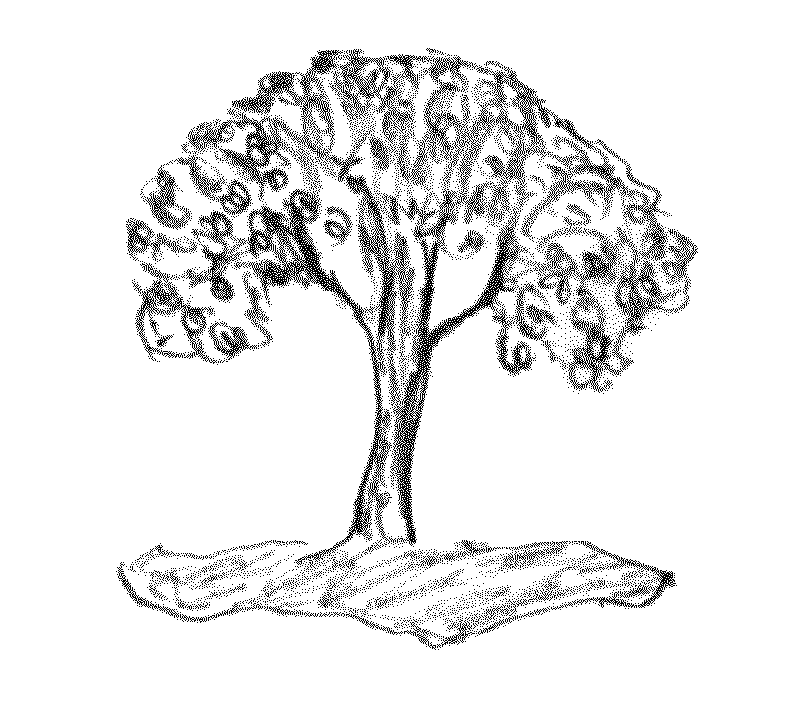
\includegraphics[width=192pt]{elm}
\end{center}

\chapter{XML, XPath, and XSLT}

When we talk about XML, we usually mean a set of conventions for representing
documents, which is derived from the Standard Generalised Mark-up Language
(SGML). SGML was designed in the late 1970s by Charles Goldfarb of IBM and
later became an ISO standard\index{standards!ISO SGML}.

This chapter provides a bit of history and a general introduction to the
XML technologies supported by RexxXML. The intent is to provide enough
information to make the rest of the guide comprehensible. You ought to
look at the reference material available from the
\href{http://www.w3.org}{World-Wide Web Consortium}\footnote{http://www.w3.org}
and other organisations such as
\href{http://www.oasis.com}{Oasis}\footnote{http://www.oasis.com} for more
depth.
As with everything else, there is a \href{http://www.ucc.ie/xml}{frequently
asked questions} list\footnote{http://www.ucc.ie/xml}.

\section{SGML}

The name Standard Generalised Mark-up Language is based on the jargon of the printing
industry. Writing
instructions to the typesetter on a manuscript is called `marking it up',
and so computer languages which provide instructions to typesetting
software became known as `mark-up' languages. Such languages typically
intersperse typesetting commands (the mark-up) with document data. Mark-up
is typically distinguished from document data by special characters
called escape characters. The bits of mark-up with their escape
characters are sometimes called `tags'.

SGML is not a mark-up language; it is a language for defining mark-up
languages. It provides conventions for the design of the mark-up
language and a formal language for describing it. In SGML-based
languages (these are called SGML applications), a document is represented as a
collection of named sections called elements. Elements can have data
associated with them in the form of named attributes, and they can have
content consisting of text and other elements. There is always one element,
sometimes called the document element or root element, which contains the
whole document. While this basic structure is shared by all SGML applications,
there's flexibility in the way the tags are represented.

The point of SGML is to separate the process of retrieving data
from a document~-- parsing the document~-- from the application-specific
processing of the data itself. Each SGML application has a set of rules called
the document type definition (DTD), which lists the elements which can be
included in the document, the attributes associated with each element, and the
structural relationship between the elements (the content model). There's a
separate, optional, set of rules, called the SGML declaration, which defines the
character set in use, the escape characters, and the SGML features required to
process the document. Given the DTD and SGML declaration, any SGML processing
software can break a document into elements (although this is not the same as
doing anything useful with the data). The SGML declaration is optional provided
the default rules are followed, but without
the DTD, it's not possible to process a document.

In its day, SGML generated a lot of excitement, to the extent that anything in
computing generates excitement. It has had some success, for instance
as the basis for the Text Encoding Initiative, and the Hypertext Mark-up
Language (HTML),
however it has not become the dominant scheme
for document representation, so far. I think
part of the problem is that it's really useful only as the basis for further
standardisation efforts\index{standards!gotta love them}. A lot of people
expected SGML to be a universal document converter, and lost interest when they
discovered it wouldn't allow them to open their WordStar documents from
WordPerfect.

Part of the problem is undoubtedly that SGML can be quite complicated.
On top of the rather simple structure I implied above, there's a morass
of details. For instance, while there's a standard set of conventions
(the `concrete reference syntax') for character encoding and escape
characters, these can be changed in the SGML declaration. For many
commentators, this fact can't be ignored, so relatively simple
statements like `{\it the ``p'' tag is represented as ``\tag{p}''}\,'
often drag in messy details that nobody cares about:
`{\it the ``p'' tag is represented as the start-tag open symbol in the current
concrete syntax, which is ``$\langle$'' in the reference concrete syntax,
followed by the letter ``p'', followed by the tag close symbol in the
current concrete syntax, which is ``$\rangle$'' in the reference concrete
syntax. In the reference concrete syntax, this appears as ``\tag{p}'',
however it is important to remember that the start-tag open and tag close symbols
might be different in a different concrete syntax}'.
That's not a quote, but it really could be. SGML also has a lot of
features to reduce the amount of typing required to create an SGML file
at the keyboard, which can make DTD-writing and document parsing more
complex.

\section{XML}

The success of the World-Wide Web propelled HTML to the forefront of
SGML applications, where it turned out to have some limitations. HTML
is well-suited for technical reports in computer science, but not
for most other kinds of documents. Sometimes reasonably, but sometimes
unreasonably, users have seen it as a barrier to providing data through
the Web.

As I understand it, HTML was not originally conceived as a formal SGML
application. Originally, it simply bore a strong resemblance to mark-up
using the default SGML character set and escape characters
(the reference concrete syntax), and was only later formalised.
As people increasingly wanted to put information on the web for which
HTML was not well suited, there was a sentiment to return to the
original approach of creating SGML-like mark-up, but without all the
complication of SGML. The result was the definition of the `Extensible
Mark-up Language', XML.

\subsection{General syntax}

XML is a simplified subset of SGML.
It removes flexibility over the escape characters and disables
SGML features which require the parser to know the document's content
model, so there's no need for the SGML declaration and XML documents can
be parsed without having a DTD. 
We
distinguish between a `valid' document\index{valid document} and a `well-formed' document\index{well-formed!document}.
A well-formed document follows a certain set of syntax rules~-- at heart, its
elements nest properly and its data is in the correct character set~--
while a valid document also has a DTD, and the mark-up of the document conforms to
the DTD. When I refer to an `XML document', I really mean
a `well-formed XML document'.

An XML document consists of comments, a document type declaration,
processing instructions, and the document element. The document element
might have data associated with it in the form of attributes, and content
consisting of other elements, text,
comments, CDATA sections, and processing instructions.
Each of the other elements might have similar sorts of content.
The remainder of this section describes these components.

\subsubsection{Comments}

Comments\index{comments!XML} start with \verb+<!--+ and end with \verb+-->+.
In between, they can contain any text other than \verb+--+. Comments are
passed to the processing program by the parser, but they shouldn't be used
in document processing, beyond preserving them when a new copy of the document
is written out. You \textit{could} use comments, but should use
processing instructions, to pass information to your application.

\begin{verbatim}
<!-- This list needs to be verified. -->
\end{verbatim}

\subsubsection{Processing instructions}

Processing instructions\index{processing instruction}\index{PI} (PI) are a general mechanism for passing information
to the program processing an XML document. They begin with \verb+<?+ and end
with \verb+?>+. In between, you must have a name which is understood by the application
to which the PI is directed, and may have any other information which is useful
to that application. Every XML document is supposed to start with a PI:
the XML declaration. It gives the version of XML
needed to process the document and optionally the character set in
which the document is encoded (the default character set is UTF-8).
The world-wide web consortium's practice is to define PIs whose syntax
is similar to elements.

\begin{verbatim}
<?xml version="1.0" encoding="ISO-8859-1"?>
 <!-- the XML declaration is supposed to start every XML file -->

 <!-- you should put version control information in a PI rather
      than a comment if it's going to be processed by software -->
<?rcsinfo $Revision: 1.21 $ ?>
\end{verbatim}

\subsubsection{Document type declaration}

The document type declaration\index{document type declaration} starts with \verb+<!DOCTYPE+ and ends with
\verb+>+. In between, it gives the name of the document element, optionally the name of a
file containing the DTD, and optionally all or part of the DTD itself. This is described in
more detail in section \ref{sec:DTD}.
In SGML, the
document type declaration is required. In XML it is optional, however the document
cannot be validated without it.

\begin{verbatim}
<!DOCTYPE adoc SYSTEM "adoc.dtd" [
  <!ENTITY regina "Regina Rexx Interpreter">
]>
\end{verbatim}

\subsubsection{Elements and attributes}

Elements are the fundamental building blocks of an XML file. All data,
excluding data in comments and PIs, is associated with some element,
either as the value of an attribute of the element or as content of the
element.
Each element is represented by its open tag, which may have
attributes associated with it, its content, and its close tag.
The open tag has the format \verb+<ename attr1='val1' attr2="val2">+
while the close tag has the format \verb+</ename>+.
Attributes consist of a name, an equals sign, and a value enclosed in either single-
or double-quotes, all of which must be present for the attribute to be
well-formed\index{well-formed!attribute}.
The element content can consist of a mixture of text and other
elements. If an element has no content, its open tag can end with
\verb+/>+\index{/>}\index{element!empty} rather than \verb+>+, in which case its close tag must be omitted.
Such an element is called an empty element.

Element and attribute names\label{page:namesyntax}\index{names!XML} start with a letter, `:', or
`\textunderscore', and continue with any number of letters, digits,
`-'s, `.'s, `:'s and `\textunderscore's. The definition of a
letter\index{letter!definition}
depends on the character set of the document. You must not start
a name with `XML' in either upper- or lower-case, and you
should not use `:' for reasons I'll get into in a moment
(actually, in section \ref{sec:namespace}).
Names in XML are case-sensitive.

All of the data in a well-formed\index{well-formed!document} XML document is contained by a single element,
the document element. An element which is content of another element is said
to be `nested'. The level of nesting is the number of open elements. Every
open tag must be matched by a close tag at the same level of nesting. You can
never have a structure
like this\index{well-formed!element content}
\begin{verbatim}
<a>data in a <b>data in a and b</a>data in b</b>
\end{verbatim}

\subsubsection{Text and entity references}

Text in an XML document is nearly-arbitrary data. When it occurs
as content of an element, it can consist of any
characters in the encoding character set, including new-lines, but excluding
\verb.<. and \verb.&.. In attribute values, text also excludes either \verb.". or
\verb.'., depending on which is used to delimit the attribute.
If the excluded values were to appear in text, the parser could confuse them with
mark-up. To avoid this, one replaces those characters with entity
references\index{entity!reference}.

Entity reference syntax is
\verb.&.{\it name}\verb.;.. This is
replaced at parse time by the entity's value, which must be declared
in the DTD unless the entity is one of the five pre-defined
entities\index{entity!pre-defined}
\verb.&lt;. (\verb.<.), \verb.&gt;. (\verb.>.), \verb.&amp;. (\verb.&.),
\verb.&apos;. (\verb.'.), or \verb.&quot;. (\verb.".).

Another approach to escaping \verb.<. and \verb.&., valid only in text which is
the content of an element,
is to enclose them in a CDATA
section. CDATA sections are opened with \verb.<![CDATA[. and closed with
\verb.]]>.. In between, any sequence of characters other than \verb.]]>.
can be typed as is.

\begin{verbatim}
<!-- using &gt; is not necessary, but seems more consistent -->
<p>A paragraph begins with &lt;p&gt; and ends with &lt;/p&gt;.</p>

<!-- You can get the same effect with CDATA -->
<p><![CDATA[A paragraph begins with <p> and ends with </p>.]]></p>

<!-- a more likely use -->
<rexx:rexx><![CDATA[
select
  when x < y then call z
  when w <= v & y = 7 then call u
  otherwise nop
  end
]]></rexx:rexx>
\end{verbatim}

Text which is inconvenient to type can be represented using character
references. A character reference\index{character reference}\index{numeric character reference}
consists of \verb.&#. followed by a decimal
character code, followed by \verb.;.. This is replaced by the unicode character
with the specified character code. The character code can be entered in
hexadecimal if the prefix is changed to \verb.&#x.. It's probably better
form to use the character reference in the definition of a general
entity, and use an entity reference in the document proper.

\begin{verbatim}
&#201;clairs are for kids. <!-- �clairs are for kids. -->
&#xc9;clairs are for kids. <!-- hex representation -->
<!ENTITY Eac "&#xc9;">     <!-- Entity declaration -->
&Eac;clairs are for kids.  <!-- Entity reference -->
\end{verbatim}


\subsection{Tree representation}

\label{sec:treerep}The general syntax describes the way XML documents are represented
for storage or
transmission. Parsing is the process of converting that format into something
which can be processed reasonably efficiently by software. Typically, we
think of the document as a tree\index{tree}. A tree is a data structure in
which data is represented as a collection of distinct nodes which have
parent/child relationships with each other\index{node}. Each node except for
one has exactly one parent. The exception has no parent, and is called the
root of the tree.

\label{page:treerep}\begin{verbatim}
<?xml version="1.0" encoding="ISO-8859-1"?>
<!-- A dreary poem -->
<poem><stanza><line>Winter has come early.</line>
         <line>The frost has iced over the empty fields</line>
         <line>and ruined the late corn.</line>
         <line>It will be a cold November.</line>
 </stanza>
 <stanza><line>Once I wondered why the world was so cruel</line>
         <line>but I have given up wondering,</line>
         <line>for who can say how the North wind blows?</line>
 </stanza></poem>
\end{verbatim}

\includegraphics{treerep}

The root of the tree is the XML document itself. All of the components listed
in the previous
section, except for attributes, have an obvious relationship either as
children of the document node or as children of one of the elements of the
document. Attributes are considered to be data associated with
their element's node. The XML declaration is treated the same way with respect
to the document node.

Each node has a type which relates to its origin in the XML document.
Elements are mapped to element nodes, text to text nodes, and so forth.
The mapping is done in such a way that the original document can be reconstructed
from the tree.

Any well-formed document\index{well-formed!document} can be parsed into such a tree, and a well-formed
document can be constructed from any such tree. RexxXML provides tools for
creating, searching, and manipulating document trees of this sort. The
approach is similar to the World-Wide Web Consortium's document object model
(DOM)\index{DOM}, but I don't claim conformance to that model, or even to
understand what conformance would entail.

\subsection{Document type definition}

\label{sec:DTD}The Document Type Definition (DTD) consists of mark-up
declarations which define the
elements, attributes, and entities which can occur in a document or a class of
documents. With a DTD, you can ensure that the set of tags used in data files
matches the set of tags your application is designed to process, give default
values to attributes, and define entity values. XML Schema, discussed in
section \ref{sec:schema}, is a more complicated mechanism for achieving the same
objectives,
with finer control. For an XML document to be valid\index{valid document}, according to the
standard, it must have an XML declaration and a document type declaration, and
it must satisfy the DTD given in the document type declaration.

The DTD is divided into two subsets. The internal subset\index{document type declaration!internal subset} is
the part of the DTD defined in the XML document itself, while the
external\index{document type declaration!external subset} subset is the part defined in a separate file.
The declarations in the internal subset supercede the
declarations in the external subset.

\subsubsection{Document type declaration}

The document type declaration itself has
three parts: the name of the document element, a reference to the external
subset of the DTD, and the whole of the internal subset. At least one of the
DTD subsets must be specified for the document to be validated\index{valid document}. Since the
document element is specified in the declaration, rather than the DTD
proper, the same DTD can be used for documents with different document
elements, for instance for a short report with just one section as well
as for longer reports with front and back matter and several sections.

The external subset can be identified in two ways, through a system identifier
or a public identifier. A system identifier\index{system identifier} is the word `SYSTEM',
followed by a URL for the file containing the DTD. A public\index{public identifier}\label{page:pubid}
identifier is introduced by the word `PUBLIC', which is followed by the public
identifier of the DTD, and sometimes by a URL for the file.
Public identifiers are used to define formally published DTDs. The format is
something like `-//', the name of the organisation which published the DTD,
`//', the name of the DTD, `//', and the language code of the DTD. For DTDs
which have been approved by ISO, the `-//' is replaced by `+//'.

\begin{verbatim}
<!-- declaration with no DTD -->
<!DOCTYPE mydoc>
<!-- declaration with public identifier for DTD -->
<!DOCTYPE mydoc PUBLIC "-//my organisation/mydoc/en">
<!-- declaration with system identifier for DTD -->
<!DOCTYPE mydoc SYSTEM "mydoc.dtd">
\end{verbatim}

The internal subset is enclosed in brackets ([\,]) at the end of the document
type declaration. Most documents don't have one, but the ones that do use it to define
document-specific entities, or to make local modifications to the content
model, not that that's a good idea. The internal subset can also be used
to define parameter entities which in turn can influence conditional
inclusion in the external subset.

\begin{verbatim}
<!-- declaration with internal subset only -->
<!DOCTYPE mydoc [ <!ELEMENT mydoc ANY> ]>
<!-- declaration with external and internal subsets -->
<!DOCTYPE mydoc PUBLIC "-//my organisation/mydoc/en" "mydoc.dtd" [
   <!ENTITY % myextras "|pps">
   <!ELEMENT pps (#PCDATA)*>
]>
\end{verbatim}

There are some differences in the way the external and internal subsets
are specified, but
in either case, the DTD is made up of comments, and declarations for elements,
attributes, entities, and notations.
Each type of declaration is described in the remainder of this section.

\subsubsection{Element declaration}

An element declaration\index{element!declaring in DTD} consists of \verb+<!ELEMENT+, the
element name ($n$), the content model for $n$, and \verb+>+.
The content model lists the types of data which are permitted
as content of $n$, with their order and cardinality (the
number of times the data may appear). It can be either of the
words `EMPTY' (meaning $n$ cannot have any content) or `ANY'
(meaning $n$ has no constraints on its content), or it can be
more complicated than that. There are two kinds of more-complicated
content models, element content models, and mixed content models. The
rules for each are similar but different, so I'll gloss them over
separately.

In an element content model, anything that appears as content of $n$
must be an element itself, it must be one of the elements listed in
the content model, and all the content must be in the order specified by
the content model.  Any text that appears as a descendant of
$n$ must be included in some other element.

The components of the content model are
elements, sequences, and sets. An element is
represented by its name.
A sequence is a list of components, separated by commas (,), and surrounded by
parentheses ((\,)).
A set is a list of components, separated by pipes (|), and surrounded by parentheses. 
Any component can be followed by a question mark (?), meaning that the component may occur
zero or one time, an asterisk (*), meaning that the component may occur zero or many
times, or a plus sign (+), meaning that the component must occur at least one time and may
occur many more times. The element content model itself is either
a sequence, possibly with only one element, or a set, and may be
followed by a question mark, asterisk, or plus sign.

Mixed content models are similar to what I've called sets in my description of
element content models. A mixed content model consists of `\#PCDATA' and
a list of element names, separated by pipes. \#PCDATA must come first.
The entire list must be enclosed in parentheses, and must be followed
by an asterisk. PCDATA means parsed character data, which is ISO's way of saying
text. There's no way to allow an element to have text content and
enforce any kind of structure on the rest of the content, apart from
restricting the elements which can be used.

In the hopes that all of that will become clear, here are some examples
of element declarations\index{hoping to avoid confusion}.

\begin{verbatim}
<!ELEMENT doc (front,sec+,back?)>
<!ELEMENT front (titlepage,lcdata,toc?,sec*)>
<!ELEMENT sec (head,(par|figure)+)>
<!ELEMENT back (sec*,index?)>
<!ELEMENT titlepage (title,author+,publisher)>
<!ELEMENT lcdata (title,(author,dates?)+,etc+)>
<!ELEMENT toc EMPTY>
<!ELEMENT name (#PCDATA)*>
<!ELEMENT author (#PCDATA)*>
<!ELEMENT publisher (#PCDATA)*>
<!ELEMENT dates (#PCDATA)*>
<!ELEMENT etc (#PCDATA)*>
<!ELEMENT head (#PCDATA|b|i)*>
<!ELEMENT par (#PCDATA|b|i|ind)*>
<!ELEMENT figure EMPTY>
<!ELEMENT b (#PCDATA)*>
<!ELEMENT i (#PCDATA)*>
<!ELEMENT ind (#PCDATA)*>
<!ELEMENT index EMPTY>
\end{verbatim}

This describes the structure of a document, which is enclosed by the
`doc' element. Here are text descriptions of the content models for
selected elements:
 `doc' has element content, consisting of a sequence of
elements. It must start with a `front', which must be followed by
at least one `sec', but possibly more than one (due to +), and it might end
with a `back', but that's optional (due to ?).
`sec' is slightly more complicated: it must start with `head', and that
must be followed by at least one of `par' or `figure'. There can be any
number of additional `par's and `figure's, in any order. `head' and `par' have mixed content. They can consist of any
combination of text, or the `b', `i', or (par only) `ind' elements. `figure' is an
example of an empty element~-- all of its data presumably comes from
attributes which I haven't shown.
`lcdata' is a required part of the front matter, and must start with
one instance of `title'. `author' and optionally `dates' must occur
at least once, and are repeated in sequence for
each author. There's additional required cataloguing information. It would normally
be spelled out better, but I'm not a librarian so I've stuck it in a single element called
`etc', which must occur at least once, and may occur many times.
`title', `author', `dates', and `etc' can each contain text only.

Here's a document that satisfies that DTD:
\begin{verbatim}
<doc><front><titlepage><title>Example</title><author>Me</author>
     <publisher>VW Press</publisher></titlepage>
     <lcdata><title>Example</title><author>Me</author>
       <etc type="publisher">VW Press</etc></lcdata>
     <sec id="s1"><head>Acknowledgements</head>
       <par>I'm really very grateful.</par></sec>
     </front>
     <sec><head>A heading</head>
       <par>I hope this is helpful.</par></sec>
</doc>
\end{verbatim}

Note that everything in the example except for the `sec' marked with id s1 is required by
the DTD, although obviously the content could be more interesting. There
could be more `sec's providing useful information, more authors,
back-matter and so on, but not much less than what's shown here.

\subsubsection{Notation declaration}

Notations are used to define the format of data and to identify
applications which can process the data. The notation name can be
associated with processing instructions, attributes, or entities. The
declaration syntax is \verb.<!NOTATION. {\it name} {\it
identifier}\verb.>., where {\it identifier} is either a system or public
identifier, as defined for the document type declaration on page \pageref{page:pubid}.
For instance, we could define a processor for the rcsinfo PI mentioned
earlier as
\begin{verbatim}
<!NOTATION rcsinfo SYSTEM "parsercsinfo">
\end{verbatim}
\noindent There are publicly registered notations defined by diverse
organisations such as ISO. I'm not sure of the best way to look them up.
In some cases, people use MIME application types.
Notations don't seem to be commonly used but I've
mentioned them first because they come up in the descriptions of both
attributes and entities.

\subsubsection{Attribute declaration}

Attributes are pieces of data associated with elements. In designing
XML mark-up, one challenge is deciding which data should be represented
as an attribute and which should be represented as content of the element.
Attributes have names and cannot be repeated for the same element,
so an attribute is a good choice for something which can be given
a name and of which there can be only one per element. Attributes are
also a good choice for data used to describe or identify an element,
as opposed to the element's data proper {\it e.g.,} the HTML `id'
attribute, which assigns a name to its element. Structured data, on the
other hand, should generally be represented as content.

Attributes are declared\index{attribute!declaring in DTD} in a list, which includes all the attributes for the
element in question. The syntax is \verb.<!ATTLIST. {\it element}
{\it name${}_1$} {\it type} {\it default}\dots {\it name}$_n$\dots
\verb.>.. Each attribute normally appears on its own line, and includes
the type of the attribute and a default value. The
{\it name}s follow the conventions for names given on page
\pageref{page:namesyntax}. {\it Default} indicates the value to assign to the attribute
if the attribute is not included in the mark-up. It must be one of
`\#IMPLIED', meaning that the processing application should know how to deal
with it, `\#REQUIRED', meaning that the attribute must be included in the
mark-up for this element, or a quoted string, which is taken as a literal default.
The string can
be prefixed with `\#FIXED', which means that if the attribute is
specified, its value must match the default. This is a fun way to
frustrate users, but has limited additional value.
{\it Type} can be one of the values given
in the table:

\label{page:attrtype}\begin{longtable}{lp{10cm}}
\it Type&\it Meaning\\
\endhead
CDATA&The attribute can contain nearly arbitrary text, and entity references
will be replaced by the correct values;\\
ID&The value must follow the conventions for names, and it must
be unique for all ID attributes in the document (ID defines a unique identifier).
There can be no more than one attribute with ID type on any one element. The
default value must be \#IMPLIED or \#REQUIRED;\\
IDREF&The attribute must match the name of an ID attribute somewhere in the document;\\
IDREFS&A space-delimited list of IDREF;\\
ENTITY&The attribute must match the name of an unparsed entity defined for this
document;\\
ENTITIES&A space-delimited list of ENTITY;\\
NMTOKEN&The attribute value follows the conventions for names, except that it
can start with digits, meaning it could be a number. You still have to put
quotes around the value;\\
NMTOKENS&A space-delimited list of NMTOKENS;\\
NOTATION ($n_1|\dots|n_k$)&The attribute value must match one of the $n_i$, each
of which must be the name of a NOTATION defined for the
document. The value of the attribute indicates the way the element content should
be interpreted. Only one NOTATION attribute can be specified per element. The
element must have content ({\it i.e.}, can't be declared EMPTY);\\
($n_1|\dots|n_k$)&Each $n_i$ follows the rules for NMTOKEN ({\it i.e.},
they're names or numbers). The value can be any of the $n_i$.\\
\end{longtable}

Most of the time, people use CDATA or an enumeration (the last option in the
table) for attribute types. ID and IDREF can be useful in conjunction with
XPath, though, and NOTATION could be helpful when encoding data such as
pictures.

\begin{verbatim}
<!-- from the previous example, we had an id attribute on the
     sec element -->
<!ATTLIST sec id ID #IMPLIED>

<!-- not from the previous example, you might associate author
     information with the element as attributes. The content
     would then be free to hold a list of titles or something
     like that -->
<!ATTLIST author name CDATA #REQUIRED
                 phone NMTOKEN #REQUIRED
                 e-mail CDATA #REQUIRED>

<!-- an in-line image could be in one of several formats, which
     might be identified using notations -->
<!NOTATION jpeg PUBLIC "-//my organisation//image jpeg//en">
<!NOTATION tiff PUBLIC "-//my organisation//image tiff//en">
<!NOTATION png  PUBLIC "-//my organisation//image png//en">

<!ATTLIST img id ID #IMPLIED
              format NOTATION (jpeg|tiff|png) "jpeg">
\end{verbatim}

These might be used to create this fragment of an XML document. Note
that the content of `img' must be valid text. The easiest way to
ensure this for arbitrary binary data is to use MIME base-64 encoding,
which is a mapping from arbitrary binary data to letters, numbers, +, and
/. The nature of the encoding used has to be determined by whoever is
specifying the notation (in this case, we're pretending it's me), but
there has to be something since just sticking JPEG-encoded data in the 
middle of an XML document will introduce illegal characters and result
in a parse error.\index{hoping to avoid confusion}

\begin{verbatim}
<author name="Patrick TJ McPhee" phone="1-416-422-2034"
        e-mail="ptjm@interlog.com"/>
<img>/9j/4AAQSkZJRg.../2Q==</img>
\end{verbatim}

\subsubsection{Entity declaration}

\label{sec:entdecl}It's difficult to start a sentence with `an entity is', because there
are a few kinds of entities, and the XML specification applies the term
to a few things that aren't declared as entities, so that even my
broadest attempt `an entity is a named piece of data' isn't strictly
correct. It's probably for the best, since it forces me me to abandon
the boring, formulaic style into which I've degenerated and write something
fresh and dynamic. Perhaps I'll do that later.
Apart from the document itself and the external subset of the
DTD, an entity {\it is} a named piece of data. There are five pre-defined
entities, and others can be defined in the DTD using entity declarations.

As long as you ignore the document itself and the external subset of the
DTD, entities can be divided into two, along several axes.\index{entity!divided into two types} There are
`general' entities and `parameter' entities, `internal' entities and
`external' entities, `parsed' entities and `unparsed' entities.
The entity declaration sets up an association between a name and
some data. An internal entity includes the data in the declaration
itself, while an external entity uses a system or public identifier to
refer to data in an external file. Parsed entities can be used in entity
references. The references are replaced by the entity's data, and then
parsed as if the text had appeared in the document. Unparsed entities
cannot be used that way~-- their names can be the value of an attribute
of type ENTITY, and then it's up to the application to decide what to do
with them. A general entity is for use within an XML document, while a
parameter entity is for use within a DTD.

The syntax of a general entity declaration\index{entity!declaration} is \verb.<!ENTITY. {\it name}
{\it value} \verb.>.. A parameter entity declaration is almost the
same: \verb.<!ENTITY %. {\it name} {\it value} \verb.>.. In both cases,
{\it name} is a name following the conventions whose explication is one of the principal
sources of joy on page
\pageref{page:namesyntax}, while {\it value} is either a bunch of text in
quotes (internal entity), a system or public identifier (external
entity), or a system or public identifier plus the name of a notation,
in the form \verb.NDATA. {\it name} (unparsed entity).

\begin{verbatim}
<!-- an internal parsed general entity -->
<!ENTITY product "ACME Rocket Launcher">

<!-- an external parsed general entity. The file disclaimer.xml
     could contain several paragraphs of text, much of it in upper-case -->
<!ENTITY disclaimer SYSTEM "disclaimer.xml">

<!-- an unparsed general entity, which must be external -->
<!ENTITY logo SYSTEM "vw.png" NDATA png>
\end{verbatim}


As noted earlier, the format for an entity reference\index{entity!reference} in an XML document
is \verb.&.{\it name}\verb.;.. This can appear in an attribute value
or in mixed element content.
After the entity replacement is
done, parsing restarts from the beginning of the replacement text. The
text can contain anything which could appear as a literal part of the
document at that location, including references to other entities and
element start and end tags. 
There are a few restrictions\index{well-formed!entity references}. External entities are not allowed in
attribute values. Any element start and end tags must match up, so that
failure to replace the entity reference does not result in tag
mismatches. Finally, you need to ensure that the entity content is
valid for the context in which the entity is used.

The data in an external entity does not have to be in the same character
set as the data in the document. External entities can start with a `text
declaration', which looks exactly like the XML declaration, and serves
exactly the same purpose. The encoding attribute of this declaration
should specify the character set used to encode the data.

Parameter entities\index{entity!parameter}\index{entity!use in DTD} work
much the same way as general entities, but are valid only within the DTD.
The format for a parameter entity reference is \verb.%.{\it
name}\verb.;.. In the internal subset of the DTD, parameter entity
references must contain complete mark-up declarations, which limits
their usefulness a bit\index{well-formed!parameter entity}.
When used in the external subset, or in an external
parameter entity file, parameter entity references are subject to
less severe well-formedness restrictions and can appear within
mark-up declarations.
It's common to use parameter entities to define
repeated portions of element content models, or repeatedly used
attributes. For instance, if I'd read to the end of the section
before constructing my first example, I could have written

\begin{verbatim}
<!ENTITY % text "#PCDATA|b|i">
<!ELEMENT head (%text;)*>
<!ELEMENT par (%text;|ind)*>
\end{verbatim}

\noindent keeping in mind that that would not work in the internal subset. 

External parameter entities provide a method for sharing common definitions between
completely separate DTDs. One document's DTD could be another
document's external parameter entity.

You can also use parameter entities to control conditional
inclusion\index{conditional inclusion}
within a DTD. If you have \verb.<![IGNORE[.{\it text}\verb.]]>. in the
external subset of a DTD, {\it text} will be ignored. If you instead have 
\verb.<![INCLUDE[.\textit{text}\verb.]]>., {\it text} will be included. {\it Text}
can consist of mark-up declarations, comments, and processing
instructions. The literal text `IGNORE' or `INCLUDE' can be replaced by
a parameter entity, which means alternate versions of the DTD can be
invoked simply by setting a parameter entity appropriately in the
internal subset.

\begin{verbatim}
<!-- in the external subset -->
<![%book;[<!ELEMENT front (titlepage,lcdata,toc,sec*)>]]>
<![%paper;[<!ELEMENT front (titlepage,toc?)>]]>

<!-- in the internal subset -->
<!ENTITY % book "IGNORE">
<!ENTITY % paper "INCLUDE">
\end{verbatim}

DTDs are useful, but one of the glories of XML is that they're not required.
You don't have to worry about them when you're experimenting with XML-based
solutions, but you should consider creating a DTD whenever you define a
document structure which you intend to publish or simply use for a long time.

\subsection{Name-spaces}

\label{sec:namespace}One goal of XML was to allow mark-up to be extended in modular ways.
For instance, there are very many different document structures, each
of which could be given its own DTD, but within that structure, the
definition of building-blocks such as paragraphs and tables could be
the same. One difficulty with importing definitions from one DTD into
another is that some tags might have been used in more than one DTD.  Such a
duplication is sometimes called a name-space collision. XML Name-Spaces
are an effort to address this issue.

A name-space is simply a unique URL which has been set aside by a
document designer to distinguish some set of tags. Within a document,
the name-space is associated with a name called the name-space
prefix\index{name-space!prefix}, and any element or attribute from the
set of tags has this prefix and a colon (:) prepended to it. The syntax
rules for the prefix are the same as for any other name, except that
it must not include a colon. Usually, the name-space prefix consists
of a small number of letters.
Name-spaces can be used on both element and attribute names. I assume
they can also be used for notations and entities, but I don't recall
ever having seen it done.

Software processing the document decodes the prefixed name into a URL
and a tag name, and it can use these to determine the appropriate
processing for the elements in question. Note that this processing
is based on the URL and not the prefix. With the exception of
the predefined name-spaces mentioned in the next paragraph, the actual
value of the prefix is not supposed to be relevant.

Name-space prefixes beginning with `xml' are reserved for use in future
extensions to the language. In particular, the `xml' prefix is associated
with the attributes `lang' and `space', which XML processors are all
supposed to understand\footnote{xml:lang\index{xml:lang} specifies the document's
language using the language codes defined in RFC 1766\index{RFC 1766} (en-CA for Canadian English,
fr-CA for Canadian French, de for German independent of country, etc).
xml:space\index{xml:space} with the value `preserve' indicates that white-space
should be preserved in contexts where text is not permitted.}
Other name-space prefixes are declared using an attribute whose name-space is `xmlns'
and whose name in that space is the prefix being declared. The value of
the attribute is the name-space's URL.
\begin{verbatim}
<text xmlns:pt="http://www.interlog.com/~ptjm/mytables">
 <pt:table>
  <pt:row><pt:col>1,1</pt:col><pt:col>2,1</pt:col></pt:row>
  <pt:row><pt:col>1,2</pt:col><pt:col>2,2</pt:col></pt:row>
 </pt:table>
</text>
\end{verbatim}

In the example, I declare a name-space with prefix `pt', which is
associated with a URL. In this case, the URL doesn't refer to an actual
resource, but it's either unique, or whoever else used it to define
a name-space really had no business doing so. You don't have to
use an HTTP address for the URL, but it's common to take advantage
of the uniqueness of machine addresses. The name-space declaration
has to appear on either the element where the prefix is used, or on
one of the elements that contains it. It's common to put all the
name-space declarations for a document on the document element
itself.

It's also possible to declare a name-space which doesn't use a prefix,
which is called a default name-space\index{name-space!default}.
This is equivalent to the previous example:
\begin{verbatim}
<text>
 <table  xmlns="http://www.interlog.com/~ptjm/mytables">
  <row><col>1,1</col><col>2,1</col></row>
  <row><col>1,2</col><col>2,2</col></row>
 </table>
</text>
\end{verbatim}

\noindent All the table, row, and col elements are associated
with the same name-space as the pt:table, pt:row, and pt:col elements
of the previous example. The text element is not in this case because
it occurs outside the scope of the default name-space declaration,
and in the previous case because it doesn't have a prefix.

When writing a DTD for XML mark-up that uses name-spaces, you have to
include the imported elements, with their name-space prefix, in the
DTD. For instance, I might have
\begin{verbatim}
<!ELEMENT pt:table (pt:row+)>
<!ELEMENT pt:row (pt:col+)>
\end{verbatim}

This is a bit pointless, though~-- what's the good of the prefix if it
needs to be specified in the DTD? To get around the problem, specify the
prefix as a parameter entity. The entity value can then be changed in the
internal subset if necessary.

\begin{verbatim}
<!ENTITY % pt "pt:">

<!ELEMENT %pt;table (pt:row+)>
<!ELEMENT %pt;row (pt:col+)>
\end{verbatim}

\subsection{Schemas}

\label{sec:schema}As the name says, DTDs are for defining the structure of
documents. There's a need for data validation, in addition to structural
validation, for applications which use XML as a data exchange protocol. A
schema definition is an XML document whose elements are used to define the
elements, attributes, and notations of another document. Schemas allow precise
specification of data types, including value checking, record structures, and
precise control over cardinality, for both element content and
attribute values.

The schema proper is called an XML Schema Definition, and is often
stored in a file with the extension .xsd. Documents based on a schema
are called, albeit rarely, XML Schema Instances. To specify in a
document the name of the schema to which it conforms, one must include
an attribute from the schema instance name-space:

\begin{verbatim}
<data xmlns:xsi="http://www.w3.org/2001/XMLSchema-instance"
      xsi:schemaLocation="dataDefinition.xsd">
 ...
</data>
\end{verbatim}

A brief but comprehensive description of schemas would take forty or fifty pages,
and they wouldn't be the most interesting forty or fifty pages written
this year. I'm going to give an overview touching on the
most important elements. I will use the name-space prefix xs:, which should be
associated with http://www.w3.org\slash 2001\slash XMLSchema, for schema elements.

XML Schemas can define elements, attributes, notations, and data types.
There are facilities for deriving element and type definitions
from previously defined elements and types, and for accessing externally
defined schemas. There's no mechanism for defining entities.
Each of the things schemas can define has one or more elements associated
with it.

\paragraph{Annotations}

Schemas can be documented using the xs:annotation\index{xs:annotation} element. It can appear
at the start of the content of essentially every element in
the schema model, other than xs:annotation itself. Its content is made up of xs:documentation\index{xs:documentation}\index{comments!XML Schema} and
xs:appinfo\index{xs:appinfo} elements, which correspond to XML comments and XML processing
instructions, respectively. xs:documentation is meant for humans to read,
while xs:appinfo is meant for programs to process.

\paragraph{Structure}

The document element for a schema is xs:schema\index{xs:schema}. It contains all the
definitions for the schema. I'll mention three of its attributes:
`xml:lang' specifies the language of the schema, `targetNamespace' gives the
name-space URL\index{name-space!in XML Schema} for the elements defined in the schema, and `version' gives
the version of the schema document. xs:schema and every other element
in the schema document can have an `id' attribute, which allows
other documents to link to parts of the schema.

\paragraph{Elements and attributes}

Elements are defined using xs:element\index{xs:element}\index{element!declaring in XML Schema}. Important attributes are `name',
which gives the name of the element, `type', which names its data type,
and `default', which is the default value.
If the `type' is specified, it's the name of a type which is either pre-defined
or defined by a type definition in this schema. Otherwise, except in one
case I'll get to momentarily, the data type definition appears as
content of xs:element.

xs:attribute\index{xs:attribute}\index{attribute!declaring in XML Schema} defines an attribute. Its attributes are the same as the
ones listed above for xs:element, except that xs:attribute also has `use',
which takes the values `prohibited', `optional',
and `required', which indicates whether the attribute can or must appear
in the instance document.
As with xs:element, the type can be specified either using the
`type' attribute or as content of the xs:attribute element.

\paragraph{Data types}

Data types are divided into simple types, which are all essentially text with
restrictions on the kind of data that can appear, and complex types, which are
all essentially content models. Attributes can have only simple types, while
elements can have either kind of type. Type definitions can appear stand-alone
(in which case they must be given a name) or as content of an element or
attribute definition. Type definitions which are defined as element or
attribute content are sometimes called
anonymous types.
\index{data types!simple}
\index{data types!complex}
\index{data types!anonymous}

All simple types are based on a set of so-called primitive data types
defined in the XML Schema specification.
A simple type\index{data types!simple} restricts another simple type by setting
properties, or it extends one or more simple types by creating either a
list of elements of one type, or a union of the value sets of two or more types.
Simple types are defined using xs:simpleType\index{xs:simpleType}, which
has the attributes `name', which names the type, and `final', which
prevents type type from being extended through `restriction', `extension',
or both.
Derivations are defined using the elements xs:restriction,\index{xs:restriction}
xs:list\index{xs:list}, and xs:union\index{xs:union}.

\index{data types!predefined in XML Schema}
Important predefined types are string, decimal (arbitrary-precision numbers),
integer (the integer subset of arbitrary-precision numbers),
and dateTime (date/time). There are also types such as int and float, which
are described in terms of well-known numeric binary types. Note that while
they are described in terms of binary types, the values are always text. If
`7' is represented as an `int', the hex value of the representation is `37',
and not `00000007'. There is an immense list of binary-inspired text types
which one might take as further evidence that XML is the anti-Rexx.
If you need to use a type other than string or decimal, you need to
acquire a proper reference manual for XML Schema.

xs:restriction\index{xs:restriction} creates a new type by defining a subset
of the values of another type. Its attribute is `base', which gives the name
of the type which is being restricted.
Data type restrictions are defined in terms of standardised properties
called facets. Each facet is its own element with an attribute
called `value', which appear as content of xs:restriction. Significant facets,
whose names are hopefully
\index{xs:length}%
\index{xs:minLength}%
\index{xs:maxLength}%
\index{xs:minInclusive}%
\index{xs:maxInclusive}%
\index{xs:pattern}%
\index{xs:enumeration}%
self-explanatory, are `length', `minLength', `maxLength', `minInclusive',
`maxInclusive', `enumeration', and `pattern'. More than one xs:enumeration
can be included in an xs:restriction. The set of all the `value'
attributes is the set of allowable values for the type.
The value of `pattern' is a regular expression
which matches all valid data of the given type.
I'm not going to document the regular expression syntax here. I'll note that
`c[ao]t' matches `cat' and `cot', `colou?r' matches `color' and `colour',
`a$\{2,3\}$' matches `aa' or `aaa', `a.c' matches `a' followed by any
character, followed by `c', and `(true|false)' matches `true' or `false'.

Most sensible people don't want a lot of trouble, so, short of avoiding
Schema definitions like a Spice Girls reunion, they define their
data to use the standard types with simple restrictions. For instance,
Canadian Social Insurance Numbers are 9-digit numbers which must follow
a particular formula. Oops, Schema has no standard way of expressing the
formula\footnote{Additional validation instructions can be specified using
xs:appinfo, but they are application-specific.}, but we can be happy putting
in the length limitation:

\begin{verbatim}
<xs:simpleType name="SIN">
 <xs:restriction base="xs:integer">
   <xs:length value="9"/>
 </xs:restriction>
</xs:simpleType>
\end{verbatim}

Simple types can also be extended by combining two or more types
using xs:union\index{xs:union}. For instance, if we wanted to match Canadian postal codes,
we would use this type:

\begin{verbatim}
<xs:simpleType name="CanadaCode">
 <xs:restriction base="xs:string">
   <xs:pattern value="[A-Z][0-9][A-Z] [0-9][A-Z][0-9]"/>
 </xs:restriction>
</xs:simpleType>
\end{verbatim}

\noindent whereas an American zip code matches this type:

\begin{verbatim}
<xs:simpleType name="USCode">
 <xs:restriction base="xs:string">
   <xs:pattern value="[0-9]{5}(-[0-9]{4})?"/>
 </xs:restriction>
</xs:simpleType>
\end{verbatim}

\noindent and a UK postal code matches this type (I think):

\begin{verbatim}
<xs:simpleType name="UKCode">
 <xs:restriction base="xs:string">
   <xs:pattern value="[A-Z]{2}[0-9]{1,2} [0-9]{1,2}[A-Z]{2}"/>
 </xs:restriction>
</xs:simpleType>
\end{verbatim}

\noindent If we want to match any of those codes, we can combine them in a union:

\begin{verbatim}
<xs:simpleType name="CUKSCode">
 <xs:union>
  <xs:simpleType>
   <xs:restriction base="CanadaCode"/>
  </xs:simpleType>
  <xs:simpleType>
   <xs:restriction base="USCode"/>
  </xs:simpleType>
  <xs:simpleType>
   <xs:restriction base="UKCode"/>
  </xs:simpleType>
 </xs:union>
</xs:simpleType>
\end{verbatim}

Finally, if we want to create a list of some atomic type (a type which
doesn't allow spaces, such as the USCode above), we can use the xs:list\index{xs:list}
element

\begin{verbatim}
<xs:simpleType name="USCodeList">
 <xs:list itemType="USCode"/>
</xs:simpleType>
\end{verbatim}

Simple types can be associated with elements or attributes either
by name or by having their definition as content of the xs:element\index{xs:element} or xs:attribute\index{xs:attribute}
element. Given the amazing type definitions we've already seen we could
define a postcode attribute
\begin{verbatim}
 <xs:attribute name="postcode" type="CUKSCode" default="M4K 2T1"/>
\end{verbatim}

We might repeat the SIN definition to get a SIN element

\begin{verbatim}
<xs:element name="SIN">
 <xs:simpleType>
  <xs:restriction base="integer">
    <xs:length value="9"/>
  </xs:restriction>
 </xs:simpleType>
</xs:element>
\end{verbatim}

xs:complexType\index{xs:complexType}\index{element!declaring in XML Schema}
is used to define content models. The attributes you need to know about are
`name' (the type name), and `mixed' (true or false -- whether the type
is a mixed content model).
The definitions are
similar to those of DTDs, but provide more control
over certain relationships.

In section \ref{sec:DTD}, I talked about elements, sets, and sequences.
These are represented in schemas by the elements xs:element, xs:choice,
and xs:sequence, respectively.

Within an xs:complexType,
xs:element\index{xs:element} has additional useful attributes, beyond
what I mentioned before. `ref' gives the name of another element, and can be used
in place of `type' to indicate that this element has the same type as
that other element.
`minOccurs' and `maxOccurs', indicate the
cardinality of the element with finer control than DTDs permit.
The value of `minOccurs' can be any non-negative integer, and the
value of `maxOccurs' can be any integer greater than `minOccurs',
or the string `unbounded'.

\begin{verbatim}
<!ELEMENT shift (forward+, defence+, goalie)>
\end{verbatim}

\indent can be defined as

\begin{verbatim}
<xs:element name="shift">
  <xs:complexType>
    <xs:sequence>
      <xs:element minOccurs="3" maxOccurs="3" ref="forward"/>
      <xs:element minOccurs="2" maxOccurs="2" ref="defence"/>
      <xs:element ref="goalie"/>
    </xs:sequence>
  </xs:complexType>
</xs:element>
\end{verbatim}

\noindent (assuming forward, defence, and goalie are defined elsewhere in
the schema). Which says that a shift consists of three forwards,
two defencemen, and a goalie. The same thing can be expressed exactly
in a DTD simply by repeating each element name the required number
of times, but it's more error-prone, and there exists
some value of `maxOccurs' where using Schema will be more succinct.

xs:choice\index{xs:choice} and xs:sequence\index{xs:sequence} have the
attributes `minOccurs' and `maxOccurs'. The content can be any number
of xs:choice, xs:sequence, or xs:element elements. For instance, we
can allow for a shift with the goalie pulled:

\begin{verbatim}
<xs:element name="shift">
  <xs:complexType>
    <xs:choice>
      <xs:sequence>
        <xs:element minOccurs="3" maxOccurs="3" ref="forward"/>
        <xs:element minOccurs="2" maxOccurs="2" ref="defence"/>
        <xs:element ref="goalie"/>
      </xs:sequence>
      <xs:sequence>
        <xs:element minOccurs="4" maxOccurs="4" ref="forward"/>
        <xs:element minOccurs="2" maxOccurs="2" ref="defence"/>
      </xs:sequence>
    </xs:choice>
  </xs:complexType>
</xs:element>
\end{verbatim}

\noindent which is equivalent to

\begin{verbatim}
<!ELEMENT shift ((forward,forward,forward, defence, defence, goalie)|
                 (forward,forward,forward,forward, defence, defence)) >
\end{verbatim}

Attributes defined using an xs:attribute\index{xs:attribute} element can be added to an element or complex type
by listing them alongside the complexType components. Since hockey teams
often have set lines and defensive pairings, we might put in attributes
as a short-hand for times when a set line was on the ice:

\begin{verbatim}
<xs:element name="shift">
  <xs:complexType>
    <xs:choice minOccurs="0">
      <xs:sequence>
        <xs:element minOccurs="3" maxOccurs="3" ref="forward"/>
        <xs:element minOccurs="2" maxOccurs="2" ref="defence"/>
        <xs:element ref="goalie"/>
      </xs:sequence>
      <xs:sequence>
        <xs:element minOccurs="4" maxOccurs="4" ref="forward"/>
        <xs:element minOccurs="2" maxOccurs="2" ref="defence"/>
      </xs:sequence>
    </xs:choice>
    <xs:attribute name="lineno" type="xs:integer"/>
    <xs:attribute name="defencepairno" type="xs:integer"/>
  </xs:complexType>
</xs:element>
\end{verbatim}

\noindent So far as I know, there's no way to indicate that the content
is optional only if `lineno' and `defencepairno' are specified. If you
need that sort of control, you either need to build it in to your
application or use elements to hold the data.

We can define mixed content elements by setting the `mixed' attribute of
xs:complexType to `true' and defining the content as an xs:choice.
Suppose we wanted to represent a forward by a player id, and to specify
that the id had to match the id of a player element from the same document.
We could allow either the syntax \tag{forward}\tag{id}Mc0270\tag{/id}\tag{/forward}
or the syntax \tag{forward}Mc0270\tag{/forward} with this definition

\begin{verbatim}
<xs:element name="forward">
  <xs:complexType mixed="true">
    <xs:choice>
      <xs:element name="id" type="xs:IDREF"/>
    </xs:choice>
    <xs:attribute name="wing" default="centre">
      <xs:simpleType>
        <xs:restriction base="xs:string">
          <xs:enumeration value="left"/>
          <xs:enumeration value="right"/>
          <xs:enumeration value="centre"/>
        </xs:restriction>
      </xs:simpleType>
    </xs:attribute>
  </xs:complexType>
</xs:element>
\end{verbatim}

\noindent but that doesn't place any constraint on the text content. We
can place constraints on the text constant by defining a simple type, but
that doesn't allow us to define attributes for the element.

To allow typed text content with attributes, there's an element called
xs:simpleContent\index{xs:simpleContent}. It derives complex types from simple
types, using the same extension mechanism as we use to derive simple
types from other simple types.

\begin{verbatim}
<xs:element name="forward">
  <xs:complexType>
    <xs:simpleContent>
      <xs:extension base="xs:IDREF">
        <xs:attribute name="wing" default="centre">
          <xs:simpleType>
            <xs:restriction base="xs:string">
              <xs:enumeration value="left"/>
              <xs:enumeration value="right"/>
              <xs:enumeration value="centre"/>
            </xs:restriction>
          </xs:simpleType>
        </xs:attribute>
      </xs:extension>
    </xs:simpleContent>
  </xs:complexType>
</xs:element>
\end{verbatim}

We can define empty elements with attributes
by leaving most of the type definition out:

\begin{verbatim}
<xs:element name="author">
 <xs:complexType>
   <xs:attribute name="name" type="xs:string"/>
   <xs:attribute name="phone" type="naphone"/>
   <xs:attribute name="e-mail" type="xs:string"/>
 </xs:complexType>
</xs:element>
\end{verbatim}

\paragraph{Attribute and element groups}

Commonly, groups of attributes are repeated for several elements. In a
DTD, the attribute definitions could be assigned to a parameter entity,
and an entity reference added to the various ATTLISTs: 

\begin{verbatim}
<!ENTITY % person-parms name CDATA #REQUIRED
                        number CDATA #REQUIRED
>
                       <!-- ... -->
<!ATTLIST tinker %person-parms; %tinker-parms;>
<!ATTLIST tailor %person-parms; %tailor-parms;>
<!ATTLIST soldier %person-parms; %soldier-parms;>
<!ATTLIST sailor %person-parms; %sailor-parms;>
\end{verbatim}

\noindent With schemas, attributes are grouped in an
xs:attributeGroup\index{xs:attributeGroup}
element, which has attribute `name', and a reference to the group takes their place
in the element or type definition:

\begin{verbatim}
<xs:attributeGroup name="person-parms">
  <xs:attribute name="name" type="xs:string"/>
  <xs:attribute name="number" type="xs:integer"/>
</xs:attributeGroup>
                       <!-- ... -->
<xs:element name="tinker">
  <xs:complexType>
    <xs:attributeGroup ref="person-parms"/>
    <xs:attributeGroup ref="tinker-parms"/>
  </xs:complexType>
</xs:element>
                       <!-- ... -->
\end{verbatim}

In a similar vein, repeated element content can be defined and referred-to
using xs:group\index{xs:group}, which has attributes `name', `minOccurs', and
`maxOccurs':

\begin{verbatim}
<xs:group name="text">
   <xs:choice> 
      <xs:element ref="b"/>
      <xs:element ref="i"/>
   </xs:choice>
</xs:group>

<xs:element name="head">
  <xs:complexType mixed="true">
   <xs:choice maxOccurs="unbounded" minOccurs="0"> 
      <xs:group ref="text"/>
   </xs:choice>
</xs:group>

<xs:element name="par">
  <xs:complexType mixed="true">
   <xs:choice maxOccurs="unbounded" minOccurs="0"> 
      <xs:group ref="text"/>
      <xs:element ref="ind"/>
   </xs:choice>
</xs:group>
\end{verbatim}

\paragraph{Schema re-use}

It's possible to store commonly used definitions in one schema and
re-use them in a number of schemas. The element xs:include\index{xs:include}
causes the schema document identified by its `schemaLocation' attribute
to be read. The effect is as if the contents of the xs:schema element
of the included document actually appeared in the document with the xs:include
element. If the included schema has a `targetNamespace', it must be
the same as the `targetNamespace' of the including document.
xs:include is an empty element.

\begin{verbatim}
<xs:include schemaLocation="types.xsd"/>
\end{verbatim}

There's a similar element called xs:redefine, which includes the
definitions from a schema document, but allows types to be redefined and doesn't
require the schema namespaces to be the same.

The syntax is the same as for xs:include, except that the content
can include type definitions, attribute group definitions, and
element group definitions. For instance, if I had a schema with the text
group and wanted to allow `ind' in any text element, I could redefine
it:
\begin{verbatim}
<xs:redefine schemaLocation="types.xsd">
  <xs:group name="text" ref="text">
    <xs:element ref="ind"/>
  </xs:group>
</xs:redefine>
\end{verbatim}

This has hopefully given a feel for how schemas can be used to represent
essentially all the things a DTD can represent, with more convenient
control over cardinality and better type restriction. It's worth
learning more about schemas if you work with XML to exchange data.

\section{XPath}

\label{sec:xpath}Data represented in an XML file can be identified by the elements which
enclose it and, if it's an attribute value, by the attribute name.
XPath is a language for identifying components of an XML document and
extracting data from them. It was originally designed to provide
consistency between the XSLT transformation language and the
XPointer\index{to do!should I have something about XPointer?}
linking language, but it makes sense to use XPath notation for any
application which has to locate or identify a particular part of an XML
document.

Everything in the XPath language is an expression which returns either\index{data types!XPath}
a set of nodes from the tree representation of a document, a
Boolean\footnote{True or false. Booleans are named after
George Boole, a 19th century English mathematician who
`purpose[d] to establish the Calculus of Logic', and laid the foundations
of computer programming.} value, a number, or a string.
The objective is typically to retrieve a set of nodes from a document, or
to test whether certain nodes or data are present. It's obviously useful 
to be able to return a set of nodes, while the other return types
are useful in the extraction process. 

XPath expressions are made up of literal strings and numbers, references to the
XML document, function calls, arithmetic, and variable references.
Strings are text delimited by either single- or double-quotes. There's no
way to include the delimiter in a string, meaning a literal string can contain
single-quotes or double-quotes, but not both.
Numbers are 64-bit floating-point values, expressed as a sequence of digits
and with a dot for the decimal place.
The other components are a bit more complicated, and they each get their
own paragraphs, or in the case of document references, several
paragraphs.

An XPath function call is a name followed by a comma-delimited list of
arguments in parentheses. There are a handful of functions which are
useful for identifying nodes and extracting information from them,
and the containing application can define additional ones. I'm not going
to give a complete list of functions, but there are functions for
type conversion (\fn{string}, \fn{number}, and \fn{boolean}), string
searching and manipulation (\fn{concat}, \fn{contains} and \fn{substring}), and
rounding (\fn{round}, \fn{floor}, and \fn{ceiling}). There's also a
\fn{translate} function which does much the same thing as Rexx's, but the
second and third arguments are reversed.

A variable\index{variable!XPath} in an XPath expression consists of \$ followed by the variable
name. Variable names have the same syntax as element and attribute
names (see page \pageref{page:namesyntax}). There's no way to set a
variable within an expression~-- the values are set by the containing
application before the expression is evaluated. For instance, RexxXML maps
XPath variables to Rexx variables, while XSLT has elements for setting XPath variables
with a given scope. When the expression is evaluated, the value of the variable
is used in place of the variable reference, which can be of any of the
types I mentioned above.

The arithmetic operators
are straight-forward: `$+$' for addition, `$-$' for subtraction, `$*$' for
multiplication, `div' for division, and `mod' for modulo division (as in
the Rexx $//$ operator, described in section \ref{sec:arithmetic}).
They operate on numbers and nodes with numeric content.
Because numbers are treated as 64-bit floating point values, XPath
arithmetic can have imprecision.

The XPath comparison operators are $=$ (equal-to), $<$ (less-than), $>$
(greater-than), $<=$ (less-than-or-equal-to), $>=$
(greater-than-or-equal-to), and $!=$ (not-equal-to). The boolean
operators are the words `and' and `or'.
Comparisons on numbers, strings, and boolean values work roughly
the way you might expect them to. You might not have any preconceptions
about comparison between node sets, but if you did, it's unlikely that
they would work the way you expect. Two node sets are equal if any
node in the first set is equal to any node in the second set. A node set
is equal to a scalar value if any node in the set is equal to the scalar.
Similar rules hold for inequalities, so given this document:
\begin{verbatim}
<n><one>1</one><two>2</two><three>3</three></n>
\end{verbatim}
\noindent and given a variable `ns' which is set to the node set containing
all of the children of the document element, and a variable two which is set to
the element node `two', all of these expressions are true:
\begin{verbatim}
$ns < 2
$ns > 2
$ns = 2
$ns = $two
\end{verbatim}
\noindent Note that $!=$ is
still false whenever $=$ is true. A node set by itself is false if it
is empty and true otherwise ~-- for instance, /descendant::two, while
seemingly gibberish, is true if there are any elements called `two'.

Document references are expressed using a special kind of expression called
a location path. Location paths\index{location path} are themselves made up of sub-expressions
called location steps\index{location step}. Location steps have three
parts.

Each location step is evaluated in the context of a particular
node, called the context node, in the tree representation of a document.
The first part of the location step is the search axis\index{search axis}\index{axis},
which determines the part of the
tree to search relative to the context node. The second part is a node
test, which specifies the type or names of the nodes for which to search. The
third part is any number of predicates, which
filter out the nodes which are not of interest.
Search axes are separated from node tests by
two colons (::), and predicates are delimited by brackets ([\,]).
Both the search axis and the predicate are optional.

There are 13 search axes, which don't lend themselves to prose
exposition, or even to non-Dadaistic poetic treatment, so I'll
list them in a table instead.

\begin{longtable}{lp{10cm}}
\it Axis&\it Searches\\
\endhead
preceding&all the nodes which appear before the context node in the text of
the document\\
following&all the nodes which appear after the context node\\
parent&the context node's parent. If the context node is an attribute,
this includes the element of which it's an attribute\\
ancestor&the context node's parent, its parents, and so on back to the
root of the document tree\\
ancestor-or-self&the same as `ancestor' plus the context node\\
child&all the children of the context node. This does not include attributes\\
descendant&all the children of the context node, their children and
so on until the end of their line\\
descendant-or-self&the same as `descendant' plus the context node\\
attribute&all the attributes of the context node\\
self&the context node\\
following-sibling&all the children of the context node's parent which come
after the context node\\
preceding-sibling&all the children of the context node's parent which come
before the context node\\
namespace&the name-space URL associated with the context node\\
\end{longtable}

Take the poem on page \pageref{page:treerep}, please! Imagine the
context node is the third line of the first stanza. The first figure
shows the `ancestor' axis in black and the context node in blue.
The second shows the `preceding' axis in black.

\begin{figure}[htb]\includegraphics{ancestor}\end{figure}
\begin{figure}[htb]\includegraphics{preceding}\end{figure}

A node test is a test which is performed against each node along the
axis. This is the only required part of a location step.
Nodes for which the test returns true are included in the result node
set, while other nodes are not. The test can take the form
of a name or one of four functions.
A name by itself is true for all nodes which have the same name.
\fn{node} matches any node.
\fn{text} matches any text node. \fn{comment} matches any comment, and
\fn{processing-instruction} matches any processing instruction.

Supposing I wanted to find the `poem' element which contains the context
node from the figures.
I could use the expression
\begin{verbatim}
ancestor::poem
\end{verbatim}

In evaluating a location step, the XPath processor builds a node set
based on the axis and node test, then filters out values using the
predicates. The predicates are evaluated in the context of the node
which is being filtered, and can contain any kind of expression,
including another location path. To return all children of the
context node which have child nodes themselves, one might use the
expression
\begin{verbatim}
child::node()[child::node()]
\end{verbatim}

\noindent For any node which has no children, this predicate will return
an empty node set, and so the node will be filtered out.

A location path\index{location path} is one or more location steps, separated by
slashes (/). 
The location steps are evaluated from left to right, and the value of the path
is the node set returned by the right-most location step.
If a location path starts with a slash, the first location step is
evaluated with the context node set to the root of the document tree. Otherwise,
it is evaluated in the context of some application-specified node.
Each of the other location steps is evaluated once for each node in the set
returned by the location step to its left, with that node as the context
node, and returns the union of all the location steps returned by those
evaluations.

Let's apply this location path
\begin{verbatim}
/child::poem/child::stanza/child::line
\end{verbatim}
\noindent to the poem from section \ref{sec:treerep}. The context node
for the first step is the root of the document tree. The location step
returns all children of that node whose name is `poem'. There is one
such node. The second step in the path is evaluated with the `poem'
node as the context node. It returns all the children of that node
whose name is `stanza'. There are two of these nodes. The final
step in the path is evaluated once for each of the two nodes. The
first evaluation returns four `line' nodes, while the second
evaluation returns three `line' nodes. These two sets are combined
to give a set with seven `line' nodes.

Some XPath functions return information about the context in which they
are evaluated. In particular, \fn{position} returns the
1-based index of the context node in the current node set. This will
depend on the order in which the node appears in the document, so
for instance
\begin{verbatim}
/child::poem/child::stanza/child::line[position() = 3]
\end{verbatim}
will return the context node from the figures.

More typically, one might be interested in finding the stanza which
contains some particular line. For instance, the context node from the
figure above mentions corn. To find that stanza, we can perform
a search from the root using a predicate which tests for `corn' in the
node's content. The line can be found like this:\index{hoping to avoid confusion}
\begin{verbatim}
/descendant::line[contains(self:node(), 'corn')]
\end{verbatim}
\noindent Here, we test every element node which is a descendant of the root to
see if its name is `line'. The predicate is applied to each node in the
resulting node set. We find the stanza with another location step:
\begin{verbatim}
/descendant::line[contains(self:node(), 'corn')]/parent::node()
\end{verbatim}

\noindent I could simply have replaced `line' with `stanza'
but I wanted to have an example with more than one location step.
It could happen.

Going against form, XPath turns out to be a bit verbose. Going strongly
against form, XPath provides some useful abbreviations.
Both the search axis and predicate can be omitted from any location
step. The default search axis is `child::', and the default predicate
is [\fn{true}].
In addition,
`*' matches all elements, except when used in the attribute or namespace
axes, in which case it matches all attributes or namespaces, respectively;
`@' can be used to replace `attribute::', so an attribute of the context
node can be selected with the syntax `@{\it name}'; `//' replaces
`/descendant-or-self::node()/';
`.' replaces `self::node()'; `..' replaces `parent::node()'; and any constant integer
$n$ by itself in a predicate replaces `position() = $n$'. Note that
there's a difference between a number and a string in this
context\index{number!different from string}. If you extract
$n$ from the target document, you may need to cast it to a
number using \fn{number}. `node[number(//nodeno)]' returns the
`node' corresponding to the value of the first `nodeno' element, while
`node[//nodeno]' returns all the `node's if there are are any `nodeno'
elements, or otherwise none of the the `node's.
To go back to the corn-searching expression above, it could be abbreviated as
\begin{verbatim}
//line[contains(., 'corn')]/..
\end{verbatim}

The last thing I'll say about XPath is that you can perform a union of
two location paths using the pipe (|) operator. These
expressions are equivalent
\begin{verbatim}
/poem/stanza[position() = 1 or position() = 2]
/poem/stanza[1] | /poem/stanza[2]
\end{verbatim}

\section{XSLT}

One of the selling points of XML is that the same source
document can be used to produce different target formats. An XML document can be
processed using a library such as RexxXML, unnecessary parts stripped out,
element names changed and data re-ordered, and a new document spat out faster
than you can say `dodgy dossier'.

Extensible Stylesheet Language Transformations (XSLT) is a language which was
designed specifically for doing this.
Like XML Schema, it is itself an XML-based language.
The elements of XSLT define templates which populate an output file
based on the content of the XML file which is being transformed.
Templates can be applied recursively and data can be manipulated using
XPath expressions. Given enough work, XSLT can be made to produce
essentially any text output based on the data in a single XML file.

Each XSLT stylesheet is a well-formed XML document. I'll refer to
this document as `the stylesheet', and to the document being processed
using the stylesheet as `the target document'. I'll refer to the output
as `the output' or `the result tree'.

In the discussion that follows, I'll use the name-space prefix xsl
(http://www.w3.org\slash 1999\slash XSL\slash Transformation) to qualify the XSLT
elements. Once again, it's probably worth learning more about XSLT as it
can be a useful tool, but you'll need to find another source for
detailed information.

\subsection{Overview}

In languages like Rexx, the programmer writes down precisely what the
computer is meant to do: add one to $i$, read a line from a file, search
for the word `corn', or whatever. These languages are called `procedural'
because their programs exactly describe the procedures followed to
achieve their goals.

The most important thing to understand about XSLT is that it is not a
procedural programming language. An XSLT stylesheet is expressed as a
series of templates, each of which has
rules associated with it, which determine when it should be invoked.
The XSLT processor advances through the target document and invokes
the appropriate templates for the data that it encounters. The `flow of
control' for a stylesheet is largely determined by the data, not by the
stylesheet itself.
If it's helpful, you can think of XSLT as a macro expansion language, but
your best bet for understanding what's going on is to avoid having
preconceptions based on other languages with which you may be familiar.

The second most important thing to understand about XSLT is that,
although the stylesheet, the target document, and the output all appear
to be text, and although I and some other commentators will talk about
the XSLT processor as though it were reading and (especially) writing this text,
that isn't how it works.
The target document is treated as a tree, and the output is treated as
a tree, much like the tree described in section \ref{sec:treerep}.
If `\tag{eg}these words\tag{/eg}' appear
in a template, they are not copied to the output as a string of 20-odd
characters, but as an element node with name `eg' and a child text
node containing a string of 10-odd characters.

\begin{figure}[htb]\includegraphics{egfragment}\end{figure}

When I said that the processor advances through the target document,
what I really meant was that it takes each node in the tree representation
of the target document and determines whether there's a template that
applies to it. If so, the template is evaluated and the resulting
tree structure is added to the output tree. If there's no template which
applies to it, a default template is invoked.

The templates themselves are combinations of text which should be copied
directly to the output and elements which are evaluated in some way, and
whose values are copied to the output. Elements fall into three broad
categories~-- XSLT elements, which are processed by the XSLT processor, and
most of which are briefly described in section \ref{sec:templatecontent},
extension elements, which are processed by the XSLT processor or some add-in
software, and which are discussed in section \ref{sec:extensions}, but which
are not standard, and other elements, which are copied to the result tree as
element nodes.

Once there's no more input data, the result tree is converted into some
output format. This may be a file containing XML, HTML, or other
text-based data, or it may be a tree holding an XML or HTML document, or
a bunch of text nodes.

Although stylesheets are usually written to handle specific document types, or
the elements from a particular name-space, any stylesheet can be applied to
any document. To indicate in a document that it should be processed with a
particular stylesheet, use the `xml-stylesheet' PI. It has the attributes
`href' (a URL for the stylesheet), `type' (the type of stylesheet~-- text/xsl
in this case, but text/css in the case of cascading stylesheets), and `media'
(the display media~-- I've no idea what the valid values for this are, but if
there are several stylesheet PIs, I expect the XSLT processor to use the
stylesheet which most closely matches the media being generated. The values in
the example might be completely invalid, though).
\begin{verbatim}
<?xml-stylesheet href="default.xsl" type="text/xsl"?>
<?xml-stylesheet href="makepdf.xsl" type="text/xsl" media="pdf"?>
<?xml-stylesheet href="audio.xsl" type="text/xsl" media="audio"?>
\end{verbatim}

You might see something like that in a document which was being published
on-line. For normally viewing (presumably with an HTML browser), the
document would be transformed into HTML using default.xsl. For `viewing'
with an audio-only browser, audio.xsl might convert into HTML with
links in a more convenient order or better descriptions of images.
makepdf.xsl might convert the document into XML marked up using the XSL
formatting objects (xsl:fo)\index{xsl:fo}, for use with some rendering
program. I'm unlikely to mention xsl:fo again, incidentally.

\subsection{Stylesheet structure}

The stylesheet itself has xsl:stylesheet\index{xsl:stylesheet} as its root
element. This element must have the attributes `version', which identifies the
XSLT specification version (1.0) and `xmlns:xsl', which defines the xsl
name-space. It might also have the attributes `id',
`extension-element-prefixes', and `exclude-result-prefixes', both of which are
lists of name-space prefixes. `id' is an optional identifier, which is meant
for use in circumstances where the stylesheet is embedded in another XML
document. I will not mention this possibility again. I'll describe the other
attributes later.

Stylesheets can be linked together using xsl:include\index{xsl:include} or xsl:import\index{xsl:import}. They
each have one
attribute `href', which is a URL for the included stylesheet. The effect
is for the template definitions in the included
stylesheet to be considered to take the place of the tag.
xsl:include can appear anywhere in xsl:stylesheet content,
and if there's a conflict between the template definitions
in the master stylesheet and the included stylesheet, XSLT uses
either the definition with the higher `priority' attribute or the
one that comes last.
xsl:import can appear only at the start of the master stylesheet, and
if there's a conflict, the definition in the master stylesheet is used,
although there's a way of getting at the imported template from the master.
The example imports template definitions from `subsidiary.xsl', then
redefines (I've been reading ahead) the template for element `p',
wrapping the template definition from subsidiary.xsl in `par' tags.
\begin{verbatim}
<xsl:stylesheet version="1.0"
                xmlns:xsl="http://www.w3.org/1999/XSL/Transformation">
  <xsl:import href="subsidiary.xsl"/>
  <xsl:template match="p">
    <par>
    <xsl:apply-imports/> <!-- does whatever was in subsidiary.xsl
                              for xsl:template with match="p" -->
    </par>
  </xsl:template>
</xsl:stylesheet>
\end{verbatim}

xsl:output is used to declare characteristics of the output.
The `method' attribute defines the output format,
which is always one of `xml', `html', or `text'. When the output
method is `text', XSLT processors will use only the value of the
text nodes from the result tree when converting it to text. Any element
and attribute nodes are
thrown away. When the output method is `xml' (the default), the processor generates an
XML document tree and will do its best to create a well-formed XML
document when converting it to text. When the output method is `html',\index{HTML!generating with XSLT} the processor generates an
HTML document tree. Both XML and HTML output methods typically
replace problematic text with entity references.

Other useful attributes of xsl:output are `encoding', which specifies the output
character set, and `indent', which tells the processor to indent
nested elements if its value is `yes'.

Just in case everything's clear so far, I'll mention that there's a
class of stylesheets in which none of those elements appear. So-called
`simplified syntax'\index{XSLT!simplified syntax} allows any XML document
to be treated as an XSLT template, simply by adding an `xsl:version'\index{xsl:version}
attribute
to its document element. The effect of feeding this to an XSLT processor:
\begin{verbatim}
<report xsl:version="1.0" xmlns:xsl="http://www.w3.org/1999/XSL/Transform">
   <title><xsl:value-of select='/data/comment'/></title>
   <xsl:for-each select=/data/row>
      <xsl:value-of select='col'/>
   </xsl:for-each>
</report>
\end{verbatim}
\noindent is to treat it as if I'd written this:
\begin{verbatim}
<xsl:stylesheet xsl:version="1.0"
                xmlns:xsl="http://www.w3.org/1999/XSL/Transform">
 <xsl:template match="/">
  <report xsl:version="1.0" xmlns:xsl="http://www.w3.org/1999/XSL/Transform">
   <title><xsl:value-of select='/data/comment'/></title>
   <xsl:for-each select=/data/row>
      <xsl:value-of select='col'/>
   </xsl:for-each>
  </report>
 </xsl:template>
</xsl:stylsheet>
\end{verbatim}

\noindent none of which is meant to be comprehensible at this stage. The point
is that if you have to generate an XML report which pulls one or two pieces of
information from another XML file, and you already have a template for the
report, it might make your life easier to add the `xsl:version' attribute and
the appropriate name-space declaration to the document element and stick in a
few xsl:value-of elements where you need the data. If you have to do anything
more complicated than that, or you don't already have an XML file on which to
base your transformation, you might as well create a full stylesheet rather
than paint yourself into a corner.

\subsection{Template definition and invocation}

Most of the content of a typical xsl:stylesheet consists of template
definitions. A template is just a bunch of text which is written to the output
file whenever the template is invoked. In addition to text which is interpreted
literally, templates can include XSLT elements which are replaced by data
derived from the target document, provide flow control, or invoke other
templates.

Templates are defined using the element xsl:template\index{xsl:template!defining}.
It has three
attributes which control when the template is invoked, and one which resolves
conflicts involving the other three.
The `match' attribute is an XPath expression which returns a node set.
`name' and `mode' are names which follow
the usual conventions (page \pageref{page:namesyntax}). `priority' is a
number which indicates the priority of the definition in the event a node
is matched by more than one template. The default priority is 0.

Something to keep in mind when creating XPath expressions in XSLT stylesheets
is that, since the expressions are stored as attributes, only text which is
allowed in an XML attribute value can be used. In particular, you must type
\verb+&lt;+ when you want to type \verb+<+, and you have to be careful with
quote characters. I suggest rearranging comparisons so that you test for
something being greater than the other (using \verb+>+), rather than the other
being less than something. Some commentators suggest using \verb+&gt;+ for
\verb+>+, but that seems like a way to make your life more confusing and
unpleasant, and there is no benefit.

The XPath expression used in xsl:template's `match' attribute is called a
pattern\index{pattern!in XSLT}. Patterns accept a constrained and slightly odd subset
of XPath.
Only expressions which return node sets are allowed. A node matches a pattern
if the pattern returns the node when the context node is set to the node or
one of its ancestors. `line' will match any element with name `line', since it
will return all those elements when evaluated in the context of its parent.
`\fn{node}' will match any node, since it always returns the current node. The
second constraint is that, of the XPath functions which return node sets, only
\fn{id} and \fn{key} may be used. The third constraint is that only the
`child'\footnote{The `child' axis is either handled oddly or there's a bug
with respect to its handling in libxslt. I suggest never using it.} and
`attribute' search axes can be used in a pattern. `//' may be used as a path
separator, and has the same meaning as described in section \ref{sec:xpath},
but the `descendant-or-self' axis is explicitly not permitted, which I find
odd.

When matching elements which use name-spaces, the element names in the
pattern must include a name-space prefix\index{name-space!in XSLT}, and the prefix must have
been declared in the stylesheet. Note that the prefix used in the
stylesheet doesn't have to be the same as the prefix used in the
target document, although the name-space URL does. The stylesheet must
use a prefix, even if the target document uses a default name-space.
\verb+<table xmlns="http://my/table"/>+ might match `pt:table' if the
prefix pt is declared correctly, but will never match `table'
by itself.

Conceptually, the XSLT processor evaluates all the absolute-path matches, then walks
through each node in the tree representation of the target document, and
evaluates the relative-path matches with that node as context node.
The union of the results from all those path evaluations is the set of
matched nodes.
Finally, it walks through the tree again. When it encounters a node which
has not been matched, it applies a default template. When it encounters
a node which has been matched, it applies the template which best matches
the node, ignores the node's children, and carries on with either the
node's next sibling or one of its ancestors's next sibling. Note that
this is a conceptual description and the details may differ from any
actual XSLT processor, provided the effect is the same.

Using the poem from section \ref{sec:treerep} as the target document,
consider this stylesheet (note that the `id' attributes are not allowed,
but are ignored by libxslt):
\begin{verbatim}
<xsl:stylesheet>
 <xsl:template id="A" match="*">
   <!-- ... -->
 </xsl:template>
 <xsl:template id="B" match="line[contains(., 'corn')]">
   <!-- ... -->
 </xsl:template>
 <xsl:template id="C" match="line">
   <!-- ... -->
 </xsl:template>
\end{verbatim}

There are no absolute-path matches. Template A matches every
element, template B matches the third `line' of the first `stanza', and template C
matches all the `line' elements. When applying the templates, `poem'
is matched, so its children would normally be ignored, and as it has no
siblings and its parent (the root node) has no siblings, processing would end.
If there were no way around this situation, everyone would be quite
bitter about the amount of time they'd wasted learning about patterns earlier
in this section. As it turns out, if we add \verb+<xsl:apply-templates>+
to the content of template A, the XSLT processor will start walking
through the tree of its children, looking for matches. I'll discuss
this more in section \ref{sec:templatecontent}, but for now let's assume
this is what's happened.

The `stanza' elements are matched as well, but through the magic
of xsl:apply-templates, processing will carry on with their children.
Each of the `line' elements are matched by both templates A and C,
and one of them is matched by all three templates.

There's a formal algorithm for resolving conflicts of this nature: imported
templates are rejected in favour of home-grown ones; templates with higher
numerical priority are preferred to their lower-priority cousins; if no
priority is specified, more specific matches are preferred to less specific
ones; everything else being equal, the best-match is the template whose
definition appears last in the stylesheet (although strictly speaking, this is
an error condition).

Back to the example, since template C is more specific than template A, it
will be applied to most of the matched nodes. Since template B is more
specific than template C, it will be used for the node that it matches. The
default `priority' depends on the content of the match pattern, but it's 0 or
less.

In addition to letting the processor figure out which template to call based
on the match expression, one can call a template explicitly by name. I'll
go into the details of this in section \ref{sec:xslvariable}, but
the `name' attribute assigns a name to the template, which allows it to
be called.

The `mode' attribute allows two templates to match precisely the same
nodes with the same priority, for use in different parts of the
transformation. The mode is simply a name which can be specified when
explicity applying templates.

The following sections discuss template content and invocation.
At this point, I might as well mention the default template rules.
For the root node and element nodes, the default template rule is
to apply templates to all of the matched node's children. For text and attribute nodes,
the rule is to copy its content to the result tree. For other types of
nodes, the rule is to throw away the content. These rules apply for
all modes, but only if there's no template in the stylesheet which
matches the appropriate nodes.

\subsection{Template content}

\label{sec:templatecontent}A template's content consists of text, which is
output verbatim, and elements which are either output verbatim or replaced
by whatever the XSLT processor thinks is appropriate. 
The same content model applies to templates, most of the XSLT elements which
can appear as template content, and some extension elements.
In a template, XPath expressions are evaluated with the context node set
to the matched node, except in circumstances where I note that the context
node changes.

Text can appear either as content of the xsl:template element, or as
content of an xsl:text\index{xsl:text} element. The difference is that the xsl:text
element preserves white space. If spacing or new-lines are important
in the output you're generating, it's a good idea to wrap all text in
xsl:text elements. xsl:text has one attribute, `disable-output-escaping'.
If it's set to `no' or the attribute isn't specified, then any instances
of \verb+<+, \verb+&+, and possibly other characters in the text will
be converted into entity references when the text is written to the
result tree. If it's set to `yes', the actual characters will be included in
the output. It's normally not useful to do this, though.

Here are two examples of templates which match the root of the document.
The first one has text as content of the xsl:template node, while the
second has text as a child of xsl:text. In the first template, there
is no guarantee that any particular policy will be followed with respect
to leading and trailing white space, but most processors will emit all the
spaces used to make the template readable as part of its output. The
second is guaranteed to emit only the spaces included as content of xsl:text.

\begin{verbatim}
<xsl:template match='/'>
  Here is text which will replace the document.
</xsl:template>

<xsl:template match='/'>
  <xsl:text>Here is text which will end with new-line.
</xsl:text>
</xsl:template>
\end{verbatim}

Usually, we want to augment text with data from the target document.
At the simplest, we can extract text from the document using xsl:value-of\index{xsl:value-of}.
xsl:value-of has two attributes, `disable-output-escaping', which has
the same meaning as it does for xsl:text, and `select', which is an XPath
expression. In
contrast to match expressions, there are no restrictions on the select
expression, and it works just the way I said it would work in section
\ref{sec:xpath}.
The element is replaced by the string value of the expression.
xsl:value-of is an empty element. We might flesh out template B as
\begin{verbatim}
 <xsl:template id="B" match="line[contains(., 'corn')]">
   Most of the lines in this poem are rather dreary, but there's
   one wonderful line which, for me, evokes thoughts of the late
   summer days of my youth, when the corn fields, which in those
   days grew just outside the city, held an almost mystical appeal.
   That line is `<xsl:value-of select="."/>'.
 </xsl:template>
\end{verbatim}

The select expression can be any XPath expression, and in particular
it can include functions~-- substring, concat, substring-before, and
substring-after are particularly useful. Here's another possible
implementation of template B:
\begin{verbatim}
 <xsl:template id="B" match="line[contains(., 'corn')]">
   <xsl:value-of select ="substring-before(., 'late')">
   <xsl:text>tardy</xsl:text>
   <xsl:value-of select ="substring-after(., 'late')">
 </xsl:template>
\end{verbatim}
which emits the text `and ruined the tardy corn.'

For XPath expressions which return node sets, the conversion to text is a
matter of concatenating all the descendant text nodes of the first
node in the node set.

For many transformations, rather than copying just the text of an
element, one wants to copy a complete sub-tree from the original
document. This is done with xsl:copy-of\index{xsl:copy-of}\index{copying a node tree}. It has
one attribute, `select', which is an XPath expression. If the result
of the expression is a node set, each node in the set is copied
to the result tree along with all its content and attributes, in the order it appears
in the document. If the result is part of a document tree, it is copied
to the result tree. Other types are treated exactly like xsl:value-of.

\begin{verbatim}
<xsl:template match="/">
  <doc>
    <xsl:apply-templates/> <!-- process the document in some way -->
    <appendix>
      <!-- insert report.xml in the appendix -->
      <xsl:copy-of select="document('report.xml')"/>
    </appendix>
  </doc>
</xsl:template>
\end{verbatim}

When generating XML and HTML output, we need to be able to put
elements and attributes into templates. They can be typed
literally, but the stylesheet as a whole must well-formed XML,
meaning open tags must be matched by the corresponding close
tag, and tags must nest properly. Empty HTML tags must be entered
using XML notation (\tag{br/} rather than \tag{br}).

For instance:
\begin{verbatim}
<title id='title'><xsl:value-of select='/report/front/maintitle'/></title>
\end{verbatim}

\noindent which is fine if you know in advance the names of the elements
and attributes, and, in this case, the attribute value.

Of course it would be unreasonable to force us to hard-code all attribute values,
In a moment, I'll describe elements which can be used to create
attributes with dynamic values, but first I'll describe a short-cut
called the attribute value template\index{attribute value template}.
If an attribute on a literal, non-xsl element contains braces (\{\}),
the text between the braces is evaluated as an XPath expression,
and the result replaces the braces and the expression in the attribute value. 
To get a literal brace into the attribute value, either double it
outside the XPath expression, or include it as a string within the
expression.

Suppose we thought it was vital to have id attributes all over the place,
but completely unimportant for them to be useful. We might make our
ids be the text of the title, with the spaces and new-lines removed. The
previous example would become

\begin{verbatim}
<title id="{translate(/report/front/maintitle, ' &#x0a;', '')}">
  <xsl:value-of select='/report/front/maintitle'/>
</title>
\end{verbatim}

Attribute value templates can be used for any output attribute value, as
well as for the `name' and `namespace' attributes of the xsl:element and
xsl:attribute elements, the `name' attribute of
xsl:processing-instruction, and in a few XSLT elements that I'm not
going to mention in this overview. They can also be used in extension
elements which support them.

Elements and attributes can also be created using xsl:element\index{xsl:element} and
xsl:attribute. They each have an attribute called `name' which gives
the name of the element or attribute, and one called `namespace', which
gives its name-space URL.
As I just mentioned, the `name' and `namespace' can be based on target document
data using attribute value templates. This simply can't be done when
typing the element and attribute names literally.
The content model of these elements is the same as the content model of xsl:template.

xsl:attribute\index{xsl:attribute} creates an attribute for the nearest enclosing element,
which can be typed literally or created using xsl:element. Its content is
evaluated, then converted to a string and assigned as the value of the
attribute. We could have
\begin{verbatim}
<title><xsl:attribute name="id">
    <xsl:value-of select="translate(/report/front/maintitle, ' &#x0a;', '')"/>
    /xsl:attribute>
</title>
\end{verbatim}

xsl:element creates an element with the given name and name-space. Its
content is evaluated and converted to a tree fragment which becomes the content of
the resulting element.

Closely related to those is xsl:copy\index{xsl:copy}. It creates a copy
of the context node, including its name and name-space, but
excluding its attributes and child nodes. This is useful if you want to
copy part of a document, but modify some of the elements. I'll
demonstrate this after I introduce one more element.

Often, we want to insert the values of other template matches at a certain
point of a template. This can be done using
xsl:apply-templates\index{xsl:apply-templates}.
This element has two attributes, `select'
and `mode'. `select' is an XPath expression which returns a node set.
If there's no select expression, the templates are applied to all
descendants of the context node. Note that this does not include
attributes.

xsl:apply-templates applies only templates whose
`mode'\index{xsl:template!mode attribute} attribute is set to the same value
as the `xsl:apply-templates' `mode'\index{xsl:apply-templates!mode attribute}
attribute. The attribute can be set to any name, which can include a
name-space prefix. Different name-space prefixes which resolve to the same URL
are considered to be the same.
Modes are useful if one needs to process the same node two different ways
in different places in a stylesheet.
Note that modes are not inherited by nested template applications. If
an xsl:template has its mode attribute set to `report-body', and it
contains an xsl:apply-templates element with no `mode' attribute, the expansion
of that element will match only those templates without a `mode' attribute,
rather than the templates with mode set to `report-body'.

\begin{verbatim}
<xsl:template match="/">
  <xsl:apply-templates mode='header'/>
  <xsl:apply-templates/>
  <xsl:apply-templates xmlns:loc='uri://ptjm/report' mode='loc:footer'/>
</xsl:template>

<!-- expanded in response to the first xsl:apply-templates -->
<xsl:template match="data" mode='header'>
 <xsl:call-template name='do-header'/>
</xsl:template>

<!-- expanded in response to the third xsl:apply-templates -->
<xsl:template match="data"  xmlns:rpt='uri://ptjm/report'
              mode='rpt:footer'>
 <xsl:call-template name='do-header'/>
</xsl:template>

<!-- expanded in response to the second xsl:apply-templates -->
<xsl:template match="data">
 <xsl:call-template name='do-body'/>
</xsl:template>
\end{verbatim}

xsl:call-template\index{xsl:call-template}\index{xsl:template!calling} is similar to xsl:apply-templates, but it causes
a particular named template to be expanded with the current node as
its context node. This is discussed in more depth in section
\ref{sec:recursion}. Also similar is xsl:import-templates, which
causes any imported template with the same match expression to be
expanded.

You can combine xsl:copy with\index{copying a node tree}
xsl:apply-templates to create a template which copies the entire
tree:
\begin{verbatim}
<xsl:template match="node()|@*">
  <xsl:copy>
    <xsl:apply-templates select='node()|@*'/>
  </xsl:copy>
</xsl:template>
\end{verbatim}

If you need to change a particular element, say to add an attribute, but
leave everything else the same, you can combine that template with
one that handles the specific attribute, giving a complete transformation
in two templates

\begin{verbatim}
<xsl:template match="title">
  <xsl:copy>
    <xsl:attribute name='id'>
      <xsl:value-of select="translate(/report/front/maintitle, ' &#x0a;', '')"/>
    </xsl:attribute>
    <xsl:apply-templates select='node()|@*'/>
  </xsl:copy>
</xsl:template>
\end{verbatim}

It's common to have a template which matches
the root of the document tree, puts start- and end-tags in place,
then uses xsl:apply-templates to apply the stylesheet to the document
elements such that the output shows up in the appropriate spot.
\begin{verbatim}
<?xml version="1.0" encoding="iso-8859-1"?>
<xsl:stylesheet xmlns:xsl="http://www.w3.org/1999/XSL/Transform"
 version="1.0">
  <xsl:template match="/">
    <otherpoem>
    <xsl:apply-templates/>
    </otherpoem>
  </xsl:template>
  <xsl:template match="stanza">
    <verse>
    <xsl:apply-templates/>
    </verse>
  </xsl:template>
  <xsl:template match="line">
    <clause type="poem">
    <xsl:value-of select="."/>
    </clause>
  </xsl:template>
</xsl:stylesheet>
\end{verbatim}
gives us
\label{page:otherpoem}\begin{verbatim}
<?xml version="1.0"?>
<otherpoem><verse><clause type="poem">Winter has come early.</clause>
         <clause type="poem">The frost has iced over the empty fields</clause>
         <clause type="poem">and ruined the late corn.</clause>
         <clause type="poem">It will be a cold November.</clause>
 </verse>
 <verse><clause type="poem">Once I wondered why the world was so cruel</clause>
         <clause type="poem">but I have given up wondering,</clause>
         <clause type="poem">for who can say how the North wind blows?</clause>
 </verse></otherpoem>
\end{verbatim}

Sometimes, the well-formedness requirement of XML creates difficulties
in a stylesheet. In particular, you might want to start an element
in one template, and end it in another. Normally, this is because
your templates are not structured correctly, and your best bet
is to think things through.
You didn't hear this from me, but you can hack around the problem
using xsl:text and its `disable-output-escaping' attribute.
If `disable-output-escaping' is set to `yes', text that looks like
mark-up will be written to the result tree without converting special
characters to the appropriate entity references. When the result tree
is written as text, the text that looks like mark-up becomes mark-up.

You could have
\begin{verbatim}
<?xml version="1.0" encoding="iso-8859-1"?>
<xsl:stylesheet xmlns:xsl="http://www.w3.org/1999/XSL/Transform"
 version="1.0">
  <xsl:template match="stanza[1]">
    <xsl:text disable-output-escaping="yes">&lt;otherpoem></xsl:text>
    <verse>
    <xsl:apply-templates/>
    </verse>
  </xsl:template>
  <xsl:template match="stanza[2]">
    <verse>
    <xsl:apply-templates/>
    </verse>
    <xsl:text disable-output-escaping="yes">&lt;/otherpoem></xsl:text>
  </xsl:template>
  <xsl:template match="line">
    <clause><xsl:attribute name="type"><xsl:value-of
                           select="name(/*[1])"/></xsl:attribute>
    <xsl:value-of select="."/>
    </clause>
  </xsl:template>
</xsl:stylesheet>
\end{verbatim}

\noindent I will repeat that, although the end result of this
transformation is correct, the result tree is not correct, and the
usefulness of the output is limited to writing it to a file.

When generating XML or HTML output, you may want to include comments or PIs.
This can be done using the elements xsl:comment\index{xsl:comment}\index{comments!creating with XSLT} and
xsl:processing-instruction\index{xsl:processing-instruction}, respectively.
The latter has one attribute, `name', which is the name of the processing
instruction. The former has no attributes at all.
In each case, the content of the XSLT element is copied into
the XML component. Note that, although many PIs appear to have attributes,
xsl:attribute doesn't work with xsl:processing-instruction.

Finally, xsl:message\index{xsl:message}\index{XSLT!debug messages} is used to write a message to the user. This might indicate
progress, an error, or debug information. It has one attribute,
`terminate', which can be `yes' or `no' and controls termination of the
XSLT processor. All three elements have the same content model as xsl:template's.

\subsection{Flow of control}

The application of templates is mostly data-driven, and the concept of flow
of control doesn't really apply to it. When a template is being expanded,
though, there is a sort-of flow of control, and XSLT has elements which
can affect it.

\label{sec:xslflow}XSLT has mechanisms equivalent to Rexx's if and select
instructions. There's also a looping element, and a way of calling
templates recursively.

xsl:if\index{xsl:if} is used to conditionally include portions of a template. It has one
attribute `test', which is a Boolean XPath expression. If the expression is
true, xsl:if's content is included in the output. Otherwise, it isn't.
The final example from the previous section could be rewritten

\begin{verbatim}
<?xml version="1.0" encoding="iso-8859-1"?>
<xsl:stylesheet xmlns:xsl="http://www.w3.org/1999/XSL/Transform"
 version="1.0">
  <xsl:template match="stanza">

    <xsl:if test = "not(preceding-sibling::node())">
      <xsl:text disable-output-escaping="yes">&lt;otherpoem></xsl:text>
    </xsl:if>

    <xsl:apply-templates select="following-sibling::node()"/>
    <verse>
    <xsl:apply-templates/>
    </verse>

    <xsl:if test = "not(following-sibling::node())">
      <xsl:text disable-output-escaping="yes">&lt;/otherpoem></xsl:text>
    </xsl:if>
  </xsl:template>

  <xsl:template match="line">
    <clause><xsl:attribute name="type"><xsl:value-of
                       select="name(/*[1])"/></xsl:attribute>
    <xsl:value-of select="."/>
    </clause>
  </xsl:template>
</xsl:stylesheet>
\end{verbatim}

At the beginning of the template for stanzas, we test to see whether there are
any previous stanzas. If not, we write the tag for the document element. This
is still not a good idea, by the way, just a throw-away example. At the end of
the stanza template, we check to see whether there are any following
stanzas and if not, write the document-closing tag.

There's no xsl:else element, but there's xsl:choose\index{xsl:choose},
which is almost exactly the same as the Rexx select instruction.
xsl:choose has no attributes of its own. Its content consists of 0 or
more xsl:when elements followed by exactly one
xsl:otherwise element. xsl:when\index{xsl:when} has one attribute `test', which is
exactly the same as xsl:if's `test' attribute. The processor evaluates
each `test' expression, and when one evaluates to true, its content is
included in the output. If none of the `test' expressions evaluates to
true, the xsl:otherwise\index{xsl:otherwise} element's content is
inserted. For instance, to put an appropriate word at the start of each
line:

\begin{verbatim}
  <xsl:template match="line">
    <clause><xsl:attribute name="type"><xsl:value-of 
                  select="name(/*[1])"/></xsl:attribute>
    <xsl:choose>
      <xsl:when test="position() = 1">one</xsl:when>
      <xsl:when test="position() = 2">two</xsl:when>
      <xsl:when test="position() = 3">three</xsl:when>
      <xsl:when test="position() = 4">four</xsl:when>
      <xsl:otherwise>whatever</xsl:otherwise>
    </xsl:choose><xsl:text>: </xsl:text>
    <xsl:value-of select="."/>
    </clause>
  </xsl:template>
\end{verbatim}

\noindent I'll mention at this point that \fn{position}\index{position()} and
\fn{last}\index{last()} are depend strongly on the way in which the template
is invoked. For instance, this example will work if the template is
invoked through an xsl:apply-templates element with a select expression
matching `line'. It won't work in most cases when invoked through a bare
xsl:apply-templates element, since the line elements will be part of a
list of nodes which includes text nodes holding the new-lines between
the \tag{/stanza} and \tag{line} tags, so the first four line elements
will not in general have positions 1 to 4.

The only looping construct in XSLT is xsl:for-each\index{xsl:for-each}. Its content is a
template and has one  attribute, `select', which
determines a set of nodes over which its content is applied iteratively.
The example I've been fiddling with could be written like this:
\begin{verbatim}
<?xml version="1.0" encoding="iso-8859-1"?>
<xsl:stylesheet xmlns:xsl="http://www.w3.org/1999/XSL/Transform"
 version="1.0">
  <xsl:template match="/">
    <otherpoem>
    <xsl:for-each select="/*/stanza">
      <verse>
        <xsl:for-each select="line">
         <clause type="poem">
          <xsl:value-of select="."/>
         </clause>
        </xsl:for-each>
      </verse>
    </xsl:for-each>
    </otherpoem>
  </xsl:template>
</xsl:stylesheet>
\end{verbatim}

Normally, nodes are processed in the order they occur in the target document.
xsl:sort\index{xsl:sort} can be used at the start of an xsl:for-each template or in the
content of an xsl:apply-templates element to define the order in which
nodes should be processed. More than one xsl:sort can be specified to
allow sorting on several keys. The attributes are `select' which is an
XPath expression returning the sort key for the current node, `lang'
which is an RFC 1766 language code indicating the collation rules to use
for the sort, `data-type' which is currently `text' or `number' and indicates
whether sorts should be performed according to numeric values or character
codes, `order' which is `ascending' or `descending', and `case-order'
which is `upper-first' or `lower-first', indicating whether upper-case or
lower-case letters should go first. To have case ignored completely,
so far as I can tell, you must call translate in the select expression.
\begin{verbatim}
<xsl:apply-templates select="/*/line">
   <xsl:sort select='translate(., "ABCDEFGHIJKLMNOPQRSTUVWXYZ",
                     "abcdefghijklmnopqrstuvwxyz")'/>
</xsl:apply-templates>
\end{verbatim}

\noindent which would return the lines of my poem (numbered from 1 to 7)
in the order 3-6-4-7-5-2-1, where the usual order would be
4-5-2-1-3-6-7, since, in ASCII sorts, upper-case letters come before lower-case.

It's more typical to have simple select expressions:
\begin{verbatim}
<xsl:apply-templates select="//person">
   <xsl:sort select='@lastname'/>
   <xsl:sort select='@firstname'/>
</xsl:apply-templates>
\end{verbatim}

\noindent which would sort the  nodes in last-name, then first-name
order.

Other repetitive operations are performed using recursive template calls.
These are discussed in section \ref{sec:recursion}, but first I need to
mention variables and parameters.

\subsection{Variables and parameters}

\label{sec:xslvariable}I mentioned in section \ref{sec:xpath} that XPath
can evaluate variables which were set by the containing application. In
XSLT, XPath variables can be set using the element xsl:variable\index{xsl:variable}\index{variable!XSLT}.
It has two attributes, `name', which is the name of the
variable, and `select', which is an XPath expression giving the
value of the variable. If xsl:variable has content,
the value of the variable is taken from the content instead of the `select'
attribute.

A variable value is in effect from the point it is set until
the end of the smallest containing XSLT element. Within any one element, a
variable can be set only once. In cases where the same name is set
to different values in nested elements, the value used at any point
is the one that was set within the smallest possible enclosing
element. This is sensible, but it can cause confusion. For instance, in this:

\begin{verbatim}
<!-- bad example -- don't do this! -->
<xsl:template match="person">
   <xsl:variable name="name" select="@name"/>
   <xsl:if test="firstName and lastName">
      <xsl:variable name="name"
             select="concat(firstName, ' ', lastName)"/>
   </xsl:if>
   ...
</xsl:template>
\end{verbatim}

The second declaration of the variable `name' goes out of scope at the
end of the xsl:if element. To get the desired effect, we need to reverse
the nesting of variable and test:
\begin{verbatim}
<xsl:template match="person">
   <xsl:variable name="name">
     <xsl:choice>
       <xsl:when test="firstName and lastName">
          <xsl:value-of select="concat(firstName, ' ', lastName)"/>
       </xsl:when>
       <xsl:otherwise>
          <xsl:value-of select="string(@name)"/>
       </xsl:otherwise>
     </xsl:choice>
   </xsl:variable>
   ...
</xsl:template>
\end{verbatim}

Variable scope is determined entirely by the relative position within the
stylesheet of the variable declaration and the variable reference.
In particular, invoking a template does not expose the variables set at
the time the template is invoked. In this stylesheet,

\begin{verbatim}
<?xml version="1.0" encoding="iso-8859-1"?>
<xsl:stylesheet xmlns:xsl="http://www.w3.org/1999/XSL/Transform"
 version="1.0">
  <xsl:output method="text"/>

  <xsl:variable name="mood">happy</xsl:variable>
  <xsl:variable name="nl"><xsl:text>
</xsl:text></xsl:variable>

  <xsl:template match="happy-person">
     <xsl:call-template name="any-person"/>
  </xsl:template>

  <xsl:template match="unhappy-person">
     <xsl:variable name="mood">unhappy</xsl:variable>
     <xsl:call-template name="any-person"/>
  </xsl:template>

  <xsl:template name="any-person">
     <xsl:value-of select='concat(@name, " is ", $mood, $nl)'/>
  </xsl:template>
</xsl:stylesheet>
\end{verbatim}

\noindent The value of `\$mood' used in template `any-person' is the one set at the
xsl:stylesheet level, so this stylesheet prints `\textit{x} is happy'
no matter whether \textit{x} was a happy-person or an unhappy-person.

xsl:param\index{xsl:param} is an element which is exactly like
xsl:variable, but it allows variable declarations to be overridden in
some circumstances. The only circumstance I'll mention here is that when
calling a template, the value of a parameter variable can be set by the
caller.
xsl:variable can occur pretty much anywhere in a stylesheet. xsl:param can
occur as content of xsl:stylesheet or at the start of xsl:template's content. 

To set a parameter, use the element
xsl:with-param\index{xsl:with-param}\index{arguments!XSLT template}
in the content of xsl:call-template or xsl:apply-templates. It has the
same attributes as xsl:variable and xsl:param, but its affect is to
set the value of the template's parameter of the same name.
I can fix my mood problem by changing the declaration of `\$mood':

\begin{verbatim}
<?xml version="1.0" encoding="iso-8859-1"?>
<xsl:stylesheet xmlns:xsl="http://www.w3.org/1999/XSL/Transform"
 version="1.0">
  <xsl:output method="text"/>

  <xsl:param name="mood">happy</xsl:param>
  <xsl:variable name="nl"><xsl:text>
</xsl:text></xsl:variable>

  <xsl:template match="happy-person">
     <xsl:call-template name="any-person"/>
  </xsl:template>

  <xsl:template match="unhappy-person">
     <xsl:call-template name="any-person">
       <xsl:with-param name="mood" select="'unhappy'"/>
     </xsl:call-template>
  </xsl:template>

  <xsl:template name="any-person">
     <xsl:value-of select='concat(@name, " is ", $mood, $nl)'/>
  </xsl:template>
</xsl:stylesheet>
\end{verbatim}
 
\noindent The value of `\$mood' is now the one set under `stylesheet' for happy people,
but determined by the template calling `any-person' for unhappy people.

\subsection{Calling templates recursively}

\label{sec:recursion}XSLT has limited support for looping. If you can get a bunch of values
into a node set, then you can use xsl:for-each to iterate over them, but
apart from that, there's no support at all. Even if there were something
along the lines of Rexx's `do' instruction, each variable can hold only
one value, so there's not really much you could do in a loop without
being even more boring than usual for a computer programmer.

In languages like XSLT, looping is handled through recursive function
calls\index{xsl:template!calling}, in this case with templates standing in for functions.
The approach is to define one or more parameters in a template and use them to pass
information from the caller. The template does something, then calls
itself, assigning new values to the parameters. At some point, it
recognises from its parameters that there's no more work to do, and it
stops calling itself.

We can implement the Rexx \fn{reverse} function
this way:
\begin{verbatim}
<?xml version="1.0" encoding="iso-8859-1"?>

<!-- reverse -->

<xsl:stylesheet xmlns:xsl="http://www.w3.org/1999/XSL/Transform"
 version="1.0">
  <xsl:output method="text"/>

  <xsl:variable name="nl"><xsl:text>
</xsl:text></xsl:variable>

  <xsl:template match="happy-person|unhappy-person">
    <xsl:call-template name="reverse">
      <xsl:with-param name="s" select="string(@name)"/>
    </xsl:call-template>
  </xsl:template>

  <xsl:template name="reverse">
     <xsl:param name="s"/>
     <xsl:param name="t"/>

     <xsl:choose>
       <xsl:when test="$s">
         <xsl:call-template name="reverse">
          <xsl:with-param name="s" select="substring($s, 2)"/>
          <xsl:with-param name="t" select="concat(substring($s, 1, 1), $t)"/>
         </xsl:call-template>
       </xsl:when>
       <xsl:otherwise><xsl:value-of select="$t"/></xsl:otherwise>
     </xsl:choose>
  </xsl:template>
</xsl:stylesheet>
\end{verbatim}

\noindent on each call of `reverse', the first character of \$s is prepended
to \$t, and \$s is replaced by \$s minus the first character. The game stops
when \$s reaches 0 length, and then the value of \$t is emitted.

\subsection{XPath Functions}

\label{sec:xpathxslt}XSLT defines a few functions for use in XPath expressions, in
addition to the ones defined by XPath itself. The two most
important ones are \fn{document} and \fn{key}.

\fn{document} takes one or two arguments.
The first argument identifies a document to open, and can be a string or a
node set. If it's a string,
it's taken to be the URL of an XML file, and the return code is
the contents of that file represented as a node set.
If the first argument is a node set, the string value of each node is
treated as a URL, and the return code is the contents of all the files
grouped together into a single node set. For instance, I could have
a master file like this:
\begin{verbatim}
<filelist>
 <file>file0001.xml</file>
 <file>file0002.xml</file>
 <file>file0003.xml</file>
 <file>http://www.abc.com//file0004.xml</file>
 <file>ftp://www.xyz.com//file0005.xml</file>
</filelist>
\end{verbatim}
\noindent and apply a transformation to all the listed files combined:
\begin{verbatim}
<xsl:template match="filelist">
  <xsl:apply-templates select="document(*)"/>
</xsl:template>
\end{verbatim}

Each URL\index{url!absolute and relative} can be absolute, meaning it includes
the protocol prefix,
({\it e.g.}, http://) or relative, meaning that it does not.
Relative URLs are resolved by prepending a value called the base
URL. The point of relative URLs is that they make it easier for
a set of documents to be deployed as a group, for instance, because
all the link values don't have to change when the documents are moved
from the test to the production server.

The base URL can be specified by the second argument to \fn{document},
or it can be derived implicitly from the first argument. If the second
argument is specified, it must be a node set, and the base URL for the call
is the base URL of the first node in that node set.
If there's no second argument and the first argument is a node
set, each relative URL is resolved against the base URL of the node from
which it was taken.

In the example above, the first three file elements contain relative
URLs. Those files will be taken from the same location as the target
document. The last two file elements contain absolute URLs, so the
files will be taken from the specified servers using HTTP and FTP respectively.
The content
of the documents will be dumped into one enormous node set, which will
have templates applied against it.
Supposing those files 1 and 4 also include
`filelist' elements, the relative paths for the files listed in file0001.xml
will be resolved against the base URL of the original target document, while the relative
paths in file0004.xml will be resolved against http://www.abc.com.

If the first argument is a string and there's no
second argument, relative URLs are resolved against the base URL of the
stylesheet. The idea is that if the first argument is a string, it's
probably hard-coded and so the subsidiary document is probably related
to the stylesheet, but if the first argument is a node set, it's
probably being derived from the target document, so the subsidiary
is probably related to the target document.

One side-effect of the resolution rules is that document('\,') opens the stylesheet
itself, which allows, for instance, subsidiary data to be stored in the
stylesheet. Since \fn{document} can be used as part of a location path,
it can be used to return specific nodes from the stylesheet. This last
example puts the text for three boilerplate statements of disclaim in the
stylesheet itself. If the target document contains an empty element
called `disclaimer', and if it has an attribute called `mode', the
mode-appropriate disclaimer is copied in from the stylesheet.

\begin{verbatim}
<?xml version="1.0" encoding="iso-8859-1"?>
<xsl:stylesheet version="1.0" xmlns:xsl="http://www.w3.org/1999/XSL/Transform"
   xmlns:me='http://www.interlog.com/~ptjm/disclaimer" >

  <me:disclaimer mode="strong"><p>This software is distributed in the
  hopes that it will be useful, but without any warranty. If you attempt
  to contact me, I will deny any knowledge of the software or of you. If
  you persist, you may, at my option, receive a visit at a later
  date, and you may or may not, at your option, regret having called me at
  that time.</p></me:disclaimer>

  <me:disclaimer mode="normal"><p>This software is distributed in the
  hopes that it will be useful, but without any warranty.</p></me:disclaimer>

  <me:disclaimer mode="weak"><p>I hope that you are happy with this
  software.</p></me:disclaimer>

  <xsl:template match="disclaimer[@mode and not(*|text())]">
    <xsl:variable name="mode" select="@mode"/>
    <disclaimer mode='{$mode}'>
    <xsl:copy-of
        select="document('')/xsl:stylesheet/me:disclaimer[@mode=$mode]/*"/>
    </disclaimer>
  </xsl:template>

  [...]
</xsl:stylesheet>
\end{verbatim}

\fn{key} is used to perform look-ups. We define a key using the
xsl:key\index{xsl:key}
element. It can occur only as content of xsl:stylesheet, and its attributes are
`name', `match', and `use'. `name' is the name of the key, which must be
unique. `match' is a match expression which restricts the nodes which
can be returned by the key. `use' is an XPath expression which is
evaluated against each node and whose value is the value of the key for
that node.

The first argument of \fn{key} is the name of the key to search. The
second value is the value for which to search. For instance, if I
wanted to look for my name in the `lastName' attribute of the `person'
element, I might have this:
\begin{verbatim}
<xsl:key name="lname" match="person" use="@lastName"/>
<xsl:template name="me">
  <copy-of select="key('lname', 'McPhee')"/>
</xsl:template>
\end{verbatim}

The other functions defined by XSLT are \fn{format-number}, which
formats numbers according to a method they couldn't be bothered to
document in the XSLT specification, \fn{current}\index{current}, which returns the
current node, \fn{generate-id}\index{generate-id}, which generates a unique, reproducible ID for a node
set, and \fn{system-property}\index{system-property}, which takes a property name (one of
`xsl:version', `xsl:vendor', `xsl:vendor-url', or a processor-specific
value) and returns the value of that property.

\subsection{Extending XSLT}

\label{sec:extensions}Provided you declare a name-space for it, you can put
any element you like in a stylesheet. The XSLT processor will ignore elements
which it doesn't know about, although you can process them as data, as shown
in the description of \fn{document} in section \ref{sec:xpathxslt}.

XSLT processors are allowed to process elements which are not in the
specification. The elements must have a name-space declared for them, and the
name-space prefix must be listed in either the previously unmentioned
`extension-element-prefixes'\index{extension-element-prefixes} attribute of
xsl:stylesheet, or in the
`xsl:extension-element-prefixes'\index{xsl:extension-element-prefixes} prefix
of the extension element itself. There's an XPath function called
\fn{element-available} which returns true if the element named in its argument
is provided by the processor and false otherwise.

If an XSLT processor doesn't know how to deal with an extension element,
and if the element contains an xsl:fallback\index{xsl:fallback} element,
the processor evaluates the content of the xsl:fallback and uses it.
xsl:fallback's content model is the same as xsl:template's.

The content of an extension element must be well-formed XML, but
otherwise depends on the element. For instance the exslt:function
element has template content, but with the required extension element
exslt:return, while the RexxXML:template element's content is text
containing a Rexx program.

\begin{verbatim}
<xsl:template match="/">
 <xsl:comment>
 Starting at <rexx:template xmlns:rexx="urn://rexxxml/xslt"
  xsl:extension-element-prefixes="rexx">
  parse value date('s') time('l') with nowd nowt
  return date('w', nowd, 's') right(nowd, 2)+0 date('m', nowd, 's') left(nowd, 4) nowt
  <xsl:fallback>some time or other</xsl:fallback>
 </rexx:template>
 </xsl:comment>
 <xsl:apply-templates/>
</xsl:template>
\end{verbatim}

New functions can be added to XPath by giving them a name-space prefix.
The function \fn{function-available} returns true if the function is
provided by the processor, and false otherwise.

\begin{verbatim}
<xsl:template xmlns:mth="http://exslt/math" match="/">
 It takes at least
  <xsl:choose>
    <xsl:when test="function-available('mth:min')">
      <xsl:value-of select="mth:min(//duration)"/> seconds
    </xsl:when>
    <xsl:otherwise>
     some time
    </xsl:otherwise>
  </xsl:choose>
  to get anything done.
 <xsl:apply-templates/>
</xsl:template>
\end{verbatim}

RexxXML provides some extension elements which are described later in
this manual (for instance, section \ref{sec:rexx:template}, but you should
really read the whole thing~-- it's long, but it's a dry long). libxslt
provides other interesting extension elements and functions, for
instance, the \href{http://exslt.org}{EXSLT}\footnote{http://exslt.org} extension set.


\vfil

\begin{center}
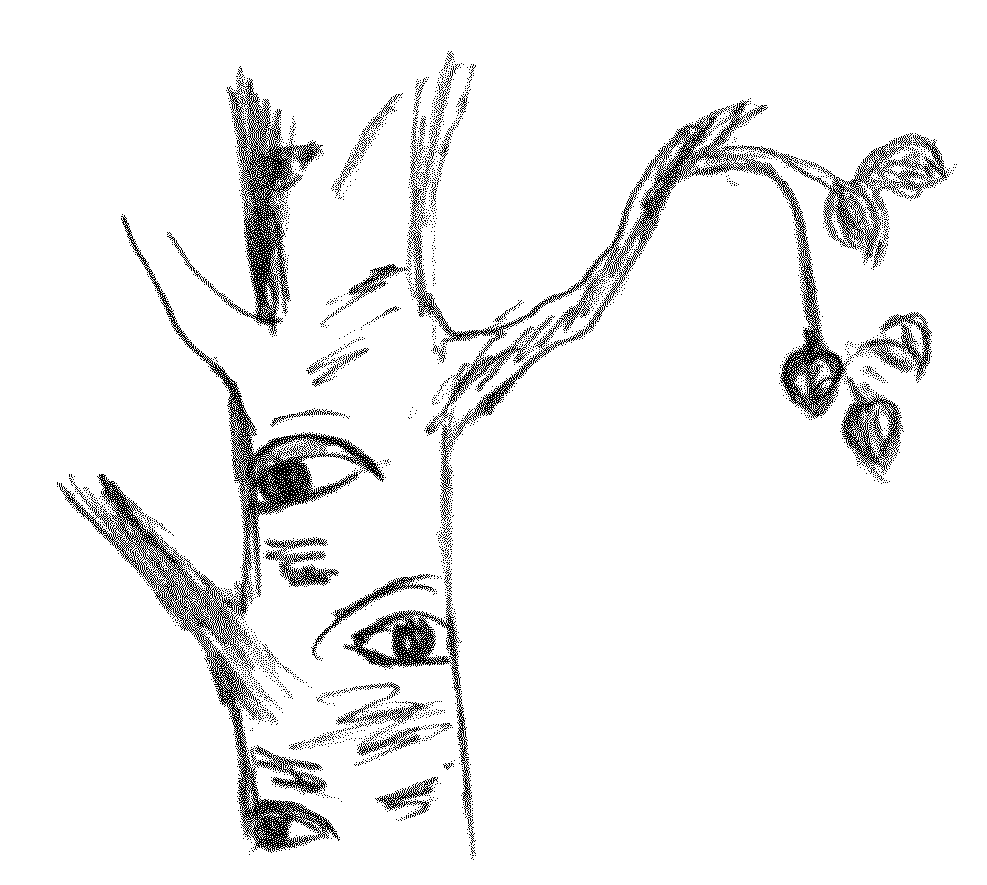
\includegraphics[width=237pt]{birch.png}
\end{center}


\chapter{Processing with RexxXML}

RexxXML is a library for processing XML data. It provides functions for
reading documents, which can be accessed through URLs or Rexx variables, and
for searching and modifying the contents of the documents. It can be used to
transform XML data via XSLT, and to extend XSLT processing.

The preceding chapters introduce Rexx and XML. This chapter gives an overview
of the use of the library.

\section{Initialisation}

Before the library can be used, it needs to be loaded and an
initialisation routine needs to be run. Contrary to some Rexx libraries,
it's not possible to load only the functions you want to use and expect
it to work.

RexxXML can be used both with applications that use Rexx as a macro
language, and with stand-alone Rexx programs. In some cases, the
application will provide the RexxXML API as a built-in component of its
Rexx macro support (it could happen, anyway), but usually the library
must be loaded and initialised explicitly in the Rexx program.
This is done using the built-in function \fn{RxFuncAdd}, which
is discussed in section \ref{sec:rxfuncadd}.

In most cases, the library initialisation should look like this:
\begin{verbatim}
rc = RxFuncAdd('xmlloadfuncs', 'rexxxml', 'xmlloadfuncs')
if rc then do
  say 'Failed to load rexxxml. Reason:' rxFuncErrMsg()
  exit 1
  end
call xmlloadfuncs
\end{verbatim}

\noindent keeping in mind that \fn{RxFuncErrMsg} is a Regina-specific
extension function\footnote{Not a bad idea, though. Other implementations should
adopt it.}. \fn{xmlLoadFuncs} both registers functions with the Rexx
interpreter and initialises the XML library.
If the library is being used with an application which already
uses libxml, it would probably not be good to initialise the library a
second time. This can be disabled by passing an argument (any argument)
to \fn{xmlLoadFuncs}:

\begin{verbatim}
rc = RxFuncAdd('xmlloadfuncs', 'rexxxml', 'xmlloadfuncs')
if rc then do
  say 'Failed to load rexxxml. Reason:' rxFuncErrMsg()
  exit 1
  end
call xmlloadfuncs "don't initialise libxml"
\end{verbatim}

\noindent In cases like this, I recommend that the developer of the application
or the Rexx plug-in consider making the RexxXML functions `built-in'
by calling \fn{rexxXMLInit} and \fn{rexxXMLFini} as appropriate.

\section{Loading documents}

Broadly speaking, there are two approaches to accessing XML data in
wide-spread use: the Simple API for XML, or SAX\index{SAX} approach, which
involves executing a series of user-defined functions as interesting points in
the file are reached, and the Document Object Model or DOM\index{DOM}
approach, which presents the application with a tree representing the document. The
SAX approach is more suited to large data sets where every piece of data needs
to be processed, for instance when a database is dumped to an XML file.
The data is returned to the application as it's read, allowing the
application to use it and get rid of it. On the other hand, the DOM
approach may be more suitable for applications which need to access
only portions of the XML data, since they can deal with the part of
the tree they need and ignore the rest.

libxml, the XML parser underlying RexxXML, provides both SAX- and
DOM-style parsers, however RexxXML provides only a DOM-style
interface. I did this in part to make the interface simpler,
and in part because there's already a Rexx interface to the expat
parser, by Dominik Stein, which provides a SAX-style interface, so people who really
need to serially process a huge data feed can use that instead.

There's one function which converts XML data into a tree, and one
equivalent function for HTML. \fn{xmlParseXML} returns a
document tree corresponding to an XML file, to XML data passed as an
argument, or to XML data passed
as commands in the XML environment. Section \ref{sec:xmlenv}
explains why the latter seemed like a good idea. We can load a file into
a tree in two ways:
\index{xmlParseXML}\begin{verbatim}
doc1 = xmlParseXML('file.xml')
doc2 = xmlParseXML( , charin('file.xml',,100000000))
\end{verbatim}

These functions will fail if the XML data is not well-formed. As used here,
they will expand entity references for entities which were defined in
the internal DTD subset, but they won't load external DTD files,
so entities defined externally will not be expanded.
There's an optional argument which
indicates whether the DTD should be loaded and the document should be
validated.
\index{xmlParseXML}\begin{verbatim}
doc1 = xmlParseXML('file.xml', , 'V') /* validate the file */
doc2 = xmlParseXML('file.xml', , 'D') /* load the DTD, don't validate */
\end{verbatim}

If you modify a document tree and want to turn it back into text, you can
\fn{xmlSaveDoc}\index{xmlSaveDoc}, which converts the document to XML or
HTML as appropriate and saves it to a file or to a Rexx variable.
After processing the data we just loaded, we might write
it out like this:

\index{xmlSaveDoc}\begin{verbatim}
call xmlSaveDoc 'file2.xml', doc1
call lineout 'file2b.xml', xmlSaveDoc( , doc2)
\end{verbatim}

When you're finished with the data, you need to release the tree using
\fn{xmlFreeDoc}\index{xmlFreeDoc}. You can pass it as many trees as you like
in each call.

\begin{verbatim}
call xmlFreeDoc doc1, doc2
\end{verbatim}

If you try to load a file which is not well-formed, or if you validate
and the document is not valid, \fn{xmlParseXML} returns 0. You can get
more information about what went wrong by calling \fn{xmlError}.

\begin{verbatim}
doc = xmlParseXML('file.xml')
if doc = 0 then do
  say 'oops' xmlError()
  return 1
  end
\end{verbatim}

\noindent The error message is intended for human consumption, although
you could conceivably parse some data from it for automatic processing.
If I try to parse this document
\begin{verbatim}
<mydoc>
 <here>is something<wrong>due to improper nesting</here> which is </wrong>
</mydoc>
\end{verbatim}
\noindent I get these errors
\begin{verbatim}
baddoc.xml:2: error: Opening and ending tag mismatch: wrong line 2 and here
 <here>is something<wrong>due to improper nesting</here> which is </wrong>
                                                        ^
baddoc.xml:2: error: Opening and ending tag mismatch: here line 2 and wrong
 <here>is something<wrong>due to improper nesting</here> which is </wrong>
                                                                          ^
\end{verbatim}

\section{Processing document trees}

In the previous section, I said that the parse routines return `a tree'.
The actual return value is a C pointer to a structure which represents
the root node of the tree. This structure has C pointers to other node
structures, and so on. The actual value of the node isn't even remotely useful in
the Rexx language itself.

It's possible to do a lot of things with a tree by passing it to RexxXML
functions. For instance, one can open a document, transform it with
XSLT, and write the result out to a file, or search for a node with
XPath, convert the result to a string and display it. Inevitably, you'll
want to actually do something with the XML data, which means you have to
know how to get the data into a format Rexx can use, and how to
traverse the tree.

Section \ref{sec:treerep} describes the conceptual tree representation
which is the basis of XML processing using XPath. RexxXML follows this
model, but the relationships between nodes are expressed in a slightly
less direct manner than shown there. We'll call the lines between nodes
`links'. The figure in section \ref{sec:treerep} shows links between
every parent node and each of its children. In the trees used by RexxXML,
there are actually links from the parent to its first and last children,
and there are links from each child to its next sibling. The figure
shows these links.

\begin{figure}[htb]\includegraphics{rexxtree}\end{figure}

Suppose we want to process each node in the tree, in the order that the
corresponding elements appear in the document. For each node, we would
first visit all its children in order, then move on to its next sibling.
From the figure, we would first visit the document node, then the comment
node, the `poem' element, the first `stanza' element, the first `line'
element, its text node, the next `line' element, its text node, and so
on through the next two `line' elements, then the second `stanza' element
and its children. In tree-processing circles, this is known as
depth-first traversal.\index{tree!traversing}

To do this in Rexx, we must first convert the node into a stem containing
all the relevant data. I call that process `expanding the node', so the
function which does it is called \fn{xmlExpandNode}\index{xmlExpandNode}. It has two
arguments: the name of the stem, and the node itself. The node stem
is described in section \ref{sec:nodedef}, but I'll mention a few of its tails
here. The most important is probably `type', which says what kind of node
the stem represents. There's also `name', the node's name, `namespaceurl', its
name-space URL, `content',
its text content, and each of the node's attributes, which are
available by name, but with the prefix `a.'. There are also node values
for various parts of the tree: `self' is the node itself; `children' is
its first child; `last' is its last child; `next' is its next sibling;
`prev' is its previous sibling; `attributes' is a list of its attributes;
`parent' is its parent; and `doc' is the root of the tree.

Here's the RexxXML approach to depth-first traversal:

\begin{verbatim}
traverse: procedure
  parse arg node, depth
  if node = 0 then return

  if xmlExpandNode('n.', node) then do
    say copies(' ', depth) || n.name '('n.type')' /* A */
    call traverse n.children, depth+1
    call traverse n.next, depth
    end
  return
\end{verbatim}

\noindent which, when run on the example poem with depth 0 returns

\begin{verbatim}
N.NAME (DOCUMENT_NODE)
 comment (COMMENT_NODE)
 poem (ELEMENT_NODE)
  stanza (ELEMENT_NODE)
   line (ELEMENT_NODE)
    text (TEXT_NODE)
   line (ELEMENT_NODE)
    text (TEXT_NODE)
   line (ELEMENT_NODE)
    text (TEXT_NODE)
   line (ELEMENT_NODE)
    text (TEXT_NODE)
  stanza (ELEMENT_NODE)
   line (ELEMENT_NODE)
    text (TEXT_NODE)
   line (ELEMENT_NODE)
    text (TEXT_NODE)
   line (ELEMENT_NODE)
    text (TEXT_NODE)
\end{verbatim}

This is all well and good, and if all you want is the names of the
elements, everything hopefully seems simple enough. If you want to get at the
data, things can be more complicated. All data is ultimately stored in
text nodes, and can be accessed through the `content' tail of the
expanded nodes. To add the text of the poem to the output from the
previous program, we could add
\begin{verbatim}
    if n.type = 'TEXT_NODE' then
      say copies(' ', depth) n.content
\end{verbatim}
\noindent after the line marked `A' in the last example, and we'd get
output something like
\begin{verbatim}
...
  stanza (ELEMENT_NODE)
   line (ELEMENT_NODE)
    text (TEXT_NODE)
     Once I wondered why the world was so cruel
...
\end{verbatim}

\noindent but it becomes more involved when there are entities involved.
Suppose I replaced `wonder' with the entity reference
`\&thoughtverb;'. This is the sort of thing that will happen more often once
more poets are using XML rather than writing in crayon on scrap paper. 
That fragment becomes
\begin{verbatim}
...
  stanza (ELEMENT_NODE)
   line (ELEMENT_NODE)                A
    text (TEXT_NODE)                  B
     Once I 
    thoughtverb (ENTITY_REF_NODE)     C
     thoughtverb (ENTITY_DECL)        D
      text (TEXT_NODE)                E
       wonder
    text (TEXT_NODE)                  F
     ed why the world was so cruel
...
\end{verbatim}

\noindent Using the letters down the right side for reference, B is the `children'
node of A; C is the `next' node of B; D is the `children' node of C;
E is the `children' node of D; and F is the `next' node of C.
To get the full content of the `line' element, we need to
concatenate all the text nodes that appear as its descendants.
Luckily, the author of RexxXML also uses the library, so there's a
function which does that. We can replace our last modification with

\begin{verbatim}
    if n.type = 'ELEMENT_NODE' & n.name = 'line' then
      say copies(' ', depth) xmlNodeContent(node)
\end{verbatim}

\noindent and get

\begin{verbatim}
...
  stanza (ELEMENT_NODE)
   line (ELEMENT_NODE)
    Once I wondered why the world was so cruel
    text (TEXT_NODE)
    thoughtverb (ENTITY_REF_NODE)
     thoughtverb (ENTITY_DECL)
      text (TEXT_NODE)
    text (TEXT_NODE)
...
\end{verbatim}

There are two ways of getting at attribute values\index{attribute!getting values in Rexx}.
If you know the name
of the attribute in advance, and certain other restrictions don't bother you,
then the value is made available by \fn{xmlExpandNode} in
the tail A.{\it attribute name}\footnote{I wanted to make this @{\it attribute
name} for consistency with XPath, but @ can't be used in symbols with all Rexx
interpreters.}.
For instance, if we want to print the
type of `clause' in the transformed poem on page \pageref{page:otherpoem},
we could add this after the line marked `A' in our tree traversal
routine:

\begin{verbatim}
    if n.type = 'ELEMENT_NODE' & n.name = 'clause' then
      say copies(' ', depth) 'type:' n.a.type
\end{verbatim}

\noindent which would give us

\begin{verbatim}
...
  verse (ELEMENT_NODE)
   lang (ATTRIBUTE_NODE)
    text (TEXT_NODE)
   clause (ELEMENT_NODE)
    type: poetic
...
\end{verbatim}

There are a few restrictions which arise due to rules for Rexx symbols. First,
the tail is the same as the attribute name, but with all letters converted to
upper-case, and without the name-space prefix. Thus if you have two attributes
whose names differ only by case, or more reasonably if you have two attributes
with the same name, but different name-spaces, only one can be accessed this way,
and there's no way of knowing which one. If your attribute name contains
characters which are not allowed in Rexx symbols (-- is a common
example), you need to set a variable to use in the tail:
\begin{verbatim}
  /* attribute names, converted to upper-case */
  fname = 'FIRST-NAME'
  lname = 'LAST-NAME'
  norder = 'NAME-ORDER'
  /* ... */
  if n.a.norder = 'FL' then
    say `Data for' n.a.fname n.a.lname'.'
  else
    say `Data for' n.a.lname n.a.fname'.'
\end{verbatim}

If this method of accessing attributes is inadequate, for instance
because you don't know the names of the attributes in advance, or because
of name-space requirements, you can traverse the `attributes' axis in
the same way as you traverse the `children' axis.  If we take the
original definition of traverse and add this line after the line marked
A:
\begin{verbatim}
    call traverse n.attributes, depth+1
\end{verbatim}

\noindent then we get this output if the original node corresponds to
the transformed poem:
\begin{verbatim}
N.NAME (DOCUMENT_NODE)
 otherpoem (ELEMENT_NODE)
  verse (ELEMENT_NODE)
   clause (ELEMENT_NODE)
    type (ATTRIBUTE_NODE)
     text (TEXT_NODE)
    text (TEXT_NODE)
   clause (ELEMENT_NODE)
    type (ATTRIBUTE_NODE)
     text (TEXT_NODE)
    text (TEXT_NODE)
...
\end{verbatim}

\section{Using and extending XPath}

\label{sec:usexpath}The tree traversal method from the last section can be used as the basis
for a brute-force search algorithm, but searching trees using XPath is
likely to be faster and may be clearer.

A common requirement is to extract data which is embedded in a document.
For instance, you might have a series of specifications, some of which include data
models. The specifications might use a variety of DTDs, depending on the
size and scope of the project they're supporting, but if the data model
is expressed consistently, you can always get at it, provided you can find
its root element, which we'll pretend is called `dataModel'. We could
search the tree like this:

\index{xmlParseXML}\index{xmlExpandNode}\begin{verbatim}
doc = xmlParseXML(filename)
call traverse doc
exit 0

traverse: procedure
  parse arg node
  if node = 0 then return

  if xmlExpandNode('n.', node) then do
    if n.type = ELEMENT_NODE & n.name = 'dataModel' then
      call process node

    call traverse n.children
    call traverse n.next
    end
  return
\end{verbatim}

\noindent For each node in the document, this code converts it to a stem,
checks to see if it's an element called dataModel, and if it is, calls
a procedure called `process'. There's no obvious problem with this,
except that it's likely to waste a lot of time expanding uninteresting
nodes.

Essentially the same thing can be expressed using
XPath:\index{xmlFindNode}\index{xmlNodesetCount}\index{xmlNodesetItem}
\begin{verbatim}
doc = xmlParseXML(filename)
dms = xmlFindNode('//dataModel', doc)
do i = 1 to xmlNodesetCount(dms)
  call process xmlNodesetItem(dms, i)
  end
\end{verbatim}

\noindent \fn{xmlFindNode} returns a node set, from which the individual
nodes can be extracted using \fn{xmlNodesetItem}. Since that's not
obviously better than the tree traversal case, I'll make the search
criteria more complicated. Suppose I was interested only in `table'
elements which appear in the `dataModel', but that there are other
`table' elements which I don't want to deal with, perhaps as content of
`oldDataModel' or something like that. In the tree traversal case, I
might pass a state variable to indicate whether the current node is a
child of `dataModel':

\begin{verbatim}
doc = xmlParseXML(filename)
call traverse doc
exit 0

traverse: procedure
  parse arg node, dadaDataModel
  if node = 0 then return
  if dadaDataModel = '' then dadaDataModel = 0

  if xmlExpandNode('n.', node) then do
    if n.type = ELEMENT_NODE & n.name = 'dataModel' then
      call traverse n.children, 1
    else if dadaDataModel & n.type = ELEMENT_NODE & n.name = 'table'
      then call process node

    call traverse n.children, 0
    call traverse n.next, dadaDataModel
    end
  return
\end{verbatim}

\noindent but the corresponding change in the XPath case is simpler:

\begin{verbatim}
doc = xmlParseXML(filename)
dms = xmlFindNode('//dataModel/table', doc)
do i = 1 to xmlNodesetCount(dms)
  call process xmlNodesetItem(dms, i)
  end
\end{verbatim}

\fn{xmlFindNode} is specifically meant for expressions which return node sets.
\fn{xmlEvalExpression}\index{xmlEvalExpression} evaluates an expression and
returns the result as a string. This can be useful in extracting individual
pieces of information from a document. Suppose we want to extract the invoice
number and customer id from an invoice. We don't need to know the full
structure of the invoice, only that it has an element called `invoice'
which has an attribute called `number' and that it has an element called
`customer' which has an element called `id', and which appears as content of
`invoice'. We could have

\begin{verbatim}
invoiceno = xmlEvalExpression('//invoice/@number', doc)
customer = xmlEvalExpression('//invoice/customer/@id, doc)
\end{verbatim}

\noindent which is clearly simpler than writing tree traversal code,
expanding the node, and dealing with the different kinds of nodes
that appear in the tree.
The expressions in that example both return node sets. \fn{xmlEvalExpression}
returns the string content of the first node in the set.

Variables in the XPath expressions evaluated by \fn{xmlEvalExpression} and
\fn{xmlFindNode} map directly to Rexx variables. For instance,
\begin{verbatim}
name = 'Patrick'
customer = xmlFindNode('//customer[@name=$name]', doc)
\end{verbatim}

\noindent will return a node set containing all the `customer' elements
whose `name' attribute is set to `Patrick'. Note that this is not
true for expressions which are part of XSLT stylesheets, even when
the stylesheet is applied by a Rexx program.

External Rexx functions can be called from XPath expressions
evaluated by \fn{xmlEvalExpression} and
\fn{xmlFindNode} simply by typing their names as if they were
built-in to XPath. The external function will be searched-for according
to the usual rules for whatever Rexx interpreter you use.
Another way to evaluate a function against each node is to evaluate
it as part of the  predicate. 

\begin{verbatim}
customer = xmlFindNode('//dataModel/table[process(.)]/@name', doc)
\end{verbatim}

\noindent This will call an external Rexx function called `process'
once for each table node, passing that node as a node set with one node.
{\it Customer} will be a node set containing any nodes for which
\fn{process} returns a string with length greater than 0.
Scalar values are passed to Rexx functions as strings, but other
types ({e.g.}, node sets) are passed as-is. You need to be aware
of what types your functions expect and what types are being passed.
For instance, this expression passes a node set containing an
attribute to a function

\begin{verbatim}
customer = xmlFindNode('a_function(//dataModel/table[1]/@name)', doc)
\end{verbatim}

\noindent while this one passes a string with the value of that
attribute

\begin{verbatim}
customer = xmlFindNode('a_function(string(//dataModel/table[1]/@name))', doc)
\end{verbatim}

\noindent There's no way from within \fn{a\_function} to tell the two apart.

In the examples in this section, the XPath expressions have been evaluated
with the context node set to the root of the document tree, represented by the
variable {\it doc}. Any other node from the tree would have worked as well,
since I haven't used any relative paths so far. The context node is part of a
larger set of information which makes up the XPath context. libxml has a data
structure corresponding to the XPath context which I'll refer to as a
`context'. RexxXML programs can make limited changes to contexts. In
particular, they can change the context node, and they can register name-space
prefixes for use in node names.

RexxXML provides a context, which I'll call `the default context'\index{default context},
which is normally used by all of its XPath operations. When you call
xmlEvalExpression, the default context's context node is set to the
second argument of the function, and then the first argument is
evaluated. If there is no second argument, the default context is
used with whatever context node it had set before.
I could have written the previous example like this
\begin{verbatim}
invoiceno = xmlEvalExpression('//invoice/@number', doc)
customer = xmlEvalExpression('//invoice/customer/@id')
\end{verbatim}
\noindent without changing the result, although relying on the default
context's pointing at the right spot is probably a bug in the making.

In addition to the default context, contexts can be 
allocated using \fn{xmlNewContext}\index{xmlNewContext}, then passed as the third
argument to \fn{xmlEvalExpression}. This functionality exists
to allow Rexx interfaces to libxml applications to provide
contexts with application-specific functions or variables,
and for use in XSLT extension functions.

\fn{xmlNewContext} takes one or more arguments. The first
one is the context node, while the others are name-space
prefixes in the form ${\it name} = {\it url}$.
Suppose my dataModel elements were part of a name-space.
I need to specify the name-space\index{name-space!in XPath} when searching.
I might have:
\begin{verbatim}
ctxt = xmlNewContext(doc, 'dm=http://www.interlog.com/~ptjm/dataModel')
tables = xmlFindNode('//dm:table',,ctxt)
\end{verbatim}

The context node can be changed, and new name-space prefixes added,
using \fn{xmlSetContext}\index{xmlSetContext}. Its first argument is the context, the
second is the new context node, and any others are name-space
prefixes. If the context argument is left blank, the function modifies
the default context.\index{default context}:

\begin{verbatim}
ctxt = xmlSetContext(, doc, 'dm=http://www.interlog.com/~ptjm/dataModel')
tables = xmlFindNode('//dm:table')
\end{verbatim}

\noindent My advice is to use \fn{xmlSetContext} if you need to set a
name-space prefix in the default context, but otherwise ignore it.

All of the examples to this point pass an XPath expression as a string.
This string will be compiled into a form which can be evaluated quickly,
and then that form is evaluated. It's also possible to compile the string once,
and evaluate the compiled form repeatedly.
This may result in some time savings, especially if the expression is
complicated. Note that variables are evaluated at the time the expression
is evaluated, not at the time it is compiled. This code saves
each `table' element which is a child of the node in the variable {\it dmnode}.
\index{xmlCompileExpression}\index{xmlEvalExpression}
\begin{verbatim}
ce = xmlCompileExpression('table[number($i)]')
call xmlSetContext , dmnode

do i = 1
  tabs.i = xmlFindNode(ce)
  if tabs.i = 0 then leave
  end
tabs.0 = i-1
\end{verbatim}

\noindent Note that each {\it tabs.i} is set to a node set with a single
node in it. In this case, it would probably be more efficient to return a single node
set with all the table nodes in it, then enumerate it using
\fn{xmlNodeSetItem}, but the point is that a compiled expression is equivalent
to but slightly faster than the expression as a string. One of my test
scripts using compiled expressions runs 10\% faster than an equivalent script
using strings.

In addition to the function interface to XPath, there's an environment
called XPath\index{XPath!environment}\index{environments} which evaluates expressions
against the default context and assigns their results to the variable {\it
RC}. This environment exists only because I thought an XSLT environment
would be a good idea, then I rationalised that an XML environment might
be useful in some circumstances, and at that point I suppose I was a bit
environment-happy. Environments are normally evaluated for side-effects,
but XPath expressions are evaluated for their return values, so it's an
odd match. If you do find it helpful, be sure to set the trace level to
o.

\begin{verbatim}
trace o
address XPath
'//dataModel/table'
dms = rc
do i = 1 to xmlNodesetCount(dms)
  call process xmlNodesetItem(dms, i)
  end
\end{verbatim}

\section{Using and extending XSLT}

XSLT can be used to provide transformations as an adjunct to RexxXML
processing, and Rexx can be used to extend XSLT. If you have a program
which processes some set of XML tags, it can be extended to support
any equivalent set of tags by writing a stylesheet to perform the
conversion.

Suppose the function `process' does something useful with some XML data
whose root element is `data'. Suppose further that there are three
data feeds, one of which delivers these `data' documents, another
of which delivers an equivalent-but-different structure whose root
element is `Data', and the last of which delivers a third set of
equivalent tags whose root is `DATA'. We can pass all three feeds
to `process' provided we do a little transformation first:
\index{xmlApplyStylesheet}\index{xmlParseXSLT}\begin{verbatim}
doc = xmlParseXML(datafile)
tx = xmlParseXSLT('Datatodata.xsl')

if \ xmlNodesetCount(xmlFindNode('/data', doc)) then do
  doc2 = xmlApplyStylesheet(tx, doc)
  call xmlFreeDoc doc
  doc = doc2
  end

call process doc
call xmlFreeStylesheet tx
call xmlFreeDoc doc
\end{verbatim}

As with XML, XSLT data can be loaded from a file,
read from a Rexx expression,
or embedded as an environment (using address XSLT).
\fn{xmlApplyStylesheet}
takes as arguments either a parsed stylesheet and an XML document
tree, or URLs for a stylesheet file and an XML document, or
some combination of the two. The third and fourth arguments are
used to distinguish between these options.

\begin{verbatim}
doc2 = xmlApplyStylesheet('Datatodata.xsl', datafile, 'url', 'url')
\end{verbatim}

Any arguments after
the third and fourth arguments are pairs of parameter names
and parameter values expressed as XPath expressions.\index{arguments!XSLT stylesheet}
These values take the place of the top-level xsl:param entries in the
stylesheet.
For whatever reason, it's traditional for XSLT
parameters to be passed as XPath expressions. This means a number
will be treated as a number, \fn{true} will be treated as a Boolean
function, a string in quotes will be treated as a string, and
almost everything else will result in an error, since there's no
XPath context at parse time. This leads to problems in the common case
where the parameter is meant to be a string. To make things simpler,
RexxXML tries to treat parameter values intelligently. Things that look
like numbers are treated as numbers, and things that look like strings
are treated as strings. The rules are laid out in section
\ref{sec:xmlapplystylesheet}, but hopefully this example will give you a
feel for them (the commas at the ends of the lines are continuations~--
I said they could be confusing).

\begin{verbatim}
res = xmlApplyStylesheet(ss, doc,,,                ,
          'name', 'Patrick McPhee',  /* string */  ,
          'height', 175,             /* number */  ,
          'weight', 'true()',        /* Boolean */ ,
          'shiraz', "'92'")          /* string */
\end{verbatim}


I mentioned in section \ref{sec:extensions} that XSLT processors are
allowed to provide extended functionality, provided the stylesheet has
to explicitly request it by declaring a name-space.
RexxXML provides extension elements which allow Rexx scripts to be
embedded in XSLT stylesheets, controlled by the name-space
urn://rexxxml\slash xslt. In this discussion,
I'll use the name-space prefix `rexx' to distinguish them.

Keep in mind that there are extensions and there are extensions.
If you find it difficult to do something in XSLT, it's tempting
to work around it by writing code in a different language. The more
extensions you use, the less portable your stylesheets become, which
sometimes can be an issue. In particular, if you want to use stylesheets
to transparently modify documents returned by an HTTP server, you need
to restrict yourself to extensions which are supported by your target
audience. This is likely to include EXSLT and probably something based
on ECMAscript, but unfortunately not Rexx. If you control the execution
environment, then portability might be less important, and hopefully
these extensions will free up some spare time so you can write that
novel you've been meaning to get to.

rexx:rexx\index{rexx:rexx} contains a Rexx script which is invoked each
time the stylesheet is parsed. This script can't generate output,
but it can do things like make database connections, load function
libraries, and delete output files from previous runs.

When Rexx scripts are defined in a stylesheet, they're treated much
like external functions.  They have no access to functions or variables
defined in the script that called \fn{xmlApplyStylesheet}, for instance,
nor do they have access to global variables set by other scripts
within the same stylesheet. You can get around this last limitation
by setting environment variables using \fn{value}\index{value!environment variables}.

If we want to use RexxXML in conjunction with Rexx/SQL\index{Rexx/SQL},
we'd want to make a database connection at the start of processing:

\begin{verbatim}
<xsl:stylesheet version="1.0" xmlns:xsl="http://www.w3.org/1999/XSL/Transform"
  xmlns:rexx="urn://rexxxml/xslt"
  extension-element-prefixes='rexx'>
 <xsl:include href='dbtemplates.xsl'/>

 <rexx:rexx><[CDATA[/* connect to the database */
     Call RxFuncAdd 'SQLLoadFuncs', 'rexxsql', 'SQLLoadFuncs'
     Call SQLLoadFuncs
     if  SQLConnect('c1', 'scott', 'tiger') < 0 then do
        say 'database connection failed'
        say 'I can''t return an error, though'
        say 'McPhee should do something about this'
        end
     else
        call value 'DB_CONNECTION', 'c1', 'ENVIRONMENT'
 ]]></rexx:rexx>
</xsl:stylesheet>
\end{verbatim}

\noindent This script is in a CDATA section so I don't have to worry
about things like \& and $\langle$ not being allowed in XML data.
At present there's no way to signal an error in a Rexx script.\index{to
do!revisit errors in rexx:rexx et al} I get around that in this case by
setting the environment variable indicating the connection id
only when it's been made successfully. There are presumably templates in
dbtemplates.xsl which will retrieve that environment variable and behave
appropriately if it isn't set.

A significant problem with using rexx:rexx to perform initialisation is
that there's no corresponding element which gets executed when the
stylesheet is deallocated. One way to resolve this is to perform
initialisation and clean-up in the program that calls
\fn{xmlApplyStylesheet}. This gives you control over when these
operations are performed, but may make the stylesheet harder to
re-use. You could also wait until some future date when I've resolved
the issue\index{to do!update on fini processing}. Perhaps the best thing
is to invoke the initialisation and termination processing as part of
a template which matches the root element, using rexx:template, which
by a remarkable coincidence is the subject of the next paragraph or so.

rexx:template\index{rexx:template} can appear anywhere template content
is allowed. That is, anywhere xsl:value-of is permitted. Its content
is a template which is expanded, then processed as a Rexx script. The
script can be evaluated for side-effects, or it can return data for
inclusion in the result tree. It has access to XPath context of the
surrounding template, and any attributes of the template element
are treated as variables, which are initialised
before the script is invoked.

What that all means is that rexx:template contains a script which can
incorporate data from the target document by using \fn{xmlEvalExpression},
interpolating data expanded from xsl:value-of and other XSLT elements, or
using pre-initialised variables. Assuming it's not a problem to open a
new database connection each time I process a new document, I could
rewrite my rexx:rexx example like this:

\begin{verbatim}
<xsl:stylesheet version="1.0" xmlns:xsl="http://www.w3.org/1999/XSL/Transform"
  xmlns:rexx="urn://rexxxml/xslt"
  extension-element-prefixes='rexx'>
 <xsl:import href='dbtemplates.xsl'/>

 <xsl:template match="/">

   <rexx:template><[CDATA[/* connect to the database */
       Call RxFuncAdd 'SQLLoadFuncs', 'rexxsql', 'SQLLoadFuncs'
       Call SQLLoadFuncs
       if  SQLConnect('c1', 'scott', 'tiger') < 0 then do
         say 'database connection failed'
         end
       else
          call value 'DB_CONNECTION', 'c1', 'ENVIRONMENT'
   ]]></rexx:rexx>

   <!-- whatever was defined for / in dbtemplates.xsl gets used here -->
   <xsl:apply-imports/>

   <rexx:template><[CDATA[/* release the database */
       c1 = value('DB_CONNECTION',,'ENVIRONMENT')
       if c1 \= '' then
         call SQLDisconnect c1
   ]]></rexx:rexx>
 </xsl:template>
</xsl:stylesheet>
\end{verbatim}

\noindent Since I now have access to the target document, I can extract
information from it, say the user name and password. I recommend doing
it this way:

\begin{verbatim}
   <rexx:template user='{/data/@refusername}'
                  password='{/data/@refpassword}'
                  all-strings='yes'>
     <[CDATA[/* connect to the database */
       Call RxFuncAdd 'SQLLoadFuncs', 'rexxsql', 'SQLLoadFuncs'
       Call SQLLoadFuncs
       if  SQLConnect('c1', user, password) < 0 then do
         say 'database connection failed'
         end
       else
          call value 'DB_CONNECTION', 'c1', 'ENVIRONMENT'
   ]]></rexx:rexx>
\end{verbatim}

There are three attributes on this rexx:template element. One of them,
`all-strings', is defined by the library, while the other two are the names of
Rexx variables which will be set when the script is invoked. The variable
values can be attribute value templates\index{attribute value template} (see
section \ref{sec:templatecontent}), so the data can be taken, as in this case, 
from the target document. If `all-strings' is set to true, then
the variable values are treated as strings. Otherwise, scalar values
are passed as strings, but node sets and document tree fragments are
passed as nodes.

rexx:template inserts data into the result tree by returning it.
In this case, we look up a value in the database and return it if
found, or the key if it wasn't found:

\begin{verbatim}
   <rexx:template name='{.}' all-strings='yes'>
     <[CDATA[/* look up the full name */
       if SQLCommand('c1', 'select fullname from names where ncode=:name',  ,
             ':name', name) < 0 then do
         say 'lookup failed'
         return name
         end
       else if c1.fullname.0 > 0 then return c1.fullname.1
       else return name
   ]]></rexx:rexx>
\end{verbatim}

\noindent The return value can be a string value, a node set, or a
document tree. The latter two are discussed further in section \ref{sec:doctree}
and full documentation for rexx:template is in section \ref{sec:rexx:template}.

In addition to any variables set through attributes, there are three pre-set
variables available to rexx:template scripts. {\it
xmlContext}\index{xmlContext} holds the XPath context for use in evaluating
XPath expressions, while {\it xmlResultTree}\index{xmlResultTree} is the current
result tree, which you can search, write to a file, or modify directly, and
{\it xmlResultNode}\index{xmlResultNode} is the node after which the return
value of the script will be inserted. If you add new nodes directly in the
script, you should set {\it xmlResultNode} to the last node you add. You can
go as far as freeing the current result tree and creating a new one. If you
do, you should set both {\it xmlResultTree} and {\it xmlResultNode} to the
root of the new tree. Any time you remove nodes from the result tree, be
careful that the template which called your
script wasn't in the middle of generating or updating those nodes.

This example searches the target document (through {\it xmlContext})
and the result tree for an `author' node, assumes that it finds
them, and ensures that the text content is the same.
\index{xmlFindNode}\index{xmlRemoveContent}\index{xmlAddText}\begin{verbatim}
<rexx:template>
inaut = xmlFindNode('//author',,xmlContext)
outaut = xmlFindNode('//author',xmlResultTree)

if xmlNodeContent(inaut) != xmlNodeContent(outaut) then do
  call xmlRemoveContent outaut
  call xmlAddText outaut, xmlNodeContent(inaut)
  end
</rexx:template>
\end{verbatim}

The last extension element defined by RexxXML is rexx:function\index{rexx:function}. It
defines a function which can be called from any XPath expression
in the stylesheet. Any function you define this way has to have a
name-space associated with it. You should associate it with a URL
based on some network address with which you have an association.
It's common to base the URL on a web-site address, which is long and
inconvenient, but likely to avoid the sort of conflict name-spaces are
supposed to avoid.

rexx:function has three attributes: `name', the name of the
function, including the name-space prefix; `return-type', the
type to return to the XPath expression; and `all-strings', which
has the same meaning as it did for rexx:template, except that it
applies to function arguments rather than preset variables. `return-type'
is important if you need the function to work in certain contexts.
For example, if the function is for use in a predicate, it should
have a return type of `Boolean'. 
\begin{verbatim}
<xsl:stylesheet version="1.0" xmlns:xsl="http://www.w3.org/1999/XSL/Transform"
  xmlns:rexx="urn://rexxxml/xslt"
  xmlns:prd="http://www.interlog.com/ptjm/predicate-example"
  extension-element-prefixes='rexx'>
 <rexx:function name="prd:random-selection" return-type='Boolean'>
   if random() > 500 then return 'true'
   else return 'false'
 </rexx:function>

 <xsl:template match='node()[prd:random-selection()]'>
    <xsl:copy>
       <xsl:apply-templates/>
    </xsl:copy>
 </xsl:template>
</xsl:stylesheet>
\end{verbatim}

Functions can return node sets (using the `return-type' value `node set'). To
create a node set, use \fn{xmlNodesetAdd}\index{xmlNodesetAdd}. It takes two or
more arguments, the node set and nodes to add to it. If the node set is left blank,
a new node set is created.
\begin{verbatim}
return xmlNodesetAdd(, node1, node2, node3, node4)
\end{verbatim}
\noindent or
\begin{verbatim}
ns = ''

do while someTest()
  node = someNode()
  ns = xmlNodesetAdd(ns, node)
  end
return ns
\end{verbatim}


The automatic invocation of external Rexx functions available in
\fn{xmlEvalExpression} doesn't work in stylesheets. I originally
implemented functions for registering external functions, and an
extension function for executing them without registering them,
but then I decided that this didn't add anything, so I removed it.
If you want to call an external function, call it from a function
defined by rexx:function.
\begin{verbatim}
 <rexx:function name="prd:external-call">
   parse arg a,b,c
   return 'my-function'(a, b, c)
 </rexx:function>
\end{verbatim}

\section{Building document trees}

\label{sec:doctree}To this point, almost everything I've mentioned
had to do with extracting data from an XML document. Those documents
have to come from somewhere, and I suppose it's natural to want an
API for generating them. I feel bound to point out that XML is a
text-based data format, and the easiest way to generate it is probably
to concatenate together a bunch of strings.

\begin{verbatim}
data = '<data>'
do i = 1 to chunks.0
   data = data || '<chunk>' || chunk.i || '</chunk>'
   end
data = data || '</data>'
doc = xmlParseXML(,data) /* if you need to search the data */
\end{verbatim}

\noindent There will be problems with this approach if the data is not in the
character set of the target document, or if it includes the characters
\verb+<+ or \verb+&+, but this can be resolved without adopting a
specialised API.

There are two common cases where an API for generating XML data is
needed. One is to make modifications to an existing XML document,
and the other is when adding data to an XSLT result tree. In the former
case, we must either modify the tree generated by \fn{xmlParseXML} or
modify the original document directly, which would require writing an
XML parser in Rexx. In the latter case we have no choice but to work
directly with the tree representation.

Modifying a document requires creating the appropriate types of nodes
and inserting them in the appropriate location in the tree. RexxXML
provides a number of routines to assist in this process.
To create the document tree from the last example, we might do this

\index{xmlNewDoc}\index{xmlAddElement}\begin{verbatim}
doc = xmlNewDoc()
node = xmlAddElement(doc, 'data')

do i = 1 to chunks.0
   call xmlAddElement node, 'chunk', chunks.i
   end
\end{verbatim}

\noindent which on reflection seems shorter and simpler. XML must be the
anti-Rexx. In addition to \fn{xmlAddElement}\index{xmlAddElement}, there are
\fn{xmlAddAttribute}\index{xmlAddAttribute}, \fn{xmlAddText}\index{xmlAddText}, \fn{xmlAddPI}\index{xmlAddPI}, and
\fn{xmlAddComment}\index{xmlAddComment}, each of which creates a node of the appropriate type
and inserts it somewhere relative to the node given in the first
argument, {\it node}. The default behaviour\footnote{except for
\fn{xmlAddAttribute}} is to insert the new node at the end of
{\it node}'s children, but through an optional argument, the routines
can be directed to insert the new node either before, after, or in place
of {\it node}.

Suppose you have a few hundred HTML files which load images from a
subdirectory called `img', and suppose your corporation has introduced a
new corporate transparency standard which requires that HTML images be
loaded from a directory called `image'. I'm making this up, but it's
exactly the sort of thing that happens all the time. You have a few
thousand tags like this
\begin{verbatim}
<img width="8%" src="img/tree.png">
\end{verbatim}
\noindent which need to end up looking like this
\begin{verbatim}
<img width="8%" src="image/tree.png">
\end{verbatim}

We want to find all the img tags which have this problem, then replace
the src attribute. We could do it like this:

\index{xmlParseHTML}\index{xmlAddAttribute}\begin{verbatim}
doc = xmlParseHTML(doc.i)
imgs = xmlFindNode('//img[substring(@src, 1, 4) = "img/"], doc)
do i = 1 to xmlNodesetCount(imgs)
   node = xmlNodesetItem(imgs, i)
   txt = xmlEvalExpression('@src', node)
   rc = xmlAddAttribute(node, 'src', 'image' || substr(txt, 4))
   if rc = 0 then panic_and_die()
   end
call xmlSaveDoc 'newdir/'doc.i, doc
\end{verbatim}

If the value being replaced were not an attribute value, we'd
have to alter or replace the text node directly. Since we can also do this
with an attribute value, I'll demonstrate two other approaches to the
same problem. I want to change a child of the attribute value, so I need
to use an XPath expression which returns all the relevant src attributes.
After that, I can delete the current content and add new text

\index{xmlRemoveContent}\index{xmlAddText}\begin{verbatim}
imgs = xmlFindNode('//img/@src[substring(., 1, 4) = "img/"], doc)
do i = 1 to xmlNodesetCount(imgs)
   node = xmlNodesetItem(imgs, i)
   txt = xmlEvalExpression('.', node)
   call xmlRemoveContent node
   rc = xmlAddText(node, 'image' || substr(txt, 4))
   if rc = 0 then panic_and_die()
   end
\end{verbatim}

\noindent We can also manipulate the text nodes directly. This time I
use the optional argument to \fn{xmlAddText} to say that {\it node}
is a text node and I want to replace its content with the new text

\begin{verbatim}
imgs = xmlFindNode('//img/@src/text()[substring(., 1, 4) = "img/"], doc)
do i = 1 to xmlNodesetCount(imgs)
   node = xmlNodesetItem(imgs, i)
   txt = xmlEvalExpression('.', node)
   rc = xmlAddText(node, 'image' || substr(txt, 4), 'replace')
   if rc \= node then panic_and_die()
   end
\end{verbatim}

This last approach can be useful for a large set of text processing
applications. Suppose you want to highlight the word `infrastructure'
throughout a document. We could use XPath to find the nodes, then
\fn{xmlAddText} and \fn{xmlAddElement} to replace the current text node
with the appropriate nodes.

\index{translate}\begin{verbatim}
inf = 'INFRASTRUCTURE'
linf = length(inf)
expr = "//text()[contains(., 'infrastructure') or contains(., 'Infrastructure')]"
nds = xmlFindNode(expr, doc)
do i = 1 to xmlNodesetCount(nds)
   node = xmlNodesetItem(nds, i)
   call xmlExpandNode 'nd', node
   text = nd.content
   txt = translate(text)
   pos = pos(inf, txt)
   rep = 'Replace'

   do while pos > 0
     if pos > 1 then do
       node = xmlAddText(node, substr(text, 1, pos-1), rep)
       rep = 'After'
       end
     node = xmlAddElement(node, 'em', substr(text, pos, linf), rep)
     rep = 'After'
     txt = substr(txt, pos+linf)
     text = substr(text, pos+linf)
     pos = pos(inf, txt)
     end

   if length(text) > 0 then
     node = xmlAddText(node, text, rep)
   end
\end{verbatim}

\noindent After the original text node is replaced using `Replace',
subsequent nodes are added as its siblings using `After'. If the
constant setting of {\it rep} proved to be a bottleneck, the first-node
processing could be moved out of the loop, at the expense of duplicating
the processing logic.

Another common processing task is inserting boilerplate. For some
situations, the functions I've mentioned so far are adequate.
\index{xmlAddComment}\begin{verbatim}
doc = xmlParseXML(doc.i)
call xmlAddComment doc, ' Copyright 2003, Corporation X'x2c('0a')  ||,
                        '     All rights reserved'x2c('0a')        ||,
                        '     Why are you still reading this? '
call xmlSaveDoc 'newdir/'doc.i, doc
\end{verbatim}

Suppose we wanted to re-use the disclaimer section from an existing
document. \fn{xmlCopyNode}\index{xmlCopyNode} creates a freelance node which can be added
to another document ({\it nd.children} is the document element):
\begin{verbatim}
disc = xmlFindNode('//disclaimer', doc)
if xmlNodesetCount(disc) > 0 then do
  mydisc = xmlCopyNode(xmlNodesetItem(disc, 1)
  call xmlExpandNode 'nd', doc2
  call xmlAddNode nd.children, mydisc /* adds disclaimer at the end */
  end
\end{verbatim}

\noindent This technique can be used to create any type of node, so for
instance there's no API for creating a DTD, but one can add an entity
declaration by creating a document with the appropriate
entity declaration in its internal subset, parsing it, locating
the entity declaration (using \fn{xmlExpandNode} since XPath doesn't
support DTDs at all), copying the declaration node, then adding the
copy to the target document.

\index{XML!environment}\begin{verbatim}
address XML
'<!DOCTYPE data [<!ENTITY rice "ordinary, boring rice">]> <data/>'
edoc = xmlParseXML()
call xmlExpandNode 'enode', edoc
intss = enode.intsubset
rcc = xmlExpandNode('enode', intss)

do until \rcc | enode.type = 'ENTITY_DECL'
  rcc = xmlExpandNode('enode', enode.children)
  end

if rcc then entdecl = enode.self

tdoc = xmlParseXML('needrice.xml')
call xmlExpandNode 'tnode', tdoc

if tnode.intSubset \= 0 then
   call xmlAddNode tnode.intSubset, entdecl
else if tnode.extSubset \= 0 then
   call xmlAddNode tnode.extSubset, intss, 'before'
else if tnode.children \= 0 then
   call xmlAddNode tnode.children, intss, 'before'
else
   call xmlAddNode tnode.self, intss

call xmlSaveDoc 'hasrice.xml', tdoc
call xmlFreeDoc tdoc
\end{verbatim}

Note that I didn't free {\it edoc} at the end of all that. This is
because \fn{xmlCopyNode}\index{xmlCopyNode} doesn't support copying
DTD nodes, so I've linked either the internal subset or the entity
declaration from {\it edoc} directly into {\it tdoc}. You might almost
describe this operation as a miserable kludge, but DTDs aren't a big
thing in XML processing, so you shouldn't have to do this too often.

Another, possibly safer, approach to the same problem is to create a
new document with the appropriate internal subset, and graft a copy
of the real document onto it. As sometimes happens, the safe, reliable
way is probably clearer and involves less typing.

\begin{verbatim}
tdoc = xmlParseXML('needrice.xml')

/* build a file with the appropriate entity declaration and an empty
 * document element */
root = xmlEvalExpression('name(/*)', tdoc)
address xml
'<!DOCTYPE' root '[<!ENTITY rice "ordinary, boring rice">]><'root'/>'
edoc = xmlParseXML()

/* add a copy of the source's document element in place of the
 * document element of the new document (which has been
 * carefully constructed so that the document element is the
 * last node  */

call xmlExpandNode 'enode', edoc
call xmlExpandNode 'tnode', tdoc
call xmlAddNode enode.last, xmlCopyNode(tnode.children), 'replace'

call xmlSaveDoc 'hasrice.xml', edoc
call xmlFreeDoc tdoc, edoc
\end{verbatim}

\section{Schema validation}

We typically want to do two things with schemas: validate documents
using them, and programmatically figure out what they say. Currently,
document validation is the only feature provided by RexxXML, which
might be inconvenient, but has the advantage that this section will be
quite short.

There are only four functions associated with schemas: \fn{xmlParseSchema},
\fn{xmlValidateDoc}, \fn{xmlFreeSchema}, and \fn{xmlDumpSchema}\index{xmlParseSchema}\index{xmlValidateDoc}\index{xmlFreeSchema}\index{xmlDumpSchema}.
As with XML and XSLT, schemas can be read from a file, a Rexx variable,
or the XSD environment. As with applying stylesheets, you have the option
of parsing the schema and target document, then passing the tree
representations to \fn{xmlValidateDoc}, or you can pass file names
instead.

Instead of numeric return codes, \fn{xmlValidateDoc} returns the string
`OK' if the document validated correctly, and one of a large set of
strings if there was a problem. I expect you to ignore all the error
codes and use \fn{xmlError} to find out what's going on. Here's
the typical usage:

\begin{verbatim}
xsd = xmlParseStylesheet('mytypes.xsd')
do i = 1 to files.0
  if xmlValidateDoc(xsd, files.i) \= OK then do
     say xmlError()
     drop files.i
     end
  end     
call xmlFreeStylesheet xsd
\end{verbatim}

The other usage scenario has a document tree being built up in the Rexx
program, then passed to \fn{xmlValidateDoc}. In a future release, I
would like to provide routines for reporting and more localised
validation, but this functionality is not immediately available
from libxml, and I've decided to hold it back in favour of actually
releasing the library while XML is still in widespread use.

\section{Examples}

The distribution includes a handful of example scripts, which generally
perform simple tests of the library.
This section describes a few of them and tries to give a sense of how
they were developed.


\subsection{Dump File}

\label{sec:dumpfile}This is actually based on the first program ever written for RexxXML. Of
course, in those days, it was called `xml01.rex' and the library itself was
called `xxrexx', but it still has a special place in my heart. Today, the
program consists of two scripts, `dumpfile.rex' and
`treewalk.rex'.\index{treewalk.rex}\index{dumpfile.rex}

The point of writing xml01 was to get familiar with the library and
change things that seemed cumbersome or stupid. My premise was that, whatever
other features the library had, if I could write a Rexx program which visited
every node in the tree representation of a document, the library could be used
to solve problems through brute force traversal of the document, and I could
dismiss any user problems as design limitations. As it turns out, the
treewalk function can be a useful debugging tool.

`dumpfile' opens an XML file specified by the user, then passes the document
tree to `treewalk', which reports the contents of the tree. It's short,
and I haven't really given a complete example of a Rexx program yet,
so I'll comment on every line, in order. The program starts with
a comment.
\begin{verbatim}
/* Load XML data from a URL, then dump its structure using treewalk.rex
 *
 * $Header : /usr/home/ptjm/rexx/rexxxml/trip/RCS/dumpfile.rex 1.7 2003/10/16 17:20:17 ptjm Exp $
 */
\end{verbatim}

\noindent As I mentioned before, some interpreters require a comment at the
start of the program. It's not uncommon to see programs start with an
empty comment (\verb+/* */+) on such systems, but it's better to have a short
description of the file. The \$Header{}: \dots \$ that you'll see in a lot
of my source files is version control information which is filled in by
RCS, the revision control system. It's a really good idea to get and use
revision control software for all your programs. There's nothing more
frustrating than having an algorithm working, then making a few
uncontrolled changes and never getting it working again. It's even more
frustrating than watching both the Cubs and the Red Sox blow three-run
leads with one out in the eighth because their managers don't trust their
bullpens. If you get into the habit of checking files in to a revision
control system whenever you're about to tweak something that's already
working, you won't have to face this frustration.

Getting back to `dumpfile', the next few lines get the URI for the
file we'll be dumping from a command-line argument, or complain
and exit if no argument was given.

\begin{verbatim}
parse arg uri .

if uri = '' then do
  say 'usage: dumpfile <filename>'
  exit 1
  end
\end{verbatim}

\noindent I do that before loading the library as a micro-optimisation.
The next few lines could be repeated in every program that uses
RexxXML. They load the library, then call \fn{xmlLoadFuncs}.

\begin{verbatim}
rcc = rxfuncadd('XMLLoadFuncs', 'rexxxml', 'xmlloadfuncs')

if rcc then do
  say 'error' rcc 'loading RexxXML'
  say rxfuncerrmsg()
  exit 1
  end

call xmlloadfuncs
\end{verbatim}

There are only three lines of true program logic. First I load the
specified file, and report an error if the load fails,

\begin{verbatim}
nd = xmlparsexml( uri)

if nd = 0 then say 'bad' uri xmlError()
\end{verbatim}

\noindent and then I call `treewalk'. The quotes around the function
name are to prevent the Rexx interpreter from converting the name to
upper-case. Since treewalk is an external function, the name specified
in the program must match the name of the file containing the program,
and Unix file systems are case-sensitive.

\begin{verbatim}
call 'treewalk' nd, 0, uri
\end{verbatim}

Treewalk is the routine that actually traverses the document tree.
It takes three arguments~-- a node, an indentation level, and
a title to display at the start of the dump. It calls \fn{xmlExpandNode}
to assign the node to a stem, then displays the values of each tail.
Finally, it calls itself recursively for each child node in the tree.

Treewalk starts with another comment, then it parses out its arguments.
This parse statement is a bit different from the one in dumpfile.
\begin{verbatim}
parse arg tree, indent, title
\end{verbatim}

\noindent Because treewalk is invoked as a function, it can parse out
more than one argument, separated by commas. Normal rexx commands
never have more than one argument. The arguments in this case are
the XML tree, the indent level (in the call above, 0), and some text
to print as a title (the name of the file).

The function next sets up a stem called hex. First it makes 0 the
default value for the stem, then it sets each of the tails set
by \fn{xmlExpandNode} which correspond to nodes of the tree to 1.
\begin{verbatim}
hex. = 0
hex.intsubset = 1
hex.extsubset = 1
hex.self = 1
...
\end{verbatim}

\noindent These tails contain binary data and will be printed in
hexadecimal notation. Next the variable {\it tails} is set to the names of all
the tails set by \fn{xmlExpandNode}. In the original version of the routine, the
tails were determined dynamically. This can be done in IBM's
Object Rexx using the syntax `do $x$ over $y.$', and with Regina or
Rexx/IMC using Regutil's \fn{regStemDoOver}, but there's no portable
way to retrieve tails dynamically. Apart from that, putting
the names of the tails in a list ensures that they are presented in
a consistent order for all nodes. The commas here are line continuation
characters.

\begin{verbatim}
tails = 'TYPE NAME SELF PREV NEXT CHILDREN LAST PARENT NAMESPACEPREFIX' ,
        'NAMESPACEURL URL EXTERNALID SYSTEMID CONTENT ENCODING VERSION' ,
        'INTSUBSET EXTSUBSET COMPRESSION STANDALONE ATYPE ETYPE'        ,
        'MANDATORY ATTRIBUTES A'
\end{verbatim}

All of that is done once for each call to the external procedure.
The of treewalk's work is done by recursively calling an internal procedure
of the same name, and the last thing the external procedure does is
to call this internal procedure, passing the same three arguments.

\begin{verbatim}
call treewalk tree, indent, title
return
\end{verbatim}

The internal routine starts by parsing out the arguments, then
returning immediately if the current node {\it cur} is 0, meaning
we've reached the end of the list of nodes. This will happen,
for instance, if there are no attributes for an element, or
if the current node has no next sibling.
After printing the title, {\it indent} is set to the
appropriate number of spaces to get the current indentation level.

\begin{verbatim}
treewalk: procedure expose hex. tails

  parse arg cur, ind, title

  if cur = 0 then return
  if ind > 0 then say ''
  say title

  indent = copies('  ', ind)
\end{verbatim}

The heart of the routine assigns each of the names in {\it tail} to
{\it i}, tests to see if the tail was set for the node, and if so,
displays it. \fn{Symbol} returns `LIT' if its argument is a literal
symbol, and `VAR' if it's been assigned a value. In this example,
it's used both to determine whether a particular tail is set
and to determine whether there are any attributes. {\it Tail}
is effectively a constant list of all possible tails which
could be part of an expanded node. Not all values will be
set for all nodes, and reporting unset nodes can only
clutter up the screen and cause confusion, so we skip
unset values. By contrast, {\it sft.a} is a list of all the attributes
that are actually set, and we can loop through them without testing,
so long as {\it sft.a} has a value.

{\it Hex.i} evaluates to true for any tail that contains a node. These
values are displayed in hexadecimal notation with a trailing `x',
unless their actual value is 0, in which case they're displayed as
themselves. Other values are displayed with guillemets around them,
at least on terminals which use ISO-8859-1 as their display encoding.

\begin{verbatim}
  call xmlexpandnode 'sft.', cur

  rest = tails

  do until rest = ''
    parse var rest i rest

    if symbol('sft.'i) = 'LIT' then iterate

    if hex.i then do
      if sft.i = 0 then say indent || i sft.i
      else say indent || i c2x(sft.i)'x'
      end
    else  say indent || i '�'sft.i'�'
    end

  if symbol('sft.'a) = 'VAR' then do
    rest = sft.a
    do until rest = ''
      parse var rest i rest
      say indent || 'A.'i sft.A.i
      end
    end
\end{verbatim}

The display of  node {\it cur} is finished by calling the internal
routine treewalk on its first attribute node, then all its descendant
nodes are displayed, in both cases at one higher level of indentation,
and finally  {\it cur}'s next sibling is displayed at the current
level of indentation.

\begin{verbatim}
  call treewalk sft.attributes, ind+1, indent || 'Attributes'
  call treewalk sft.children, ind+1, indent || 'Children'
  call treewalk sft.next, ind, indent || 'Next'
  return
\end{verbatim}

\subsection{Is Current}

I distribute function libraries through two web pages. One of them is
a chatty description of all the packages, while the other is a table
which can be scanned quickly to determine whether a package has been
updated, and whether I recommend an upgrade. It's also possible to get
older package releases through this page.
iscurrent.rex\index{iscurrent.rex} find the most recent RexxXML
release listed on this second page and compares its version number
to the version number of the current RexxXML installation, then
reports whether the version numbers are the same.

This is a fairly typical web data extraction problem. The key to
resolving it is understanding the structure of the HTML file. In this
case, I'm lucky because the structure is simple, and the file is
laid out in a way that makes it easy to reverse-engineer. In any case,
{\it I} wrote the file, so I know the structure and can guarantee it
won't change.

The data in my \href{http://www.interlog.com/~ptjm/software}{software
page}\footnote{http://www.interlog.com/~ptjm/software} is stored in
a single table. Each package appears on a separate row, and each column
contains discreet information. The header portion of the table tells us
clearly what's in each column:
\begin{verbatim}
 <thead>
  <tr>
   <td width="20%">Package</td>
   <td width="10%">Version</td>
   <td width="20%">Date</td>
   <td width="50%">Notes</td>
  </tr>
 </thead>
\end{verbatim}

\noindent The first column is the package name, and the second column is
the version number. The other columns give the release date and
important information about the release. What iscurrent needs to
do is find the package name which corresponds to RexxXML and get its
version number. To find out what values to search for, we look at
a few entries from the body of the table

\begin{verbatim}
  <tr>
   <td><a href="rexxxml100.zip">RexxXML</a></td>
   <td>1.0.0</td>
   <td>31 October 2003</td>
   <td>600kb. No OS/2 port yet.</td>
  </tr>

  <tr>
   <td><a href="regutil124.zip">RegUtil</a></td>
   <td><a href="FIXES.regutil124">1.2.4</a></td>
   <td>10 September 2003</td>
   <td>I'm interested in feedback on installation problems. Everyone
       should upgrade from 1.2.3, and probably from any other version.</td>
  </tr>
\end{verbatim}

We can see that the name of the package in this table is RexxXML. We can
also see that the package names are normally bracketed by a link to the
package itself, while the version number might be bracketed by a link.
If we look at the actual file, we can see that more than one version of
a package can appear in the table, so we have to be prepared for that.

I'm not going to repeat the first part of the program here. It loads
the library and loads the software page into a variable called {\it sw}.
It also sets two variables which will be used as search criteria.
\begin{verbatim}
parse value xmlVersion() with myversion .
package = 'RexxXML'
\end{verbatim}
\noindent I use the parse instruction to strip the libxml and libxslt
version numbers from the return value of \fn{xmlVersion}.

The program really has only two interesting lines. The first one
retrieves the row containing the most current version of the package
\begin{verbatim}
prow = xmlFindNode('/html/body/table/tbody/tr[td[1] = $package][1]', sw)
\end{verbatim}
\noindent I use a fully qualified location path to the tr element, then
use two predicates. The first (td[1] = \$package]) restricts the
result set to the nodes whose first child `td' element has the same text
content as the variable \$package. When td[1] is cast to a string
for this comparison, all its descendant text nodes are concatenated
together, and descendant element nodes are ignored, so we don't have to
worry about the `a' elements.
The second predicate (1) restricts
the result set to the first node which matched the first predicate
the software page is organised such that the most recent versions of
the packages appear at the top of the table, with older versions at
the bottom). The XPath variable \$package maps directly to the Rexx
variable {\it package}.

Having got the row, we need to compare the text value of its second column
to {\it myversion}. We use \fn{xmlExpandNode}, which again allows us to
ignore the `a' elements which might or might not be there. The context
node for the query is the first node of the result set from our previous
query.
\begin{verbatim}
curver = xmlEvalExpression('td[2]', xmlNodesetItem(prow, 1))

if curver \= myversion then
   say 'Installed is' myversion 'but current is' curver
else
   say 'OK'
\end{verbatim}

The program could similarly report the information from the Date and Notes
columns, or use \fn{xmlGet} to retrieve the package.

\subsection{Yahoo search}

\label{sec:yahoo}A lot of web-based applications can be automated if
you can fill their forms and process the results. I'm going to use
a yahoo search as a demonstration of how to go about this.

Each HTML form is contained in an element called `form'. A form can
contain any of the HTML presentation elements, and also a collection of
form-specific elements called controls, which are used for information
gathering.
For the purposes of this section, we need to know that there's a control
called `input' which can represent several input methods, and that each
control has both a name and a value.
Once the information has been gathered, the user presses a special kind
of button called a submit button, and the data is formatted in a specific
way then passed to the HTTP server.

The `form' element has several attributes, but the two which we
need to worry about are `method' and `action'. `action' gives the
URL to which the form data should be sent, while `method' gives the
way in which the data should be encoded. In particular, if
`method' is either not set or it's set to `GET', the data should
be appended to the `action' URL and it should be submitted using
\fn{xmlGet} or \fn{xmlParseHTML}. If `method' is set to `POST', the
data should be submitted using \fn{xmlPost}.

All you really need to know to submit a form is the names of all
its controls, and the data to which they should be set. The form-filling
program doesn't actually have to read the form, although it can be
useful to have a program which filters out the formatting and
presents the relevant information about the form of interest. For
instance,
\begin{verbatim}
page = xmlParseHTML(url)
forms = xmlFindNode('//form', page)
do i = 1 to xmlNodesetCount(forms)
  form = xmlNodesetItem(forms, i)
  controls = xmlfindNode('descendant::input|descendant::textarea|' ||,
                         'descendant::buttom|descendant::select', form)

  say 'Form' i 'method='xmlEvalExpression('@method', form) ,
               'action='xmlEvalExpression('@action', form)

  do j = 1 to xmlNodesetCount(controls)
    control = xmlNodesetItem(controls, j)
    say '  "'xmlEvalExpression('@name', control)'"' ,
          '"'xmlEvalExpression('@type', control)'"' ,
          '"'xmlEvalExpression('string(.)', control)'"' ,
          '"'xmlEvalExpression('@value', control)'"'
    end
  end
\end{verbatim}

\noindent locates all the forms in an HTML file {\it url} and prints the
names and types of their controls.

The case in point is the search page at \href{http://ca.yahoo.com}{http://ca.yahoo.com}.
It has all sorts of stuff on it, but I'm interested only in the search box
that appears at the top centre of the page. This is a form with three
controls~-- a set of radio buttons which can constrain the search to
Canadian sites only, a text box where the search text is typed, and
the submit button, which is labelled `Search'. The script above returns
\begin{verbatim}
Form 1 method= action=http://ca.rd.yahoo.com/home/hps/*http:...
  "vc" "radio" "" ""
  "vc" "radio" "" "countryCA"
  "p" "text" "" ""
  "" "submit" "" "Search"
\end{verbatim}

There's no `method' attribute for this form, so we use the default,
`GET'. The radio buttons are called `vc', and should be set to
`countryCA' if I want to retrieve only local web sites. The search
text is called `p', and the submit button has no name.

Whether the method is `GET' or `POST', most forms have their
values returned as a series of ${\it name} = {\it value}$
pairs, delimited by ampersands. Certain characters need to be
converted to hex format, and spaces need to be replaced by a
plus sign. This routine, urlify, does probably more than is
necessary:
\begin{verbatim}
urlify: procedure
  parse arg s

  r = ''
  do while s \= ''
    parse var s t +1 s
    if ('A' <= t & 'Z' >= t) | ('a' <= t & 'z' >= t) | ,
       ('0' <= t & '9' >= t) then
      r = r || t
    else if t = ' ' then
      r = r || '+'
    else
      r = r || '%'c2x(t)
    end

  return r;
\end{verbatim}

\noindent If I want to submit the search string `rexx AND xml' for all
web sites, I would construct this string:
\begin{verbatim}
vc=&p=rexx+AND+xml
\end{verbatim}

If the form's `method' is GET, we submit the search by appending
the search string to the action. We can use \fn{xmlGet}\index{xmlGet}
or, if we know the return data will be HTML, \fn{xmlParseHTML}.

\begin{verbatim}
action = 'http://ca.rd.yahoo.com/home/hps/*http:...'
search = 'vc=&p=rexx+AND+xml'

text = xmlGet(action'?'search, 'CONTENTTYPE')

if contenttype = 'text/html' then
  doc = xmlParseHTML( , text)

/* or */

doc2 = xmlParseHTML(action'?'search)
\end{verbatim}

If the form's `method' were POST, we would use \fn{xmlPost} to
submit the data, like this
\begin{verbatim}
text = xmlPost(action, search,,'CONTENTTYPE')

if contenttype = 'text/html' then
  doc = xmlParseHTML( , text)
\end{verbatim}

Typically, a form returns a fresh HTML page either indicating success or
failure, or otherwise providing information that might be useful to your
program. It's usually helpful to examine a typical result set in a text
editor so that you can figure out how to process it in your Rexx program.
You can do this by saving the current page from a web browser. For
instance, the distribution includes yahoo1.html, which is the page from
the form, and yahoo2.html, which is the firs page of the query
`Rexx AND XML'. I saved these from Mozilla.

There's a lot of ugly looking stuff in yahoo2.html, much more than you
would expect given the simplicity of the page as seen in the browser.
Loading it in a web browser, we can see that the first link, and our
goal here is to print a list of all the links, incidentally, has the
text `dBforums -- Rexx and XML' at its head.  Searching for `dBforums'
in the HTML file, I find this:
\begin{verbatim}
<li><a class=rt
 href="http://drs.yahoo.com/.../*-http://dbforums.com/arch/135/2002/4/340093",
  onMouseOver="window.status='http://drs.yahoo.com/...'; return true;" >dBforums
  - <b>Rexx</b> and <b>XML</b></a> 
 ...
 <u>dbforums.com/arch/135/2002/4/340093</u>
\end{verbatim}

\noindent I've cut out most of the URL and the text surrounding the link.
When you select this link in a web browser, you submit a request to the
Yahoo web site, which probably updates some statistics related to the query
and then retrieves the web page which matched the query. My goal is to
quickly assemble a large list of matches for later perusal offline. In
this case, there are about 80,000 of them. What I need to do is find the
appropriate `li' elements, parse out the correct URL, and write both the
URL and the text of the list element to a file.

It turns out that all the `li' elements on the search result page are
matches, so it's sufficient to build a node set with all the `li's:

\begin{verbatim}
lis = xmlFindNode('//li', doc)
\end{verbatim}

\noindent and printing out the links is simply a matter of looping
through the contents of {\it lis}, parsing out the URL, and printing
the text of each `li'. It seems from my one sample page, that each `li'
starts with a link to the result web page, so I can get the URL from
the first `a' element that's a child of the `li'. The `\dots' in
the sample above is standing in for a lot of ugly dreck, which includes
the query, a query ID number, and some variable names. It seems that
the dreck ends and the true URL begins with `$*-$', so we can retrieve
the `href' attribute of the first `a' element of each list, then
parse out everything that follows `$*-$', and we should have our URL.
\begin{verbatim}
do i = 1 to xmlNodesetCount(lis)
  li = xmlNodesetItem(lis, i)
  cont = xmlNodeContent(li)
  href = xmlEvalExpression('a[1]/@href', li)
  parse var href . '*-' href
  say href
  say cont
  end
\end{verbatim}

That gives us 20 of approximately 4,000 pages of matches. In the
browser, we can see the words `next 20' at the bottom of the page,
with a link to a page with the next 20 results. We could find it like
this
\begin{verbatim}
nxt = xmlEvalExpression("//a[starts-with(., 'next')]/@href", doc)
\end{verbatim}

\noindent but this might end up matching one of the search results.
Looking at the HTML page in an editor, I see that `next 20' occurs
in a `table', and that the table is wrapped in a `div' element with
the `id' attribute set to `page'. We can make the query more specific
and have some confidence that there will be no false matches:

\begin{verbatim}
nexturl = xmlEvalExpression(                     ,
     "//div[@id='page']/table/tr/td/a[starts-with(., 'next')]/@href", doc)
\end{verbatim}

The final step is to free up the memory from the first result page, then
retrieve the next one. This process can continue until we run out of
`next' pages, or we reach some pre-defined limit that we've coded in to
our program.

The only trouble with this is that, when I put those pieces together in
a program, it didn't work. I know that my XPath expressions were correct, because
they worked against yahoo2.html, but they didn't work against the real
Yahoo server. It turns out that the server customises its output to the
browser program, and in this case the difference was quite significant.
I used \fn{xmlGet} to perform the query, so I could examine the output that
is returned to RexxXML. This is in the file yahoo3.html.

The list element above looks like this:
\begin{verbatim}
<big>1.&nbsp;<a
  href="http://drs.yahoo.com/.../*-http://dbforums.com/arch/135/2002/4/340093",
   onMouseOver="window.status='http://drs.yahoo.com/...'; return true;">dBforums
    - <b>Rexx</b> and <b>XML</b></a>&nbsp;
 ...
</big><br>
 ...
 <font color=999999>dbforums.com/arch/135/2002/4/340093</font>
<br><br>
\end{verbatim}

\noindent which is totally unstructured, ugly garbage. I had to have a
sip of 12-year-old scotch to get the bad taste out of my mouth. Each
search result starts with a `big' element. The first `a' element inside
that provides the link to the result page. The other text that was so nicely
nested inside the `li' element returned to Mozilla sits between the `big'
elements which start each search result. The entire list is wrapped in
a `span' element, of all things.

An obvious way to adapt my previous effort is to change the XPath
expressions used to retrieve the list of search results and their
contents. This work to some extent:

\begin{verbatim}
lis = xmlFindNode("//span[@class='ygbody']/big", doc)

do i = 1 to xmlNodesetCount(lis)
  li = xmlNodesetItem(lis, i)
  cont = xmlNodeContent(li)
  href = xmlEvalExpression('a[1]/@href', li)
  parse var href . '-' href
  say href
  say cont
  end
\end{verbatim}

Unfortunately, this returns only the title text for the search. The
context information is not included, since it's not enclosed in the `big'
element. We could retrieve the remaining text by getting all the nodes
on the `following-sibling' access, then looping through them when we hit
a `big' element:

\begin{verbatim}
  nxt = xmlFindNode('following-sibling::node()', li)
  if nxt \= 0 then do
    do j = 1 to xmlNodesetCount(nxt)
      n = xmlNodesetItem(nxt, j)
      if xmlEvalExpression('boolean(self::big)', n) = 'true' then leave j
      cont = cont || xmlNodeContent(n)
      end
    call xmlFree nxt
    end
  say href
  say cont
\end{verbatim}

\noindent We don't have to worry about the end of the last search result, since the
`span' surrounding the entire list means it has no following siblings.

This works, but will probably have efficiency problems when it comes to
dealing with many nodes, since we'll have to retrieve each node once for
each `big' node that precedes it. This looks something like an
$O(n^2)$ operation, where it should be possible to get all the nodes in
linear time. Instead of looping through all the `big' nodes, we can
retrieve the first one, then loop through the others, processing the
`big' elements specially. This could be done using either XPath or
\fn{xmlExpandNode}.

\begin{verbatim}
lis = xmlFindNode("//span[@class='ygbody']/big[1]", doc)

if xmlNodesetCount(lis) = 1 then do
  call xmlExpandNode 'node', xmlNodesetItem(lis, 1)

  do forever
    if node.name = 'big' then do
      if symbol(href) \= 'LIT' then do
        say href
        say cont
        end
      ohref = xmlEvalExpression('a[1]/@href', node.self)
      parse var ohref . '*-' href
      if href = '' then href = ohref
      cont = xmlNodeContent(node.self)
      end
    else
      cont = cont || xmlNodeContent(node.self)

    if node.next = 0 then do
      say href
      say cont
      leave
      end
    else
      call xmlExpandNode 'node', node.next
    end
  end
\end{verbatim}

\noindent That script also makes up for the fact that, for non-html matches,
Yahoo doesn't redirect the link through its own server.

Finally, the `next' link is not marked up in exactly the same way. It's
still in a table, and the next still starts with `next', but the
surrounding `div' element is gone. I found that this expression retrieves
it:
\begin{verbatim}
nexturl = xmlEvalExpression(         ,
      "//div[@id='results']//table/tr/td/a[starts-with(., 'next')]/@href", doc)
\end{verbatim}




\vfil


\begin{center}
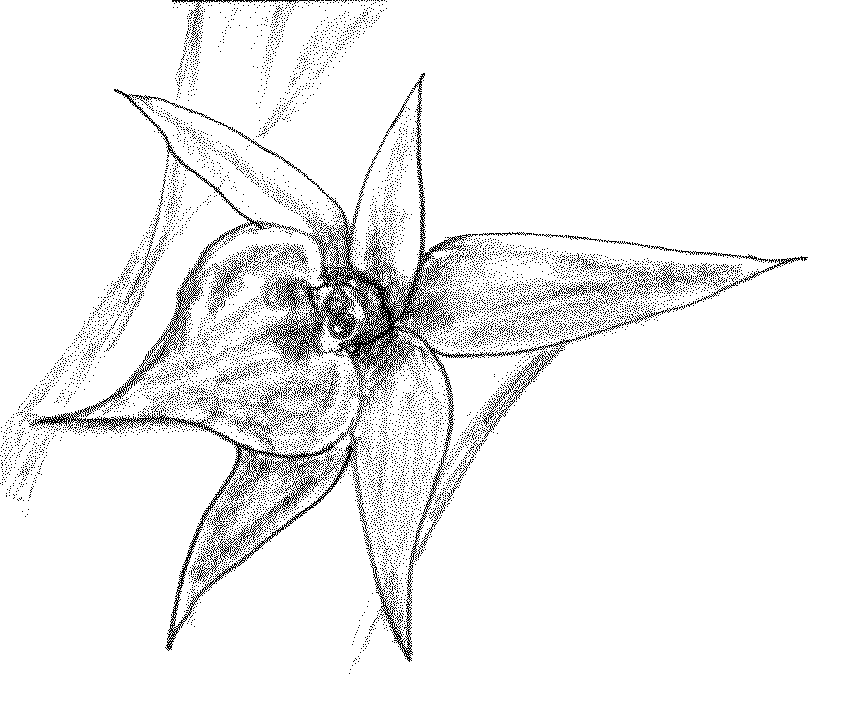
\includegraphics[width=210pt]{flower.png}
\end{center}


\chapter{Reference}

\section{Function summary}

Each of the functions, global variables, and XSLT extension elements
defined in the library is listed in this section, along with a brief
description. 

\begin{longtable}{l>{\raggedright}p{2.5cm}p{8cm}}
\it Function&\it Arguments&\it Description\\
\endhead
xmlLoadFuncs&[noinit]&Register functions with interpreter and optionally
initialise XML and XSLT libraries\\
xmlDropFuncs&&Unregister functions and shut down libraries\\
xmlVersion&&Returns the version number of the library and the XML and
XSLT libraries;\\
xmlError&&Returns the text of all error messages since most recent call;\\
xmlFree&thing, [thing2, \dots]&Releases memory associated with an object;\\

xmlParseXML&[url], [data], [flags]&Open {\it url} and parse the XML data there,
or parse {\it data}, or parse the data collected by the XML environment. Returns 0 or 
a document tree;\\
xmlParseHTML&url, [data], [flags], [encoding]&Open {\it url} and parse the HTML data,
or parse {\it data}, or parse the data collected by the XML environment.
Returns 0 or a document tree;\\
xmlSaveDoc&[url], doc, [stylesheet]&Writes the content of the document
tree {\it doc} to {\it url}, or returns it as a string.\\
xmlNodeContent&node&returns the string content of {\it node}\\
xmlExpandNode&stem, node&Populates a stem with the data from {\it
node};\\
xmlFreeDoc&doc, [\dots]&Frees one or more document tree\\
xmlEvalExpression&expr, [node], [context]&Evaluates an XPath expression
and returns the result as a string;\\
xmlFindNode&expr, [node], [context]&Evaluates an XPath expression
and returns the result as a node set;\\
xmlNodesetCount&nodeset&Returns the number of nodes in node
set {\it nodeset};\\
xmlNodesetItem&nodeset, index&Returns the {\it index}th member of node
set {\it nodeset};\\
xmlNodesetAdd&[nodeset], node, [node2,\dots]&Adds the specified nodes to
node set {\it nodeset}. Creates a new node set if none is given;\\
xmlNewContext&node, [nsdeclaration], [\dots]&Allocates and returns a new
context with context node {\it node}, and the specified name-space
prefixes registered;\\
xmlSetContext&[ctxt], [node], [nsdeclaration], [\dots]&Changes the context node
and adds new name-space declarations;\\
xmlFreeContext&[ctxt1], [\dots]&Frees one or more contexts. If no
context is given, frees the default context;\\
xmlCompileExpression&expr&Converts {\it expr} to a form which can
be applied quickly;\\
xmlFreeExpression&expr&Frees a compiled expression;\\
xmlParseXSLT&[url], [expr]&Parses and compiles an XSLT stylesheet from a URL,
a Rexx expression, or the XSLT environment\\
xmlFreeStylesheet&ss, [\dots]&Frees one or more compiled stylesheets\\
xmlApplyStylesheet&ss, doc, [ssfmt], [docfmt], [parm, value], [\dots]&Applies
the stylesheet {\it ss} to the document {\it doc}\\
xmlOutputMethod&ss&Reports the output put method of stylesheet {\it
ss};\\
xmlParseSchema&[url],[expr]&Parses the schema document contained in a
URL, a Rexx expression, or the XSD environment\\
xmlFreeSchema&xsd, [\dots]&Frees one or more schema documents;\\
xmlValidateDoc&xsd, doc, [xsdfmt], [docfmt]&Validates the document {\it
doc} according to the stylesheet {\it xsd};\\
xmlDumpSchema&file, xsd, [xsd2], \dots&Writes one or more schemas to
file {\it file}, for debug purposes\\
xmlNewDoc&&Creates a new, empty XML document tree;\\
xmlNewHTML&&Creates a new HTML document tree;\\
xmlAddElement&node, name, [text], [where]&Creates a new element and adds it as a child
of {\it node}. If {\it where} is set, the element will be added as a sibling of
{\it node}, either `before', `after', or `replacing' it;\\
xmlAddAttribute&node, name, [text]&Creates a new attribute and adds it to
{\it node}.\\
xmlAddText&node, text, [where]&Creates a text node and adds it as a child
of {\it node}. {\it Where} follows \fn{xmlAddElement}\\
xmlAddPI&node, name, [text], [where]&Creates a processing instruction
and adds it as a child of {\it node}. {\it Where} follows \fn{xmlAddElement}\\
xmlAddComment&node, [text], [where]&Creates a comment and adds it as a child of {\it node}. {\it Where} follows \fn{xmlAddElement}\\
xmlAddNode&node, child, [where]&Adds the node {\it child} as a child of {\it node}. {\it Where} follows \fn{xmlAddElement}\\
xmlCopyNode&node&Creates a new node which is a copy of {\it node}\\
xmlRemoveAttribute&node, name, [\dots]&Removes one or more attributes from
node;\\
xmlRemoveContent&node, [\dots]&Removes all the children of one or more
nodes;\\
xmlRemoveNode&node, [\dots]&Removes one or more nodes from the
document tree;\\
xmlPost&url, [data], [format], [headers], [contvar]&Sends an HTTP POST command to a URL and returns the resulting
data;\\
xmlGet&url, [contvar]&Retrieves data from a URL and returns it.\\
\end{longtable}


\section{Housekeeping routines}

These are routines which help you use the other routines.
Only \fn{xmlLoadFuncs} and \fn{xmlVersion} are exposed by the library.
One normally calls \fn{xmlLoadFuncs} to register other functions,
as described in section \ref{sec:rxfuncadd}.

\subsection{xmlLoadFuncs}

\begin{verbatim}
xmlLoadFuncs([noinit]) -> 0
\end{verbatim}

\fn{xmlLoadFuncs}\index{xmlLoadFuncs} registers all the other routines in the utility package
with the Rexx interpreter. The function needs to be called once at script
invocation time. IBM's interpreters typically have the registration
persist after the script has finished running. Other vendor's
interpreters do not do this.

If the {\it noinit} argument is passed, with any value, libxml and libxslt
are not initialised by the library. You should do this when writing macros
to be executed from programs which use those libraries themselves. By
default, libxml and libxslt are initialised by
xmlLoadFuncs(\,).\index{libxml!initialisation}\index{libxslt!initialisation}

\subsection{xmlDropFuncs}

\begin{verbatim}
xmlDropFuncs() -> 0
\end{verbatim}

\fn{xmlDropFuncs}\index{xmlDropFuncs} removes the registration of all the functions in the package
from the Rexx interpreter. I don't feel there's a compelling reason for
doing this, and it has the potential to be positively harmful in the
IBM interpreters, since they don't do proper reference counting for
load/drop. By the same token, with the IBM interpreters it may be
impossible to upgrade the library without first unloading the functions.

\subsection{xmlVersion}

\begin{verbatim}
xmlVersion() -> v.r.m xmlvn xslvn
\end{verbatim}

\fn{xmlVersion}\index{xmlVersion} returns the version number of the library,
in the format {\it version.\penalty\exhyphenpenalty release.\penalty\exhyphenpenalty
modification}, followed by the libxml version number and the libxslt version
number. This can be useful for ensuring
that an upgrade has gone successfully, or for reporting and coding around bugs
in the library.

I have historically forgotten to change the version number with some
library releases, but my current build procedure should limit the likelihood of
that happening again.

\subsection{xmlError}

\begin{verbatim}
xmlError() -> error message
\end{verbatim}

\fn{xmlError}\index{xmlError} returns the accumulated error and warning messages
since the last time \fn{xmlError} was called.
These messages are intended to assist humans in problem determination.
It's not a bad idea to call this even after a successful function call,
in case there were warning messages.

\subsection{xmlFree}

\begin{verbatim}
call xmlFree thing [, thing2, ...]
\end{verbatim}

\fn{xmlFree}\index{xmlFree} releases memory for anything that isn't a
string and doesn't have a more specific deallocator. For instance,
you'd use \fn{xmlFree} for node sets, but \fn{xmlFreeDoc} for document
trees.

\section{C Language Interface}

RexxXML is meant to be used by libxml-based programs which provide a
Rexx scripting environment. Most of the types exposed in the API
map directly to types in libxml, so it should be simple to create
variables and functions which interact cleanly with the RexxXML API.
The library exposes C functions which can be used to load and
unload the library.

\subsection{Data types}

If you're unsure of which type to use for a particular variable, check the
source code. This section says which C type I've used for each of the
Rexx return types.

The `tree representation' is an xmlDocPtr, which is a tree consisting of
various types based on xmlNodePtr. Any node taken from a tree is one of
those types. rexxxml.h defines the union xmlnodeptr\_t, which might be
helpful in situations where polymorphism is needed.

A compiled XPath expression is an xmlXPathCompExprPtr, but with `\&'
prepended to it. The rationale for this is that I needed to ensure there
was a character which was not allowed in an XPath expression to allow
me to detect the difference.

A node set is an xmlXPathObjectPtr of type XPATH\_NODESET.

An XPath context is an xmlXPathContextPtr. The context pointers
allocated by RexxXML have their own function and variable look-up
functions, so if you use a context pointer generated by your
application, the automatic mapping to Rexx variables and external
functions will not work.

A parsed XSLT stylesheet is an xsltStylesheetPtr.

A parsed Schema is an xmlSchemaPtr. We need to generate a validation
context each time we perform validation. I'm not sure if this is a problem.

\subsection{rexxXMLInit}

\begin{verbatim}
void rexxXMLInit(int initparser)
\end{verbatim}

\fn{rexxXMLInit}\index{rexxXMLInit} registers the library functions with
the Rexx processor and performs other library initialisation tasks.
If {\it initparser} is non-zero, it also calls initialisation routines
for libxml and libxslt. If your program already uses libxml,
you should set {\it initparser} to 0.

You would normally call \fn{rexxXMLInit} once during the run of your
program.

\subsection{rexxXMLFini}

\begin{verbatim}
void rexxXMLFini(void)
\end{verbatim}

\fn{rexxXMLFini}\index{rexxXMLFini} reverses the registration of all the
library functions and releases any resources acquired by the library
during its run. libxml and libxslt shutdown routines will be called
only if the {\it initparser} argument to \fn{rexxXMLInit} was non-zero.

\section{The XML, XSLT, and XSD environments}

\begin{verbatim}
address XML
'<formletter><to><name>'name'</name><address>'address'</address></to>'
'<salutation>Dear' name'</salutation>'
'<p>Thank-you for your interest in RexxXML...'
'</p></formletter>'
\end{verbatim}

RexxXML\index{XML!environment}\index{XSLT!environment}\index{XSD!environment}\index{environments}
defines\label{sec:xmlenv} environments called XML, XSLT, and XSD.
Commands issued in these environments are appended together, and can be
returned as a tree using \fn{xmlParseXML}, \fn{xmlParseHTML},
\fn{xmlParseXSLT}, and \fn{xmlParseSchema} without specifying either of
the first two arguments.  The result is exactly equivalent to appending the
data to a string and parsing the string.

You might ask, why do these environments exist? Some types of programs
are closely associated with some of their data, such that it may be
more convenient to store the data as part of the program. These
environments exist to support that type of program. If you need to
massage some data with a simple XSLT stylesheet before processing it,
you may find it convenient to store the stylesheet in the program itself.

The nature of Rexx environments limits the convenience of this approach,
since everything that gets passed to the environment has to be a valid
Rexx expression. If the embedded text is lengthy, or includes quotation
marks (almost unavoidable when dealing with XML data), creating it as
part of a script can try your patience. On the other hand, as the example
at the top of this section shows, it can be a convenient way of
integrating boilerplate with dynamic data.

Another approach which may be helpful is to achieve the same goal is to
put a document in a Rexx comment, then retrieve the text using
\fn{sourceline}. This approach doesn't work with pre-compiled scripts,
though.

\begin{verbatim}
/* PTOD
  <?xml version="1.0"?>
  <xsl:stylesheet xmlns:xsl='http://www.w3.org/1999/XSL/Transform'>
    <xsl:template match="node()|@*">
      <xsl:copy>
        <xsl:apply-templates match="node()|@*"/>
      </xsl:copy>
    </xsl:template>
    <xsl:template match="p">
      <d>
        <xsl:copy-of match="."/>
      <d>
    </xsl:template>
  </xsl:stylesheet>
PTOD */

address XSLT
sv = 0
do i = 1 to sourceline()
  parse value sourceline(i) with f1 f2
  if sv & f1 = "PTOD" & f2 = "*/" then leave
  if sv then sourceline(i)  /* sends value to the XSLT environment */
  else if f1 = "/*" & f2 = "PTOD" then sv = 1
  end
if sv then ss = xmlParseStylesheet()
else say 'no stylesheet in script'
\end{verbatim}

Note that the XML environment can be used with both \fn{xmlParseXML} and 
\fn{xmlParseHTML}.

The parse functions are the only way to clear the values stored up by the
environments.


\section{Document tree processing}

Most RexxXML processing consists of building document trees in memory,
manipulating them, and writing them out again. Several functions allow
trees to be built from existing XML data, either resident in a file,
built with an expression, or stored in the XML environment.

\subsection{xmlParseXML}

\begin{verbatim}
xmlParseXML([url], [inline], [flags]) -> node or 0
\end{verbatim}

\label{sec:xmlparsexml}\fn{xmlParseXML}\index{xmlParseXML} returns the tree representation of
an XML document. The document can be retrieved from a URL, from a
Rexx expression, or from the XML environment. {\it Url} can be a file
name, an HTTP address, or an FTP address which resolves to the document
to be processed. {\it Inline} is an expression which evaluates to an XML
document. It is ignored if {\it url} is specified. If neither {\it url}
nor {\it inline} is specified, the document is retrieved from the XML
environment. Depending on how libxml was compiled, {\it url}
can refer to a file which has been compressed using gzip, in which
case the file will be uncompressed automatically.

{\it Flags} controls the way the document is parsed, and can consist of
any combination of the letters `v', `d', and `s', in either upper- or
lower-case. If `v' is included, the parser will validate the document,
and \fn{xmlParseXML} will fail if the document does not have a document
type declaration or if it doesn't conform to the DTD. If `d' is included
and there's a document type declaration, the external subset of the DTD
will be loaded. By default, the external subset is ignored. If `s' is
included, spaces which are not meaningful in the mark-up will be
stripped out. By default, the tree representation includes text nodes
representing white space which is not allowed in the content model, but
which is required to reconstruct the input file.

If you need to go through a proxy server for HTTP or FTP requests\index{proxy
server}, set the environment variables HTTP\_PROXY or FTP\_PROXY,
respectively. The format is `{\it protocol}://{\it host}:{\it port}/', where
{\it protocol} is one of `http' or `ftp', and {\it host} and {\it port} are
the proxy server's host name and its port number. {\it Port} is optional if
the server is installed at the default port for the protocol.
The environment variables ftp\_proxy\_user and ftp\_proxy\_password
should be set if you need to use a password for your ftp proxy server.

\subsection{xmlNewDoc}

\begin{verbatim}
xmlNewDoc([version], [encoding]) -> node or 0
\end{verbatim}

Creates a new, empty document tree and returns\index{xmlNewDoc} the root
node. A document can be built by adding nodes using the \fn{xmlAdd*}
and \fn{xmlCopyNode} functions.

{\it Version} is the XML version number. The default is 1.0.

{\it Encoding} is the encoding. The default is UTF-8. The ISO 8-bit
character sets are available as ISO-8859-{\it n}, where {\it n} is the
code-page number.

\subsection{xmlParseHTML}

\begin{verbatim}
xmlParseHTML([url], [inline], [flags], [encoding]) -> node or 0
\end{verbatim}

Parses HTML data, which can be loaded from a URL, a Rexx expression,
or the XML environment. See section \ref{sec:xmlparsexml} for details of
the {\it url}, {\it inline}, and {\it flags} arguments.

{\it Encoding} is the character set of the data. The default value is
ISO-8859-1.


\subsection{xmlNewHTML}

\begin{verbatim}
xmlNewHTML([publicID], [systemID]) -> node or 0
\end{verbatim}

Creates\index{xmlNewHTML} a new, empty HTML document tree and returns\index{xmlNewHTML} the root
node. A document can be built by adding nodes using the \fn{xmlAdd*}
and \fn{xmlCopyNode} functions.

{\it PublicID} is the public identifier for the document type
declaration. The default is `-//W3C//DTD HTML 4.01 Transitional//EN'.

{\it SystemID} is the system identifier for the document type
declaration. The default is to have no default.

\subsection{xmlSaveDoc}

\begin{verbatim}
xmlSaveDoc(url, doc, [stylesheet]) -> length or 0
xmlSaveDoc(, doc, [stylesheet]) -> text or 0
\end{verbatim}

\fn{xmlSaveDoc}\index{xmlSaveDoc} converts an XML or HTML
document tree, {\it doc}, to a string, and either writes that string to the URL {\it url},
or returns it. If {\it url} is specified, the return code
is the length of the data that was written to the URL.

If {\it doc} is the result of an XSLT transformation, you should pass the
compiled stylesheet as {\it stylesheet}. This is necessary to get correct
output when the output method is `text', and it's probably a good idea
for other transformations.



\subsection{xmlFreeDoc}

\begin{verbatim}
call xmlFreeDoc doc [, doc2, ...]
\end{verbatim}

\fn{xmlFreeDoc}\index{xmlFreeDoc}Releases the memory resources
associated with one or more XML or HTML document trees. {\it Doc}
is the output of \fn{xmlParseXML}, \fn{xmlParseHTML}, \fn{xmlNewDoc},
or \fn{xmlNewHTML}. You may specify as many document pointers as
you like. There's no performance advantage to this, I just think it's
more readable to have one `free' call with several arguments than to
have several `free' calls with one argument.

\subsection{xmlExpandNode}

\begin{verbatim}
xmlExpandNode(stemname, node) -> 0 or 1
\end{verbatim}

\label{sec:nodedef}\fn{xmlExpandNode}\index{xmlExpandNode} converts a
node from the tree representation of an XML or HTML document into a
Rexx compound variable.\index{variable!compound}
There's currently no way to convert this compound variable back into
a node. The stem is dropped before any of the tails listed below is set.
The function returns 1 if the conversion was successful, or 0
otherwise.

The best way to get a feel for the compound variable structure is to run
the example script dumpfile.rex over some documents, as discussed
in section \ref{sec:dumpfile}. This calls the
external routine treewalk\index{treewalk.rex} which can be useful in
debugging problems with the file structure (for instance, if you
want to know why your XPath expressions aren't working) (not that this
has happened to me).

There are several different types of nodes, with different types having
different data associated with them. There are some common tails, and
some which depend on the node type. In general, the values are either
strings which can be processed directly by the Rexx program or nodes,
which can be passed to RexxXML functions.

\subsubsection{Tails common to all nodes}

These tails can occur with any node. Some of them are text values, while
others are nodes themselves. Nodes which have no value are set to 0.

In some cases, the tails might not be set. \fn{Symbol} can be used 
to determine whether a variable has been set or not.

\begin{enumerate}
\item[TYPE]The type of node. The types are ELEMENT\_NODE (an element), ATTRIBUTE\_NODE (an
attribute value), TEXT\_NODE (a text node), CDATA\_SECTION\_NODE (a text node,
but possibly with illegal characters), ENTITY\_REF\_NODE (an entity
reference~-- the data appears as a child of this), ENTITY\_DECL (an
entity declaration in a DTD), ENTITY\_NODE (I haven't seen this~-- possibly
it's for unparsed entities or entities in attribute values),
PI\_NODE (a processing instruction), COMMENT\_NODE (a comment), HTML\_DOCUMENT\_NODE (the
root of an HTML document), DOCUMENT\_NODE (the root of an XML document),
DOCUMENT\_TYPE\_NODE (document type declaration~-- I haven't seen this), DOCUMENT\_FRAG\_NODE (the root of a
document fragment, which I don't think can happen with the routines in this library),
NOTATION\_NODE (a notation declaration), DTD\_NODE (a document type
declaration),
ELEMENT\_DECL (an element declaration, ATTRIBUTE\_DECL (an attribute
declaration), and NAMESPACE\_DECL (a name-space declaration)
\item[NAME]The name of the node. This has meaning for elements,
attributes, PIs, entities, {\it \&c}.. It might not be set for other types;
\item[SELF]The node itself
\item[CONTENT]The text content of the node. This has meaning for text
nodes and a few other types, and is not set for the others. In element
declarations, {\it content} gives the content model. In attribute
declarations, it gives the default value.
The data is always encoded in UTF-8;
\item[NEXT]The next sibling node, or 0
\item[PREV]The previous sibling node, or 0
\item[CHILDREN]The first child node, or 0
\item[LAST]The last child node, or 0
\item[PARENT]The parent node
\item[ATTRIBUTES]The attributes of this element, or 0
\item[EXTERNALID]The external part of a public identifier. It might
not be set;
\item[SYSTEMID]A system identifier. It might
not be set;
\item[NAMESPACEPREFIX]The name-space prefix for this element or attribute. It might
not be set;
\item[NAMESPACEURL]The name-space URL for this element or attribute. It might
not be set
\end{enumerate}

\subsubsection{Tails specific to document nodes}

\begin{enumerate}
\item[COMPRESSION]The level of compression at which {\it doc} is to be
saved, or $-1$ if no compression level has been set;
\item[STANDALONE]1 if the document has no external references, or 0
if it does;
\item[INTSUBSET]The first node of the internal subset, or 0
\item[EXTSUBSET]The first node of the external subset, or 0
\item[VERSION]The XML version number required by the document (1.0);
\item[ENCODING]The encoding of the document. Text is always returned
by the library in UTF-8.
\end{enumerate}

\subsubsection{Tails specific to attribute nodes}

`AType' is set for both attribute values and attribute declarations.
`Mandatory' is set only for attribute declarations.

\begin{enumerate}
\item[ATYPE]The attribute type, each of these values corresponds to a type in
the table on page \pageref{page:attrtype}. The possible values are
ATTRIBUTE\_CDATA, ATTRIBUTE\_ID, ATTRIBUTE\_IDREF, ATTRIBUTE\_IDREFS,
ATTRIBUTE\_ENTITY, ATTRIBUTE\_ENTITIES, ATTRIBUTE\_NMTOKEN,
ATTRIBUTE\_NMTOKENS, ATTRIBUTE\_ENUMERATION, and ATTRIBUTE\_NOTATION
\item[MANDATORY]One of ATTRIBUTE\_NONE, ATTRIBUTE\_REQUIRED,
ATTRIBUTE\_IMPLIED, or ATTRIBUTE\_FIXED.
\end{enumerate}

\subsubsection{Tails specific to element declarations}

\begin{enumerate}
\item[ETYPE]Type type of content, one of ELEMENT\_TYPE\_UNDEFINED,
ELEMENT\_TYPE\_EMPTY, ELEMENT\_TYPE\_ANY, ELEMENT\_TYPE\_MIXED, or
ELEMENT\_TYPE\_ELEMENT
\end{enumerate}

\subsubsection{Tails specific to element nodes}

\begin{enumerate}
\item[A]The names of each attribute which was explicitly set for this
instance of the element, converted to upper-case and space-delimited;
\item[A.{\it attr}]The value of attribute {\it attr} for this instance
of the element. {\it Attr} is converted to upper-case to allow it
to be typed directly as in `stem.a.name'. The attribute value is presented
as a string with all entity references resolved. The attributes
tail can be used to  access the attributes as a set of nodes
\end{enumerate}

\subsubsection{Tails specific to entity declarations}
\begin{enumerate}
\item[ETYPE]The type of entity, as discussed in section \ref{sec:entdecl}. The
possible values are INTERNAL\_GENERAL\_ENTITY,
EXTERNAL\_GENERAL\_PARSED\_ENTITY, EXTERNAL\_GENERAL\_UNPARSED\_ENTITY,
INTERNAL\_PARAMETER\_ENTITY, EXTERNAL\_PARAMETER\_ENTITY, or
INTERNAL\_PREDEFINED\_ENTITY
\end{enumerate}

\subsection{xmlNodeContent}

\begin{verbatim}
xmlNodeContent(node) -> string or ''
\end{verbatim}

\index{xmlNodeContent}\index{getting!text content of nodes}\fn{xmlNodeContent}
returns the value of all the text nodes which are descendants of {\it node},
concatenated together. If there's an error, it returns the empty string.

\subsection{xmlAddElement}

\begin{verbatim}
xmlAddElement(node, name, [text], [where]) -> 0 or newnode
\end{verbatim}

\index{xmlAddElement}\fn{xmlAddElement} creates a new element called
{\it name} and adds it to a document as either a child or sibling of
{\it node}. It returns the new node on success, or 0 on failure.

If {\it text} is set, it is added as content of the new node.

The default behaviour is to add the new element to the end of the list
of children of {\it node}.
If {\it where} is set, the new node is added as a sibling of {\it node}.
Only the first character is tested, but the valid values are meant to be
`before', `after', or `replace'. The effect of these values is,
respectively, to add the new node just before {\it node}, just after
{\it node}, or in place of {\it node}.

\label{sec:addelement}Here are some examples\index{hoping to avoid
confusion}
\begin{verbatim}
doc = xmlParseXML(,'<data><a><b/></a></data>')
call xmlexpandNode 'x.', doc
call xmlexpandNode 'x.', x.children
a = x.children      /* node <a> */
c = xmlAddElement(a, 'c')
/* doc = <data><a><b/><c/></a></data> */
d = xmlAddElement(c, 'd', 'text', 'replace')
/* doc = <data><a><b/><d>text</d></a></data> */
e = xmlAddElement(d, 'e',, 'before')
/* doc = <data><a><b/><e/><d>text</d></a></data> */
f = xmlAddElement(d, 'f',, 'a')
/* doc = <data><a><b/><e/><d>text</d><f/></a></data> */
\end{verbatim}

\subsection{xmlAddAttribute}

\begin{verbatim}
xmlAddAttribute(node, name, [value]) -> newnode or 0
\end{verbatim}

\index{xmlAddAttribute}\fn{xmlAddAttribute} sets the attribute {\it name}
for node {\it node} to the value {\it value}. {\it Node} must be an
element node. If the attribute is already set, its value is replaced.
If {\it value} is not specified, the attribute is set to a zero-length
string. Use \fn{xmlRemoveAttribute} to remove an attribute from an
element.

\subsection{xmlAddText}

\begin{verbatim}
xmlAddText(node, text, [where]) -> newnode or 0
\end{verbatim}

\index{xmlAddText}\fn{xmlAddText} adds the text {\it text} as a child of
node {\it node}, and returns the new text node.
{\it Where} has the same meaning as for \fn{xmlAddElement}, which is
described in section \ref{sec:addelement}.

\subsection{xmlAddPI}

\begin{verbatim}
xmlAddPI(node, name, [text], [where]) -> 0 or newnode
\end{verbatim}

\index{xmlAddPI}\fn{xmlAddPI} creates a new processing instruction with name
{\it name} and adds it to a document as either a child or sibling of
{\it node}. It returns the new node on success, or 0 on failure.

If {\it text} is set, it is placed after the name in the processing
instruction. Although processing instructions defined by the world-wide
web consortium tend to look like elements with attribute values, this is
an illusion~-- {\it text} is free-form, and RexxXML does nothing
to support its formatting.

{\it Where} has the same meaning as for \fn{xmlAddElement}, which is
described in section \ref{sec:addelement}.

\subsection{xmlAddComment}

\begin{verbatim}
xmlAddComment(node, text, [where]) -> newnode or 0
\end{verbatim}

\index{xmlAddComment}\fn{xmlAddComment} adds a comment, with {\it text} as its content,
as a child of node {\it node}, and returns the new comment node.
It seems common for applications to store processing instructions in
comments, and I'd like to take this opportunity to say that there doesn't
seem to be any benefit to this. You should use PIs to pass information
to programs and comments to pass
information to human readers.

{\it Where} has the same meaning as for \fn{xmlAddElement}, which is
described in section \ref{sec:addelement}.

\subsection{xmlAddNode}

\begin{verbatim}
xmlAddNode(node, newnode, [where]) -> newnode or 0
\end{verbatim}

\index{xmlAddNode}\fn{xmlAddNode} adds {\it newnode} as a child
of node {\it node}, and returns {\it newnode}. This can be useful
in conjunction with \fn{xmlCopyNode} to move a node from one
document to another.

{\it Where} has the same meaning as for \fn{xmlAddElement}, which is
described in section \ref{sec:addelement}.

\subsection{xmlCopyNode}

\begin{verbatim}
xmlCopyNode(node) -> newnode or 0
\end{verbatim}

\index{xmlCopyNode}\fn{xmlCopyNode} creates a copy of the node {\it
node} and its children. This copy can be added to a different place in the
document tree using \fn{xmlAddNode}.

\subsection{xmlRemoveAttribute}

\begin{verbatim}
call xmlRemoveAttribute node, name, [name2], [...]
\end{verbatim}

\index{xmlRemoveAttribute}\fn{xmlRemoveAttribute} unsets the attributes
called {\it name}, {\it name2} and so forth from the node {\it node}.
More than one attribute name can be specified per call, because I think
this leads to more readable code. There's no harm in calling it once
for each attribute, and there's no harm in calling it for attributes
which are not set.

\subsection{xmlRemoveContent}

\begin{verbatim}
call xmlRemoveContent node, [node2], [...]
\end{verbatim}

\index{xmlRemoveContent}\fn{xmlRemoveContent} removes all the child
nodes from the specified nodes, which might be useful if you want to
replace the text content of a node. You must be careful not to use
a node value after it has been released in this way.

\subsection{xmlRemoveNode}

\begin{verbatim}
call xmlRemoveNode node, [node2], [...]
\end{verbatim}

\index{xmlRemoveNode}\fn{xmlRemoveNode} removes all the specified  nodes and their
child nodes from the document tree. You must be careful not to use
a node value which has been released in this way.


\section{Document tree searching}

The functions in this section provide an interface to XPath expressions.
The way they fit together is discussed at some length in section
\ref{sec:usexpath}.

\subsection{xmlEvalExpression}

\begin{verbatim}
xmlEvalExpression(expr, [node], [context]) -> string or ''
\end{verbatim}

\index{xmlEvalExpression}\fn{xmlEvalExpression} evaluates
the expression {\it expr} and returns the result as a string.
If {\it expr} returns a node set, the string value is the value
of all the text nodes which are in the node set or are descendants of the
nodes in the node set, concatenated together. {\it Expr} can be a
string, or it can be the return code of \fn{xmlCompileExpression}.

If {\it node} is specified, it is used as the context node for the
evaluation, and it sets the context node for the evaluation context.
Otherwise, the context node is taken from the evaluation
context.

{\it Context} is an evaluation context to use for the evaluation.
It might be the return code of \fn{xmlNewContext}, the value of
the {\it xmlContext} variable in a script called from XSLT,
or a context obtained in some other way from the calling
application. If {\it context} is not specified, a default
context is used.

With either the default context or a context returned by
\fn{xmlNewContext}, variables evaluate to Rexx variables
of the same name and unrecognised functions are mapped to
Rexx external functions. On systems with case-sensitive file systems,
the function name used in the XPath expression must match the case of
the external function's file name.

\subsection{xmlFindNode}

\begin{verbatim}
xmlFindNode(expr, [node], [context]) -> nodeset or 0
\end{verbatim}

\index{xmlFindNode}\fn{xmlFindNode} evaluates
the expression {\it expr} and returns the result as a node set.
The arguments are the same as for \fn{xmlEvalExpression}, except
that {\it expr} must evaluate to a node set.

\subsection{xmlNodesetCount}

\begin{verbatim}
xmlNodesetCount(nodeset) -> number
\end{verbatim}

\index{xmlNodesetCount}Given a node set {\it nodeset},
\fn{xmlNodesetCount} returns the number of nodes in the set. It returns
0 either if there are no nodes in the set, or if {\it nodeset} is an
XPath value, but not a node set.

\subsection{xmlNodesetItem}

\begin{verbatim}
xmlNodesetItem(nodeset, n) -> node or 0
\end{verbatim}

\index{xmlNodesetItem}\fn{xmlNodesetItem} returns the {\it n}th node
from node set {\it nodeset}, where the nodes are numbered starting
at 1. If {\it n} is out of bounds, the function returns 0.

\subsection{xmlCompileExpression}

\begin{verbatim}
xmlCompileExpression(expr) -> cexpr or 0
\end{verbatim}

\index{xmlCompileExpression}\fn{xmlCompileExpression} converts the
string expression {\it expr} into a form which can be evaluated quickly. The return
code can be passed to either \fn{xmlEvalExpression} or \fn{xmlFindNode}.
The compiled expression is useful only for the duration of the process
in which it was created. It cannot be stored and reused by another process.

The performance improvement provided by using compiled expressions is
measurable, but small. It makes sense to use them whenever an expression
must be evaluated repeatedly during the run of one program.

\subsection{xmlFreeExpression}

\begin{verbatim}
call xmlFreeExpression cexpr, [cexpr2], [...]
\end{verbatim}

\index{xmlFreeExpression}\fn{xmlFreeExpression} releases the memory
associated with one or more compiled expressions {\it cexpr}. You
should release all the expressions you compile at the point where
you no longer need them.

More than one expression can be passed in a single call of this function.

\subsection{xmlNewContext}

\begin{verbatim}
xmlNewContext(node,[namespace],[...]) -> context or 0
\end{verbatim}

\index{xmlNewContext}\fn{xmlNewContext} allocates a new XPath evaluation
context and sets the context node to {\it node}. If any {\it namespace}
arguments are given, they must have the form `prefix=url', and they
\label{sec:newcontext}are used to set name-space prefixes for the evaluation context.

It makes sense to allocate new evaluation contexts if you are continuously
switching between searches based on different documents or different
name-spaces.

The context node can be changed using \fn{xmlSetContext} or the {\it
node} argument to \fn{xmlEvalExpression} or \fn{xmlFindNode}. When
you've finished with an evaluation context, you should release it using
\fn{xmlFreeContext}.

\subsection{xmlSetContext}

\begin{verbatim}
xmlSetContext([context], node, [namespace], [...]) -> 0 or 1
\end{verbatim}

\index{xmlSetContext}\fn{xmlSetContext} sets the context node
for and adds name-space prefixes to the specified evaluation context.
If {\it context} is not given, \fn{xmlSetContext} affects the default
context. The {\it namespace} arguments are as described in section
\ref{sec:newcontext}.

\subsection{xmlFreeContext}

\begin{verbatim}
call xmlFreeContext [context], [context2], [...]
\end{verbatim}

\index{xmlFreeContext}\fn{xmlFreeContext} releases the memory
associated with one or more evaluation contexts. If no arguments
are given, the default context is released. This is the only way
to unset name-space prefixes in the default context.

With the exception of the default context, which is reallocated as
needed, you must be careful not to use a context after it has been
released.

More than one context can be passed in a single call of this function.

\subsection{xmlNodesetAdd}

\begin{verbatim}
xmlNodesetAdd([nodeset], [node], [node2], [...]) -> nodeset
\end{verbatim}

\index{xmlNodesetAdd}\fn{xmlNodesetAdd} either adds the given {\it node}s to the
existing node set {\it nodeset}, or it creates a new node set and adds
the {\it node}s to it. If there are no arguments, \fn{xmlNodesetAdd}
creates a new, empty node set.

This function is meant to allow you to create new XPath functions which
return node sets.

\subsection{XPath Environment}

\begin{verbatim}
trace 'o'
address xpath
'//nodename'
\end{verbatim}

The XPath environment\index{XPath!environment} evaluates commands against
the default context. You should call \fn{xmlSetContext} to establish the
context node before using the environment.

\section{XSLT processing}

RexxXML includes functions for invoking an XSLT processor to transform a
document. The stylesheets invoked using RexxXML can use extension elements to
embed Rexx scripts in the stylesheet. This gives access to Rexx's
arbitrary-precision arithmetic and string manipulation instructions, as well
as a wide range of function libraries and operating system commands.

The full range of RexxXML functions is available from these embedded scripts,
but variables from the Rexx script which invoked the XSLT stylesheet are not
available to functions or scripts called from the stylesheet. They are all
effectively external functions. You can pass data using \fn{value}, setting
the third argument to `ENVIRONMENT'.

To use the extension elements, you must declare a name-space prefix with the
URL urn://rexxxml\slash xslt and add it to the list of
extension-element-prefixes. These declarations are normally done as part of
the stylesheet element, but the synopses show it being done as part of the
Rexx scripts themselves.

\subsection{xmlParseXSLT}

\begin{verbatim}
xmlParseXSLT([url], [inline]) -> 0 or ssp
\end{verbatim}

\fn{xmlParseXSLT}\index{xmlParseXSLT} returns a compiled version of
a stylesheet, which can be retrieved from a URL, from a
Rexx expression, or from the XSLT environment. {\it Url} can be a file
name, an HTTP address, or an FTP address which resolves to the stylesheet
to be processed. {\it Inline} is an expression which evaluates to an XSLT
stylesheet. It is ignored if {\it url} is specified. If neither {\it url}
nor {\it inline} is specified, the stylesheet is retrieved from the XSLT
environment.

The resulting stylesheet can be passed to \fn{xmlApplyStylesheet}. It
makes sense to do this if you need to apply the same stylesheet
to many documents.
The compiled stylesheet is valid only for the duration of the process
which called \fn{xmlParseXSLT}.

\subsection{xmlFreeStylesheet}

\begin{verbatim}
call xmlFreeStylesheet ssp, [ssp2], [...]
\end{verbatim}

\index{xmlFreeStylesheet}\fn{xmlFreeStylesheet} releases the memory
associated with the compiled stylesheets {\it ssp}, {\it ssp2}, {\it \&c}.

\subsection{xmlApplyStylesheet}

\begin{verbatim}
xmlApplyStylesheet(ss, doc, [ssfmt], [docfmt], [parm, value], [...]) -> doc2 or 0
\end{verbatim}

\label{sec:xmlapplystylesheet}\index{xmlApplyStylesheet}\fn{xmlApplyStylesheet} applies the stylesheet
{\it ss} to the document {\it doc} and returns the result tree. The
result tree is not guaranteed to represent a well-formed XML document.

{\it Ss} can be either a URL to the stylesheet or a compiled stylesheet
as returned by \fn{xmlParseXSLT}. Similarly, {\it doc} can be either
a URL to the document, or a document tree as returned by \fn{xmlParseXML}.
{\it Ssfmt} and {\it docfmt} are used to indicate the format of {\it ss}
and {\it doc}, respectively. The values are `url' or `tree', indicating
that the corresponding document is a URL or a parsed form, respectively.
Only the first character of the format parameters is used.
If {\it ssfmt} and {\it docfmt} are not specified, the document
arguments are expected to be trees.

Parameters can be passed to the stylesheet by specifying their names
and values starting at the fifth argument. {\it Parm} is the name of
a top-level parameter set using xsl:param, while {\it value} is the
value to use for that parameter. There must be a value for every
parameter name.

Many XSLT processors treat parameter values as XPath expressions. This
means that numbers are treated as numbers, but strings are treated as
syntax errors or empty node sets or unless you remember to put quotes
around them. Most parameter values passed to \fn{xmlApplyStylesheet}
are turned into string expressions automatically. There are three
exceptions which are treated as XPath expressions: numbers consisting of
an optional leading \verb$-$, the digits, and one optional decimal; strings
which start and end with either \verb+'+ or \verb+"+; and the values
`\fn{true}' or `\fn{false}'.

The exceptions exist to allow parameters to be set to numeric or Boolean
values, and to allow numbers to be passed as strings. The data type is important
if you want to use the parameter in certain contexts, especially in an XPath predicate.

The table shows some parameter values and the value and type to which the
parameter will be set:

\begin{longtable}{lll}
\it Argument value&\it Type&\it Parameter value\\
\endhead
27.3&Number&27.3\\
10.0.0.1&String&10.0.0.1\\
true()&Boolean&true\\
'27.3'&String&27.3\\
'hello' "there"&String&'hello' "there"\\
+82&String&+82\\
potential&String&potential\\
\end{longtable}

\subsection{xmlOutputMethod}

\begin{verbatim}
xmlOutputMethod(ss) -> string
\end{verbatim}

\index{xmlOutputMethod}The result of applying a stylesheet is a document
tree, regardless of the output method specified in the stylesheet. \fn{xmlOutputMethod}
reports the output method specified in the stylesheet, so that the output
can be generated appropriately. {\it ss} is a stylesheet returned by
\fn{xmlParseXSLT}. The output will normally be `text', `html', or `xml'.

The appropriate output processing will normally be done if the result
tree is converted to text using \fn{xmlSaveDoc} with the stylesheet
passed as the third argument.

\subsection{rexx:rexx}

\begin{verbatim}
<rexx:rexx xmlns:rexx='urn://rexxxml/xslt'
   xsl:extension-element-prefixes='rexx'>
   /* a rexx program goes here */
</rexx:rexx>
\end{verbatim}

rexx:rexx\index{rexx:rexx}\label{sec:rexx:rexx} is an element which can
appear as a child of xsl:stylesheet. It defines a Rexx script which will
be invoked each time the stylesheet is parsed.
The intent is for this script to register external procedures or
what-not, rather than being used to populate the result tree.

The contents are passed as-is to the Rexx interpreter. If you need to use
problematic characters such as \verb+<+ or \verb+&+, you may want to
include the script in a CDATA section

\begin{verbatim}
<rexx:rexx>
 <[CDATA[
    if something() & somethingelse() then call do_something
]]>   
</rexx:rexx>
\end{verbatim}

\noindent The alternative is to use entity references for those
characters, which will tend to reduce the readability of your scripts.

\subsection{rexx:function}

\begin{verbatim}
<rexx:function xmlns:rexx='urn://rexxxml/xslt'
   name='<prefix>:<name>' [return-type='<type>']  [all-strings='<bool>']
   xmlns:<prefix>='<uri>'>
   /* a rexx program goes here */
   return <value>
</rexx:function>
\end{verbatim}

rexx:function\index{rexx:function}\label{sec:rexx:function} is an element which can
appear as a child of xsl:stylesheet. It defines a function which can be called
as part of any XPath expression. The attribute `name' is required. {\it
prefix} is a name-space prefix for your function, while {\it name} is
the function name itself. Both parts are required. In any XPath
expression in the stylesheet, the function can be invoked as {\it
prefix:name}({\it arguments}).

{\it type} is the return type of the function, which can be one of `number',
`Boolean', `node set', `tree', or `string'. If the `return-type' attribute is
not specified, the return type is taken to be `string'. You need to specify a
return type\index{data types!and rexx:function} if you want to return a node set or a tree of nodes, or if you
want to use the function in a context where the return code must be seen as a
number or Boolean value by XPath. For instance, in a location step
predicate\index{number!different from string}, the string `2' is
equivalent to `\fn{true}', which will select every node matching the rest of
the location step, while the number 2 matches only the second node in the set.
Similarly, the string `false' is equivalent to \fn{true}, while the Boolean
value `false' is really \fn{false}.

For functions returning number and string, the return value is simply
the number or string you want to return. For Boolean functions, the
return value is one of `true', `on', `yes', `y', or `1' to return
\fn{true}, or any other value to return \fn{false}.
For the other return types, the return value is the appropriate
type.

Arguments to rexx:function-defined functions can be accessed as
described in section \ref{sec:arguments} on page \pageref{sec:arguments}.
By default, scalar values are available as string values (`true' or
`false' for Booleans, the normal text representation for string and
number arguments), while node set and tree arguments are passed
as node sets and trees. This can be problematic when the goal is to
examine the string value of a node. All arguments will be converted
to strings automatically if the `all-strings' attribute is set
to `true'.

In addition to the RexxXML name-space, you must declare a name-space prefix
with a URL specific to your application~-- this is the prefix that
goes in front of your function.

As with rexx:rexx, the contents are passed as-is to the Rexx interpreter.

\begin{verbatim}
<rexx:function name="ext:now">
   /* report the current date and time */
   return date() time()
</rexx:function>

<rexx:function name="ext:is-user-table" return-type='Boolean'
               all-strings='yes'>
   /* return true for arguments which start with USER_, and
    * false for the others */
   return left(arg(1), 5) = 'USER_'

   /* which could have been
   if left(arg(1), 5) = 'USER_' then return 'true'
   else return 'false'
   */
</rexx:function>

<xsl:template match="/">
  <xsl:comment>Generated on <xsl:value-of select="ext:now()"/>.</xsl:comment>
  <xsl:apply-templates/>
</xsl:template>

<xsl:template match="table[ext:is-user-table(.)]">
   <usertable><xsl:value-of select="."/></usertable>
</xsl:template
\end{verbatim}

\subsection{rexx:template}

\begin{verbatim}
<rexx:template xmlns:rexx='urn://rexxxml/xslt'
   xsl:extension-element-prefixes='rexx'
   [all-strings='<Boolean>']
   [return-type='<type>']
   [<var>='<value>' ...]>
   /* a rexx program goes here */
</rexx:template>
\end{verbatim}

rexx:template\index{rexx:template}\label{sec:rexx:template} is an element which can
appear as template content. It defines a Rexx script which will
be invoked each time the template is evaluated. If the script has a
return value, it is added to the result tree.

{\it type} is the return type of the script, which only needs to be
specified (as `tree') if you want to return a node tree. Other values are
simply cast to strings.

Values can be passed into rexx:template in two ways: through variables
or through interpolation. Any unrecognised
attributes of the rexx:template element are taken to be variable
initialisations. The attribute values accept attribute value templates (see
section \ref{sec:templatecontent}), so Rexx variables can be initialised
to the value of any XPath expression. The variables will have the
type\index{data types!and rexx:template} of the XPath expression unless the `all-strings' attribute is set
to `true'. See section \ref{sec:rexx:function} for a discussion of this.

In contrast to rexx:rexx and rexx:function, the contents of
rexx:template are applied to the current node, interpolating the
results of XSLT element evaluation with Rexx code, and the result is passed
to the Rexx interpreter. This means that rexx:template can be used as a
template for a Rexx script, which will be evaluated in the context
of an XSLT template. From a performance perspective, I haven't been
able to measure a difference between initialising a variable with
an attribute value template:
\begin{verbatim}
<rexx:template name='{name()}'>
   return name 'backwards is' reverse(name)'!'
</rexx:template
\end{verbatim}
\noindent and using interpolation:
\begin{verbatim}
<rexx:template>
   return '<xsl:value-of select="name()"/>name backwards is' ,
          reverse('<xsl:value-of select="name()"/>')'!'
</rexx:template
\end{verbatim}

\noindent The first script will be parsed only once each time the stylesheet is
used, while the second will be parsed each time the template is applied.
On the other hand, the Rexx interpreter has to evaluate the variable {\it
name} twice and perform three concatenations in the first case, but
the second expands to
\begin{verbatim}
return 'something backwards is' reverse('something')'!'
\end{verbatim}
\noindent which evaluates no variables and performs only two concatenations.
There may be a difference in performance between the two, but
so far I haven't been able to measure it.

To me, the deciding factor is that the first script is clear, whilst the
second is confusing, although it could easily be worse (it would work
equally well if the double-quotes were single-quotes). I suggest using
interpolation only in cases where you want to use flow control to
generate repetitive Rexx statements.

\section{Schema validation}

RexxXML provides limited support for XML Schemas. One can validate a document
according to a schema, but that's all. Future versions will provide a
mechanism for determining the structure of a document from a schema, and for
validating individual elements and attributes. Also, there will be some
mechanism for handling xs:appinfo elements.

\subsection{xmlParseSchema}

\begin{verbatim}
xmlParseSchema([url], [inline]) -> 0 or xsd
\end{verbatim}

\fn{xmlParseSchema}\index{xmlParseSchema} returns a compiled version of a
schema, which can be retrieved from a URL, from a Rexx expression, or from the
XSD environment. {\it Url} can be a file name, an HTTP address, or an FTP
address which resolves to the schema to be processed. {\it Inline} is an
expression which evaluates to a schema It is ignored if {\it url} is
specified. If neither {\it url} nor {\it inline} is specified, the stylesheet
is retrieved from the XSD environment.

The resulting schema can be passed to \fn{xmlValidateDoc}. It makes sense to
do this if you need to validate a number of documents using the same schema.
The compiled schema is valid only for the duration of the process which called
\fn{xmlParseSchema}.

\subsection{xmlValidateDoc}

\begin{verbatim}
xmlValidateDoc(xsd, doc, [xsdfmt], [docfmt]) -> status
\end{verbatim}

\index{xmlValidateDoc}\fn{xmlValidateDoc} validates the document {\it doc}
against the schema {\it xsd} and returns `OK' if the document is OK.
Otherwise, it returns some other string, which might be one of NOROOT,
UNDECLAREDELEM, NOTTOPLEVEL, MISSING, WRONGELEM, NOTYPE, NOROLLBACK,
ISABSTRACT, NOTEMPTY, ELEMCONT, HAVEDEFAULT, NOTNILLABLE, EXTRACONTENT,
INVALIDATTR, INVALIDELEM, NOTDETERMINIST, CONSTRUCT, INTERNAL, NOTSIMPLE,
ATTRUNKNOWN, ATTRINVALID, VALUE, or FACET. Call \fn{xmlError} to get useful
information about the cause of the error.

As with \fn{xmlApplyStylesheet}, {\it xsd} and {\it doc} can be either URLs or
parsed representations of the appropriate type of file. {\it Xsdfmt} and {\it
docfmt} can be set to `url' to indicate that the corresponding document
argument is a URL, or `tree' to indicate that the document argument is a
parsed representation of a document. If {\it xsdfmt} and {\it docfmt} are not
specified, the document arguments are expected to be trees.

\subsection{xmlFreeSchema}

\begin{verbatim}
call xmlFreeSchema xsd, [xsd2], [...]
\end{verbatim}

\index{xmlFreeSchema}\fn{xmlFreeSchema} releases the memory associated with
the compiled schemas {\it xsd}, {\it xsd2}, {\it \&c}.

\subsection{xmlDumpSchema}

\begin{verbatim}
call xmlDumpSchema file, xsd
\end{verbatim}

\index{xmlDumpSchema}\fn{xmlDumpSchema} is a debug function which dumps the
parsed schema {\it xsd} to the file {\it file}. The format of the dump is
meant to be roughly human readable, but it is undocumented and internal to
libxml. If you use it to work around the lack of any functions for determining
the structure of a schema, you should be prepared for the format to change
between versions of libxml.

\section{HTTP and FTP}

libxml contains client library for FTP and HTTP access. RexxXML exposes
functionality which is meant to be sufficient for normal processing
of web data, in particular, sending data to an HTTP server
and fetching non-XML data from either an HTTP or an FTP server.

\subsection{xmlPost}

\begin{verbatim}
xmlPost(url, [data], [format], [headers], [contvar]) -> return data
\end{verbatim}

\fn{xmlPost}\index{xmlPost} sends data to an HTTP server using the
HTTP POST method. {\it Data} is the data to be posted. {\it Format}
is the format of that data. {\it Headers} is a series of newline-delimited
HTTP headers not including `Content-type' or `Content-length', which will
be put at the start of the post. {\it Contvar} is the name of a variable
which will be set with the content type of the return data.

The data that you send and receive depends on the software which will
process it, but ordinarily I expect this routine to be used post data
associated with an HTML form, and for it to be processed by a CGI program
on the server side. The default {\it type} is
'application/x-www-form-urlencoded', which is correct for this use.
For this use, {\it data} should consist of ${\it name}={\it value}$
pairs, where {\it name} is the value of the `name' attribute of an
HTML `input' element, and value has certain special characters
replaced by their hexadecimal values. To be safe, you could replace
all but ascii letters and digits with their hexadecimal values,
preceded by a per-cent sign (\%). Simple spaces can be replaced with
plus signs (+). If there's more than one input on a form, you can
concatenate the values together, delimited by an ampersand (\&).

The return data is usually an HTML or plain text page telling
you what the server thinks of your data. If you specify {\it contvar},
the variable named there will be set to the content type of the
result data, which is normally text/plain or text/html, but could be
anything. Keep in mind that {\it contvar} is the name of the
variable, so it should usually be passed as a string value.

The yahoo search example in section \ref{sec:yahoo} shows how this works.

\subsection{xmlGet}

\begin{verbatim}
xmlGet(url, [contvar]) -> return data
\end{verbatim}

\fn{xmlGet}\index{xmlGet} retrieves data from an HTTP or FTP server.
{\it Url} is a URL for the file to be retrieved. {\it Contvar} is the
name of a variable which will contain the content type.

To retrieve XML or HTML data, one normally passes the URL as the first
argument to \fn{xmlParseXML} or \fn{xmlParseHTML}. \fn{xmlGet} is meant
to retrieve other kinds of data, such as pictures and source code
archives.

\vfil

\begin{center}
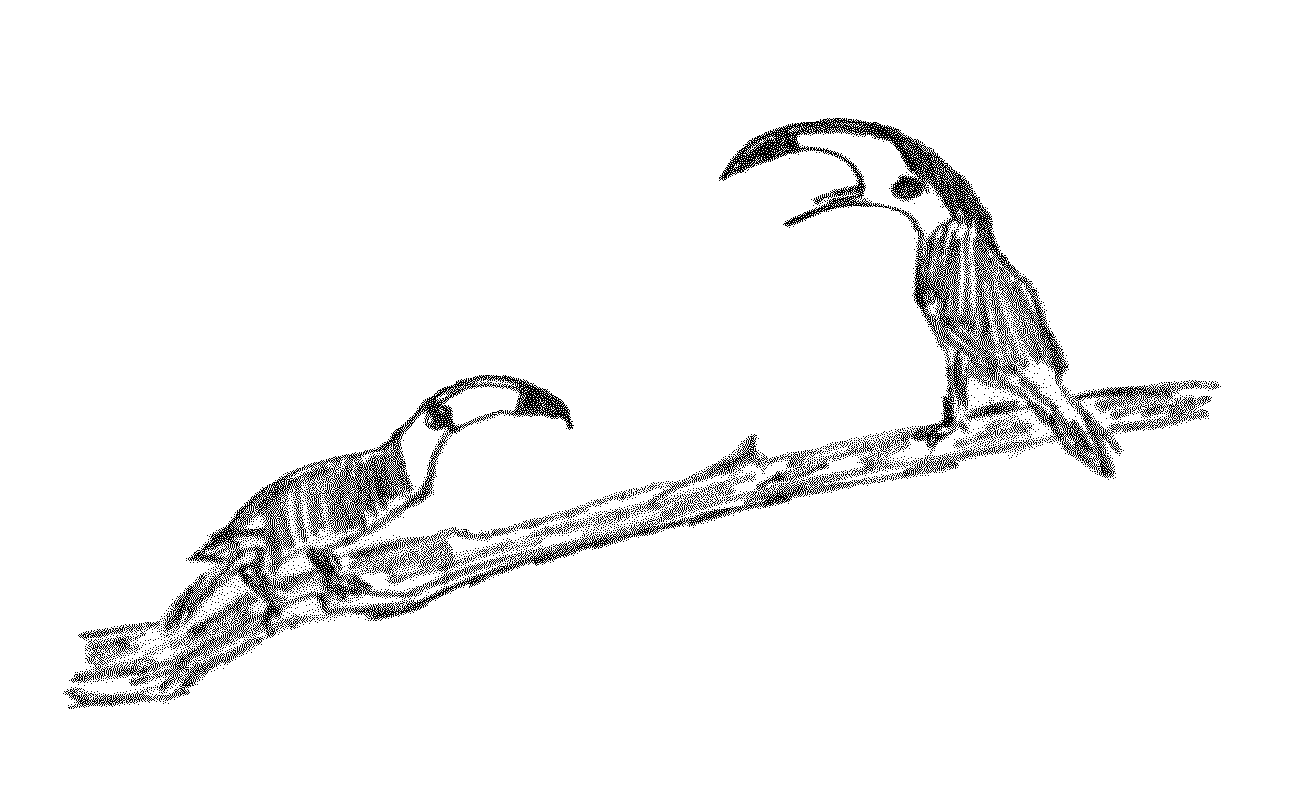
\includegraphics[width=166pt]{tucan.png}
\end{center}

\clearpage % or \cleardoublepage
\phantomsection % fixes the link anchor
\addcontentsline{toc}{chapter}{\indexname}
\printindex

\clearpage % or \cleardoublepage
\phantomsection % fixes the link anchor
\addcontentsline{toc}{chapter}{Colophon}

\chapter*{Colophon}

The cover shows Rexx programmers with the tree representation of an XML
document. The origin of the graphic is unknown, but it appears to have been
scanned from a 19th century wood-cut. The other drawings, except for the
computer on this page, which was by Austin Yin, were made by Fei Huang for
this project and scanned by the author. The confusing graphics are by the
author.

The manual, along with the library and most of the things I've written since
1988, was prepared using Craig Durland's Mutt Editor. It was marked up
using the \LaTeX\ book class, with the array and longtable
packages.\footnote{The editor's macro language isn't Rexx, and \LaTeX\ isn't
XML. So sue me.} The PDF version of the manual was formatted using PDF\TeX,
and the links were generated automatically by the hyperref package.

The body text is Times Roman with examples in Courier. These fonts were chosen
because they don't have to be embedded in PDF files, and I wanted to at least
nominally keep the size down.

Many people have contributed to this project, either directly or
indirectly. I hope that some of them find it helpful.

\vspace{3pt}

\vfil

\begin{center}
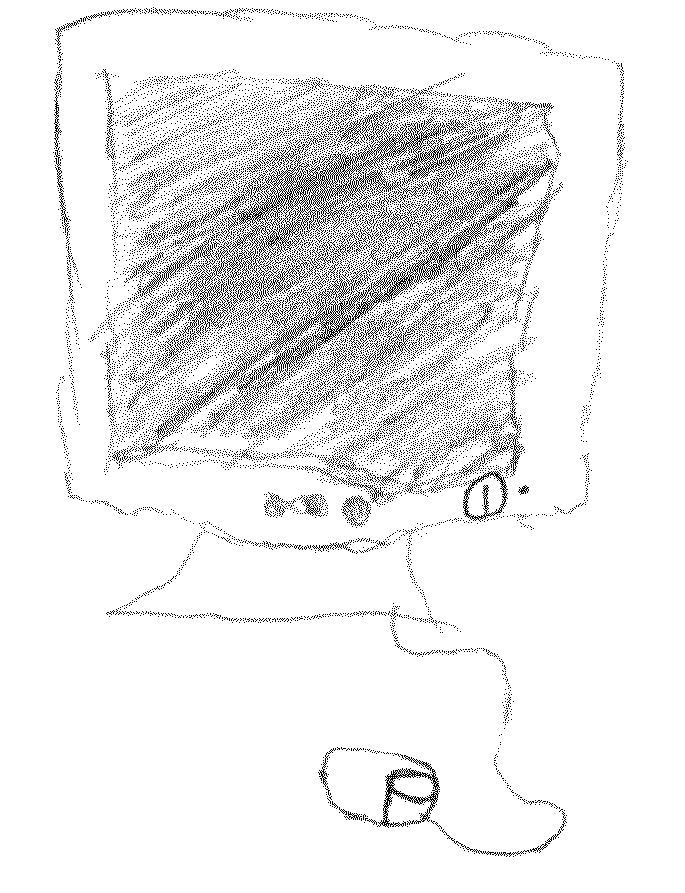
\includegraphics[width=88pt]{computer.png}
\end{center}


\end{document}

